% compile-latex options: --jobname sys
% compile-latex options: --jobname spoly

\documentclass{iutv2013}
\subtitle{Cours complet}
\author{G. Santini, J.-C. Dubacq}%

\let\Return\relax
\usepackage{keystroke}

% Pour le caractère du curseur
\usepackage{marvosym}
\newcommand{\cursor}{\Rectsteel}

% FORMATAGE LINUX IN-LINE
\newcommand{\lin}[1]{\texttt{#1}}
\newcommand{\linbox}[1]{\colorbox{solarizedRebase02}{\textbf{\texttt{#1}}}}

% Formatage d'un terminal et de ses commandes et affichages
\newcommand{\promptP}[4][\~{}]{%
  \fboxsep=0pt%
  \colorbox{solarizedRebase02}{%
    \parbox{#2}{%
      \lin{%
	{\color{solarizedRed} login}@{\color{solarizedGreen} host}\string:{\color{solarizedBlue}#1}\$ #3\ifx#4\relax\relax\else\\\emph{#4}\fi}}}}
\newcommand{\mpromptP}[2]{\centerline{\fcolorbox{black}{solarizedRebase02}{\parbox{#1}{#2}}}}
\newcommand{\prompt}[3][\~{}]{\promptP[#1]{85mm}{#2}{#3}}
\newcommand{\mprompt}[1]{\mpromptP{95mm}{#1}}
\newcommand{\promptS}[3][\~{}]{\promptP[#1]{54mm}{#2}{#3}}
\newcommand{\mpromptS}[1]{\mpromptP{55mm}{#1}}
\newcommand{\promptT}[3][\~{}]{\promptP[#1]{34mm}{#2}{#3}}
\newcommand{\mpromptT}[1]{\mpromptP{35mm}{#1}}
\newcommand{\promptM}[3][\~{}]{\promptP[#1]{64mm}{#2}{#3}}
\newcommand{\mpromptM}[1]{\mpromptP{65mm}{#1}}


% Man
\newcommand{\manpage}[2][\relax]{%
  \ifx#1\relax\mymanpage{#2}{#2}\else\mymanpage{#1}{#2}\fi
}
\newcommand{\mymanpage}[2]{%
  \begin{frame}%\frametitle{Manuel de #2}
    \def\mantitle{#2}
    \input{Commandes/#1.tex}%
  \end{frame}
}

% Formatage des la description des commandes

%SYNTAXE
\newcommand{\synt}[3]{\begin{alertblock}{Syntaxe pour \mantitle}
\begin{center}\lin{#1 \textit{#2} #3}\end{center}
\end{alertblock}}
\newcommand{\dsynt}[6]{\begin{alertblock}{Syntaxe pour \mantitle}
\begin{center}\parbox{\linewidth}{\lin{#1 \textit{#2} #3}\\
\lin{#4 \textit{#5} #6}}
\end{center}
\end{alertblock}}

%DESCRIPTION
\newcommand{\desc}[1]{\begin{block}{Description}#1\end{block}}

%EXEMPLE
\newcommand{\expl}[2][]{\begin{exampleblock}{Exemple d'utilisation: #1}\footnotesize{#2}\end{exampleblock}}

% Pour les arborescences
\usepackage{dirtree}
\renewcommand*\DTstyle{\small}
\renewcommand*\DTstylecomment{\small}
\DTsetlength{0.2em}{1em}{0.2em}{0.4pt}{1.6pt}
\newcommand{\DTd}[1]{{\color{solarizedBlue}#1/}}
\newcommand{\DTg}[1]{{\color{solarizedGreen}#1/}}
\newcommand{\DTfcomment}[1]{\DTcomment{~~\color{solarizedYellow}{#1}}}

\newcommand{\fileform}[3][6cm]{%
	\vspace{3pt}\small
	\begin{tabular}{|l|l}
		\cline{1-1}\textbf{#2}&\\
		\hline
		\multicolumn{2}{|l|}{
			\begin{minipage}{#1}
				\lin{\\#3\\}
			\end{minipage}
		}\\
		\hline
	\end{tabular}
	\vspace{3pt}
}


\begin{document}
\beamertitle
\begin{frame}{Organisation du module}
  \begin{alertblock}{Remerciements}
    \begin{itemize}
    \item Les cours et exercices de ce module sont directement inspirés
      des documents de \textbf{M. Bosc}, \textbf{J.-C. Dubacq} et \textbf{G. Santini}.
    \item D'autres intervenants ont participé à l'élaboration des supports.
    \end{itemize}
  \end{alertblock}
  \begin{block}{Les enseignements}
    \begin{itemize}
    \item 12 sessions de 4h et du travail personnel \dots
    \item 6 sessions pour la présentation générale du système
      d'exploitation Linux,
    \item 6 sessions pour la théorie de base du codage informatique 
    \end{itemize}
  \end{block}
  \begin{alertblock}{Votre présence est obligatoire}
    \begin{itemize}
    \item Contrôle des présences.
    \item Rapport des absences.
    \end{itemize}
  \end{alertblock}
  \begin{block}{L'évaluation}
    \begin{itemize}
    \item Une composition après la sixième session (sur papier ou sur
      ordinateur).
    \item Une composition à la fin du module (sur papier ou sur
      ordinateur).
    \end{itemize}
  \end{block}
\end{frame}

\section{Généralités}
\subsection{Qu'est-ce qu'un ordinateur?}
%%%%%%%%%%%%%% 
\begin{frame}{Définition}
  \begin{definition}[Ordinateur]\it
    Machine électronique programmable capable de réaliser des calculs
    logiques sur des nombres binaires.
  \end{definition}
  \begin{block}{C'est une machine\hfill\emph{Hardware}}
    Le fonctionnement d'un ordinateur est basé sur une architecture
    matérielle (processeur, support de stockage, interfaces
    utilisateurs, connexion, \dots) dont le fonctionnement est soumis
    aux lois de la physique.
  \end{block}
  \begin{block}{C'est une machine programmable\hfill\emph{Software}}
    Cette machine est capable de remplir des tâches différentes selon
    les instructions qui lui sont adressées. Ces instructions, rédigées
    sous forme de programmes par les informaticiens, sont traitées en
    fin de course par le matériel de l'ordinateur.
  \end{block}
  \begin{alertblock}{Interaction Hardware/Software}
    La plupart du temps, l'informaticien n'a pas a interagir directement
    avec le matériel. Pour traiter avec les composants, tous les
    ordinateurs disposent d'une couche logicielle appelée
    \emph{système d'exploitation}. Cette couche est en charge de faire la
    passerelle entre l'informaticien, ses outils, les programmes qu'il
    développe et, les composants et leur fonctionnement.
  \end{alertblock}
\end{frame}

\subsection[Composants et principes]{Les composants principaux et les
  principes de fonctionnement d'un ordinateur}
\begin{frame}{Les interfaces}
  \begin{columns}
    \begin{column}[T]{6cm}
      \begin{block}{La forme classique}
        \begin{itemize}
        \item Un ordinateur est classiquement composé d'une unité
          centrale et de périphériques matériels (écran, clavier,
          souris, disques durs, imprimantes/scaner, \dots).
        \item Les interfaces permettent l'interaction avec
          l'environnement (utilisateurs ou autres).
        \end{itemize}
      \end{block}
    \end{column}
    \begin{column}[T]{5cm}
      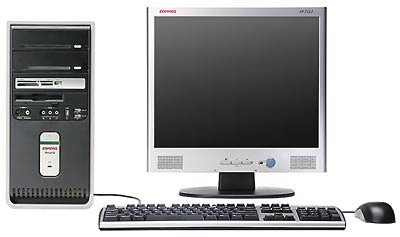
\includegraphics[width = 5cm]{img/s01/uc_ecran_clavier.png}
    \end{column}
  \end{columns}
  \vspace{1cm}
  \begin{columns}
    \begin{column}[T]{6cm}
      \begin{block}{Des formes très variées}
        \begin{itemize}
        \item Les ordinateurs modernes sont multiformes,
        \item Ils remplissent des tâches très variées.
        \end{itemize}
      \end{block}
    \end{column}
    \begin{column}[T]{5cm}
      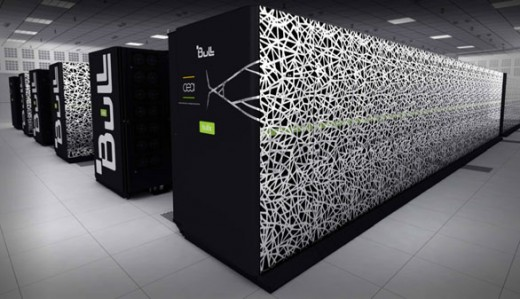
\includegraphics[width = 2.5cm]{img/s01/cluster_cea.png}\hspace{1cm}
      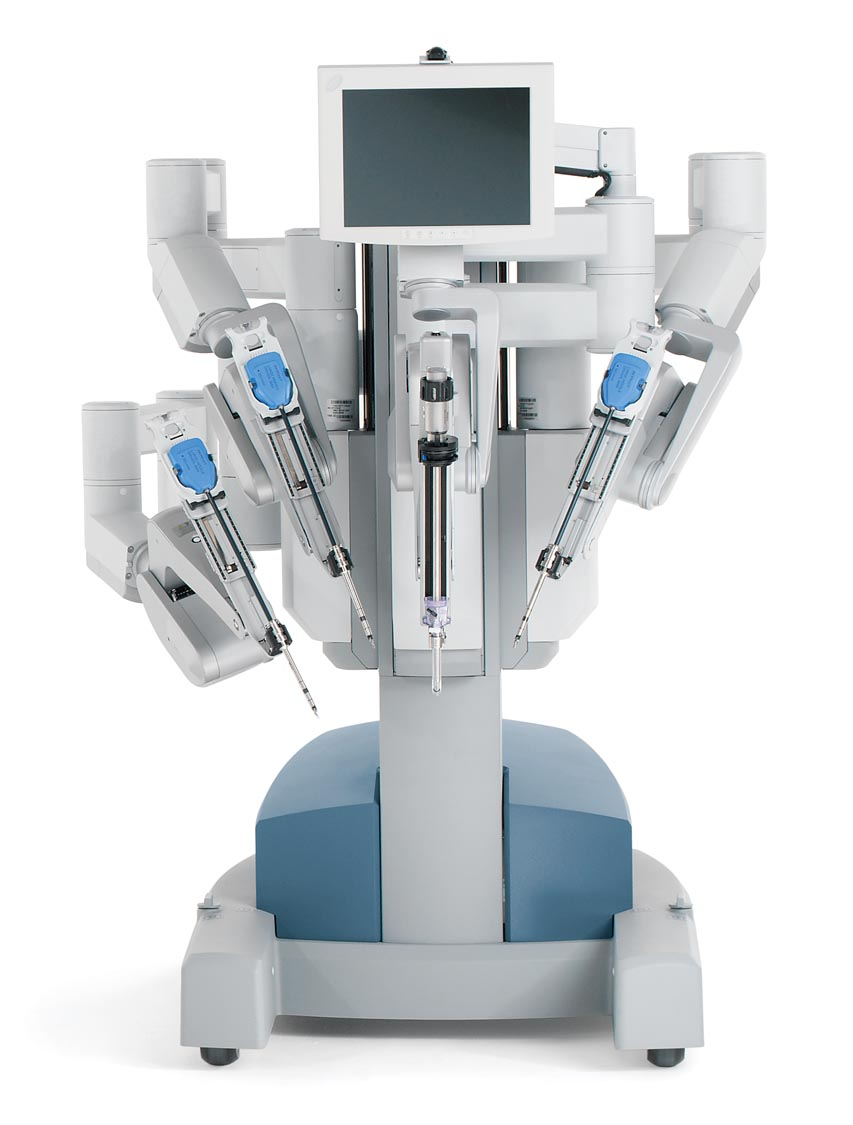
\includegraphics[height = 1.5cm]{img/s01/Davinci-Robot-chirurgical-001.jpg}\\
      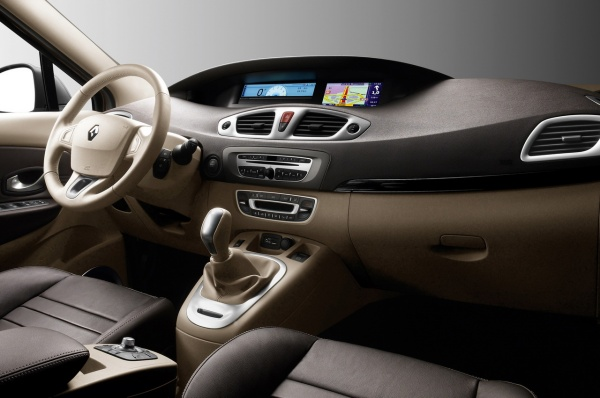
\includegraphics[width =
      2.5cm]{img/s01/scenic_console_centrale.png}\hspace{1cm}
      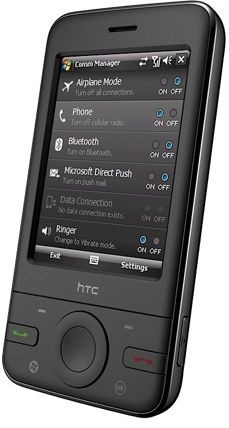
\includegraphics[height = 1.5cm]{img/s01/telephone_tc_linux.png}
    \end{column}
  \end{columns}
\end{frame}

\begin{frame}{Points communs et différences}
  \begin{block}{Matériel commun}
    \begin{itemize}
    \item Des capacités de calcul: CPU et/ou GPU
    \item De la mémoire : RAM, Disque dur, \dots
    \end{itemize}
  \end{block}
  \begin{block}{Logiciels similaires}
    \begin{itemize}
    \item Pour dialoguer avec le matériel : Système d'exploitation, Firmware
    \item Pour accomplir ses tâches : logiciels, programmes, \dots
    \end{itemize}
  \end{block}
  \begin{alertblock}{Périphériques différents}
    \begin{itemize}
    \item Interfaces : Connexions réseau, écrans, claviers, \dots
    \end{itemize}
  \end{alertblock}
\end{frame}

\begin{frame}{La mémoire : une bibliothèque plus ou moins grande}
  \begin{block}{Le guichet et les fiches numérotées}
    \begin{itemize}
    \item Permet de stocker des informations comme nombre entiers
    \item[\dialoginformation] Toute information \emph{d'un ordinateur} peut être vue comme des nombres entiers
    \item Fiches numérotées par des adresses entières. Exemple: la fiche numéro 221 contient la valeur 18.
    \item[\dialogwarning] L'interprétation de l'information n'est pas incluse → notion de codage
    \end{itemize}
  \end{block}
  \begin{block}{Les performances}
    \begin{itemize}
    \item Guichet unique d'accès : une requête à la fois.
    \item On peut \emph{écrire} une valeur dans une fiche ou \emph{lire} une fiche, rien d'autre
    \item[\dialogsystem] On peut aussi demander un paquet de fiches contiguës → plus rapide!
    \item Notion de \emph{mémoire cache hiérarchique} : copie de Grande Bibliothèque dans une bibliothèque plus rapide et plus petite
    \item Performance : de l'ordre de 20 Go/s
    \end{itemize}
  \end{block}
\end{frame}

\begin{frame}{Le processeur : un moteur à quatre temps}
  \begin{block}{Un assemblage hétéroclite}
    \begin{itemize}
    \item Une unité de calcul qui sait faire... des calculs (simples)
    \item Des registres qui retiennent chacun \textnormal{une} valeur
    \item Des circuits de transmission contrôlables électriquement, qui
      relient les composants entre eux et aussi le processeur à la
      mémoire.
    \item Une unité de contrôle qui découpe une \emph{instruction} en
      morceaux et contrôle les transmissions des circuits en fonction
      des résultats.
    \end{itemize}
  \end{block}
  \begin{block}{Un cycle vital immuable}
    Le processeur effectue des opérations très rapidement, en suivant toujours la même procédure générale :
    \begin{enumerate}
    \item \emph{Récupération} de l'instruction : on demande à la mémoire
      le contenu d'une adresse, dont la valeur est trouvée dans le
      registre PC.
    \item \emph{Décodage} de l'instruction : la valeur est analysée, les
      circuits de transmission sont mis en route
    \item \emph{Exécution} de l'instruction : l'unité de calcul est
      mobilisée
    \item \emph{Écriture des résultats} : un registre sauvegarde le
      résultat, le PC est augmenté de 1
    \end{enumerate}
    Des instructions spécifiques, au lieu de calculs, permettent d'accéder
    à la mémoire en lecture (étape 2) ou écriture (étape 4) au lieu des
    registres.
  \end{block}
\end{frame}
\begin{frame}
  \begin{block}{L'étonnante efficacité}
    \begin{itemize}
    \item[\dialogwarning] Les instructions données doivent être simples (opérations arithémtiques entre deux valeurs, tests élémentaires uniquement).
    \item Les registres sont très rapides ; la durée d'un cycle est de l'ordre de la nanoseconde.
    \item Toute opération complexe est divisée par un humain en opérations élémentaires → \emph{programmation}.
    \item Les instructions forment un code compact appelé \emph{code machine}.
    \item[\dialogsystem] Analogie : pour faire une multiplication, on
      peut faire plein d'additions et tester si on arrive à 0.
    \end{itemize}
  \end{block}
  \begin{block}{Les grands défauts}
    \begin{itemize}
    \item[\dialogerror] Aucune intelligence
    \item[\dialogerror] Aucune compréhension réelle des valeurs manipulées
    \item[\dialogerror] On ne peut pas tout surveiller → \emph{bugs}
    \end{itemize}
  \end{block}
\end{frame}

\begin{frame}{L'horizon matériel}
  \begin{block}{Interaction avec le matériel}
    \begin{itemize}
    \item Heureusement le programmeur ou l'utilisateur n'interagit pas
      directement avec le matériel (sauf pour remplacer une pièce
      défectueuse ou connecter un nouveau matériel \dots). Le dialogue
      avec l'architecture matériel est l'affaire de programmes dédiés.
    \item Plusieurs couches logicielles existent entre le matériel et
      l'utilisateur: les \textit{firmwares}, le noyau du système et les
      outils et programmes du système d'exploitation.
    \item La plupart des logiciels que vous serez amené à développer
      n'interagiront qu'indirectement avec le matériel par le filtre des
      librairies système.
    \end{itemize}
  \end{block}
  \begin{alertblock}{Haut Niveau $\rightarrow$}
    \begin{itemize}
    \item Logiciel,langages de programmation, \dots
    \item[\dialoginformation] C'est le domaine de l'informatique et des
      informaticiens
    \item[\dialogsystem] Une interface: Le système d'exploitation
    \end{itemize}
  \end{alertblock}
  \begin{alertblock}{Bas niveau}
    \begin{itemize}
    \item \textit{Firmwares}, exécution des instructions machine, \dots
    \item C'est le domaine de la physique et des électroniciens.
    \end{itemize}
  \end{alertblock}
\end{frame}

% XXXX Insérer schéma fonctionnement hardware <=> kernel <=> OS <=> apps

\section{Le système d'exploitation}
\subsection{La fonction du système d'exploitation}
\begin{frame}{Le système d'exploitation}
  Le système d'exploitation permet de développer des programmes sans
  tenir compte de la complexité physique de la machine. Les programmes
  utilisent des fonctionnalités standardisées d'accès aux ressources
  matérielles.
  \begin{columns}
    \begin{column}{5.5cm}
      \begin{block}{Côté Système, l'O.S.}
        \begin{itemize}
        \item coordonne l'utilisation des ressources (par exemple quel «
          programme » utilise le processeur à un moment donné,
          allocation de la mémoire, \dots),
        \item assure la maintenance et la fiabilité du système (par exemple
          gestion des fichiers, de la sécurité informatique, \dots)
        \item fournit des services commun à tous les programmes
        \end{itemize}
      \end{block}
      \begin{block}{Côté utilisateur, l'O.S.}
        \begin{itemize}
        \item facilite l'accès et l'utilisation des ressources
          matérielles,
        \item propose une interface de programmation permettant
          d'utiliser ces matériels
        \end{itemize}
      \end{block}
    \end{column}
    \begin{column}{6cm}
      \begin{center}
        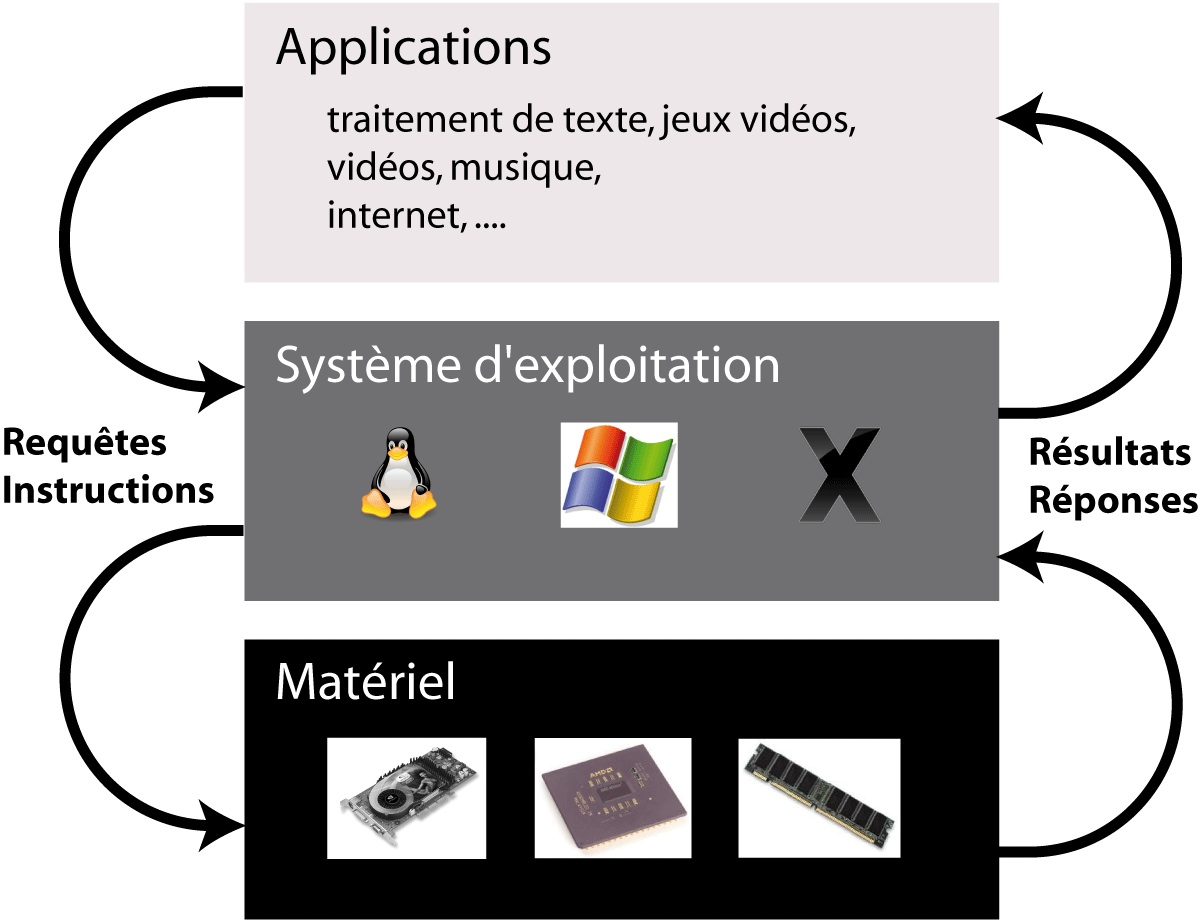
\includegraphics[width=6cm]{img/s01/OS_interface_2.jpg}
      \end{center}
    \end{column}
  \end{columns}
\end{frame}

\subsection{La multiplicité des systèmes existants}
\begin{frame}{Les différents systèmes d'exploitation}
  \begin{columns}
    \begin{column}{5.5cm}
      \begin{block}{Beaucoup d'OS différents existent:}
        Chaque architecture matérielle demande un système d'exploitation
        adapté. Certain systèmes d'exploitation sont plus souples et
        prennent en charge des architectures matérielles multiples.
      \end{block}
      \begin{center}
        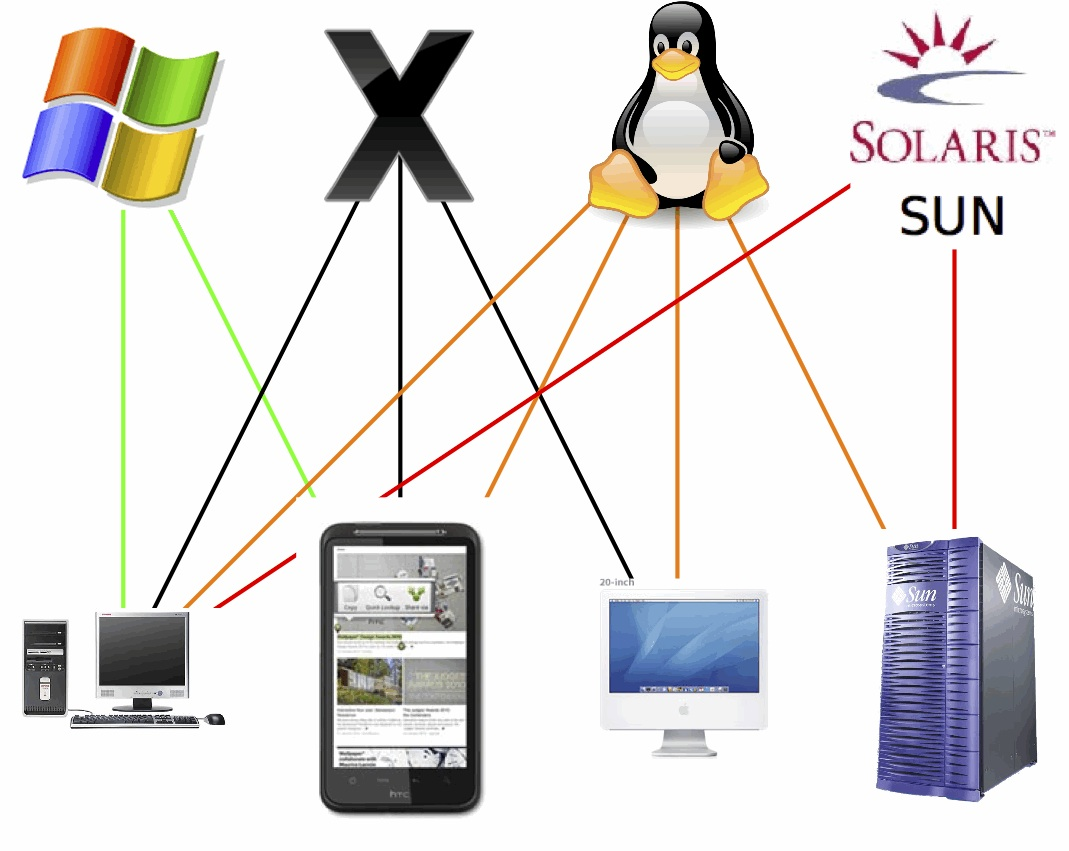
\includegraphics[width=5.5cm]{img/s01/OS_archi.jpg}
      \end{center}
    \end{column}
    \begin{column}{5.5cm}
      \begin{block}{Trois OS se distinguent:}
        Windows est le système d'exploitation le plus utilisé, OS X est réputé le plus simple et Linux est le système d'exploitation le plus souple.\\
        Statistiques au 5 janvier 2011: \url{http://gs.statcounter.com/}\\
        \begin{itemize}
        \item 90\% des ordinateurs utilisent Windows,
        \item il existe plus de 600 distributions Linux\dots
        \end{itemize}
      \end{block}
      \vrule
      \begin{center}
        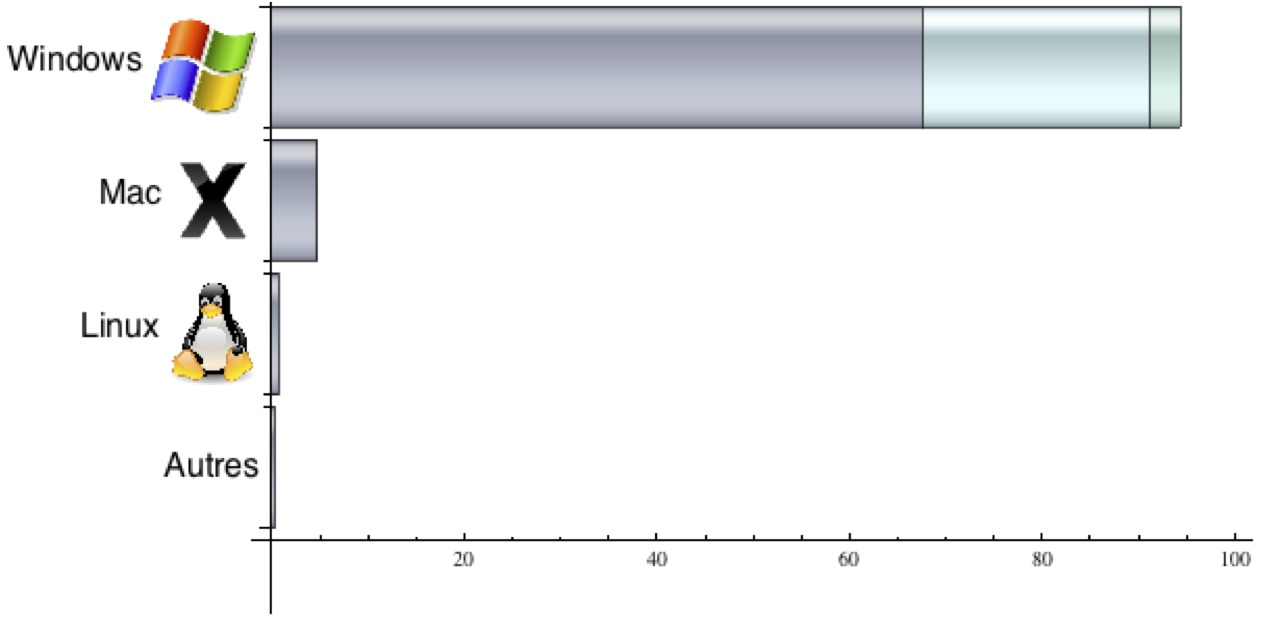
\includegraphics[width=5.5cm]{img/s01/OS_utilises.jpg}
      \end{center}
    \end{column}
  \end{columns}
\end{frame}

\subsection{Comparatif}
\begin{frame}{Les différents systèmes d'exploitation}
  \begin{columns}
    \begin{column}{58mm}
      \begin{block}{\center 
\includegraphics[height=1cm]{img/s01/Tux.png}\\Linux}
        \begin{itemize}
        \item Non propriétaire: Gratuit le plus souvent
        \item Ouvert: sources disponibles
        \item Flexible: sources modifiables
        \item Puissant: Programmable
        \item Communauté active: entraide des utilisateurs
        \item Plus complexe: plutôt pour les informaticiens (interfaces
          de programmation optimisées)
        \end{itemize}
      \end{block}
    \end{column}
    \begin{column}{58mm}
      \begin{block}{\center 
\includegraphics[height=1cm]{img/s01/Windows_logo.png}\\Windows}
        \begin{itemize}
        \item Propriétaire: Payant
        \item Sources non disponibles
        \item Sources non modifiables
          % \item Plus difficilement programmable
        \item Communauté active: nombreux utilisateurs, services payants
        \item Plus ergonomique: pour les utilisateurs (interfaces
          d'utilisation optimisées)
        \end{itemize}
        \vrule
      \end{block}
    \end{column}
  \end{columns}
  \begin{alertblock}{Les systèmes, en constante évolution}
    Depuis une dizaine d'année, Linux et Windows ont beaucoup évolué. La
    plupart des distributions Linux proposent des systèmes
    d'installation automatisés, des outils de bureautique ressemblant
    aux suites commerciales. Il bénéficie en outre d'une sécurité accrue
    à l'heure des virus et autres failles de sécurité. Windows propose
    de plus en plus de fonctionnalités empruntées à Linux.
  \end{alertblock}
\end{frame}

\section{Le système Linux}
\subsection{Un peu d'histoire}
\begin{frame}{Un peu d'histoire}
  \begin{block}{GNU-Linux}
    \begin{itemize}
    \item Le système GNU-Linux est la rencontre d'une technologie, le
      noyau Linux et d'une philosophie de développement et de
      diffusion. C'est un système au développement collaboratif (par une
      communauté) qui est distribué librement et permet l'utilisation de
      tous les logiciels libres développés pour son architecture.
    \item Le noyau Linux est historiquement une version libre du système
      UNIX développé initialement par le Finlandais Linus Torvalds à
      partir du début des années 1990.
    \item Le projet GNU est celui du développement collaboratif et libre
      d'un système d'exploitation libre initié par Richard Stallman en
      1983.
    \end{itemize}
  \end{block}
  \begin{block}{Aujourd'hui}
    \begin{itemize}
    \item C'est un système très largement diffusé et utilisé sur lequel
      ont été développées plusieurs distributions (qui sont des suites
      logicielles qui accompagnent le noyau).
    \item Initialement confidentiel et réservé à des spécialistes avec
      des interfaces rudimentaires, il est aujourd'hui toujours plus
      ergonomique et automatisé pour les non spécialistes, mais laisse
      les outils et interfaces de bas niveau disponibles au plus grand
      nombre.
    \item On notera par exemple l'existence de nombreuses interfaces
      graphiques \textit{Bureaux} (GNOME, KDE, \dots) de nombreux
      paquetages pré-compilées, de nombreux outils d'administration et
      de services (protocoles, \dots)
    \end{itemize}
  \end{block}
  
\end{frame}
\subsection{Debian: La distribution utilisée à l'IUT}
\begin{frame}{À l'IUT: Debian}
  \begin{block}{Une distribution téléchargeable}
    \begin{columns}
      \begin{column}{8cm}
        \url{http://www.debian.org/}\\
      \end{column}
      \begin{column}{3cm}
        
\includegraphics[width=1cm]{img/s01/openlogo-100.png}
      \end{column}
    \end{columns}
  \end{block}
  \begin{block}{Pour ce cours}
    \begin{itemize}
    \item Les concepts abordés dans ce module sont généraux.
    \item Il pourront être testés sur tous les systèmes Linux (avec de très faibles variantes).
    \item Il vous est possible d'installer une version de Linux sur votre ordinateur personnel (installation ou version Live) pour votre pratique personnelle et la préparation de l'examen.
    \item Une pratique régulière devrait vous assurer une bonne note à peu de frais\dots
    \end{itemize}
  \end{block}
  \begin{alertblock}{Pour vous préparer à l'examen}
    Il vous est possible:
    \begin{itemize}
    \item d'utiliser Linux dans les salles machines,
    \item d'installer une version de Linux sur votre ordinateur personnel (installation ou version Live).
    \end{itemize}
  \end{alertblock}
\end{frame}

\subsection{Un système multi-utilisateurs}
\begin{frame}{Un système avec plusieurs utilisateurs}
  \begin{block}{Des utilisateurs et des droits}
    \begin{itemize}
    \item Chaque personne accédant au système est identifiée par un
      \textbf{nom d'utilisateur} (dit \textit{login}) et un mot de passe
      (dit \textit{password}).
    \item Chaque utilisateur bénéficie de permissions: exécution de
      certains programmes, lecture de certaines données, écriture de
      fichiers seulement dans certains répertoires.
    \item Chaque utilisateur bénéficie d'un \emph{espace de travail}
      réservé sur le disque. C'est un répertoire de l'arborescence dans
      lequel l'utilisateur a tous les droits: il peut y créer des
      sous-répertoires, y écrire des fichiers, y installer des
      programmes et applications. Toutes ses données et préférences
      personnelles y sont regroupées.
    \item Ce répertoire est appelé "Répertoire Personnel" ou
      \textit{"Home Directory"}. Il est en général placé dans un
      répertoire qui s'appelle \lin{/home/} et porte le nom de
      l'utilisateur.
    \end{itemize}
  \end{block}
  \begin{alertblock}{Superutilisateur - Root}
    \begin{itemize}
    \item certains utilisateurs ont des permissions étendues pour
      administrer le système et effectuer des opérations interdites à
      l'utilisateur normal.
    \item l'utilisateur \lin{root} a tous les droits dans le système
      (par exemple il peut changer les permissions de n'importe quel
      fichier, il fixe les noms d'utilisateur et les mots de passe, il
      peut installer des programmes et librairies dans les répertoires
      système, \dots)
    \end{itemize}
  \end{alertblock}
\end{frame}

\begin{frame}{Identification en 2 étapes}
  \begin{center}
    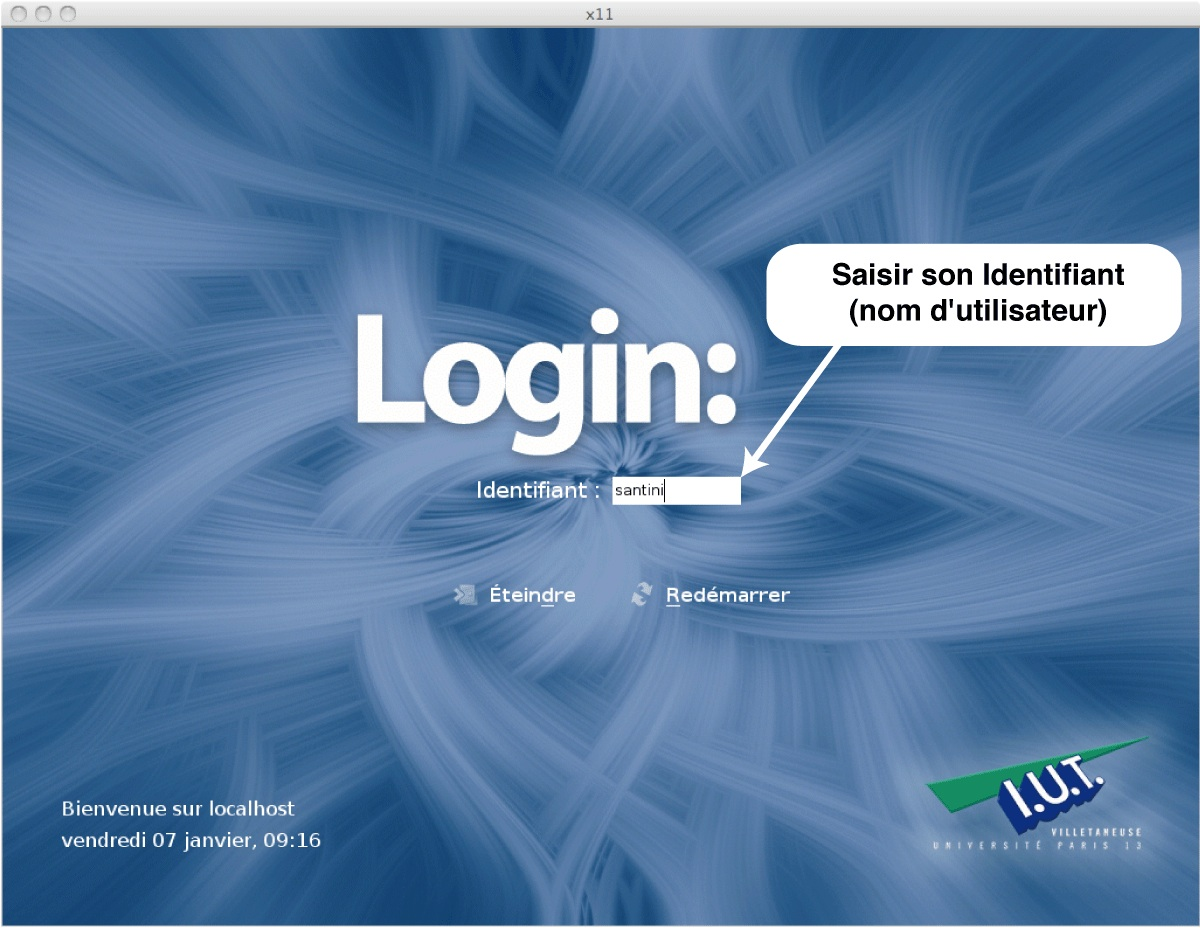
\includegraphics[width=8cm]{img/s01/linux_login.jpg}
  \end{center}
  \begin{block}{Étape \#1}
    S'identifier en donnant au système son nom d'utilisateur
  \end{block}
\end{frame}
\begin{frame}{Identification en 2 étapes}
  \begin{center}
    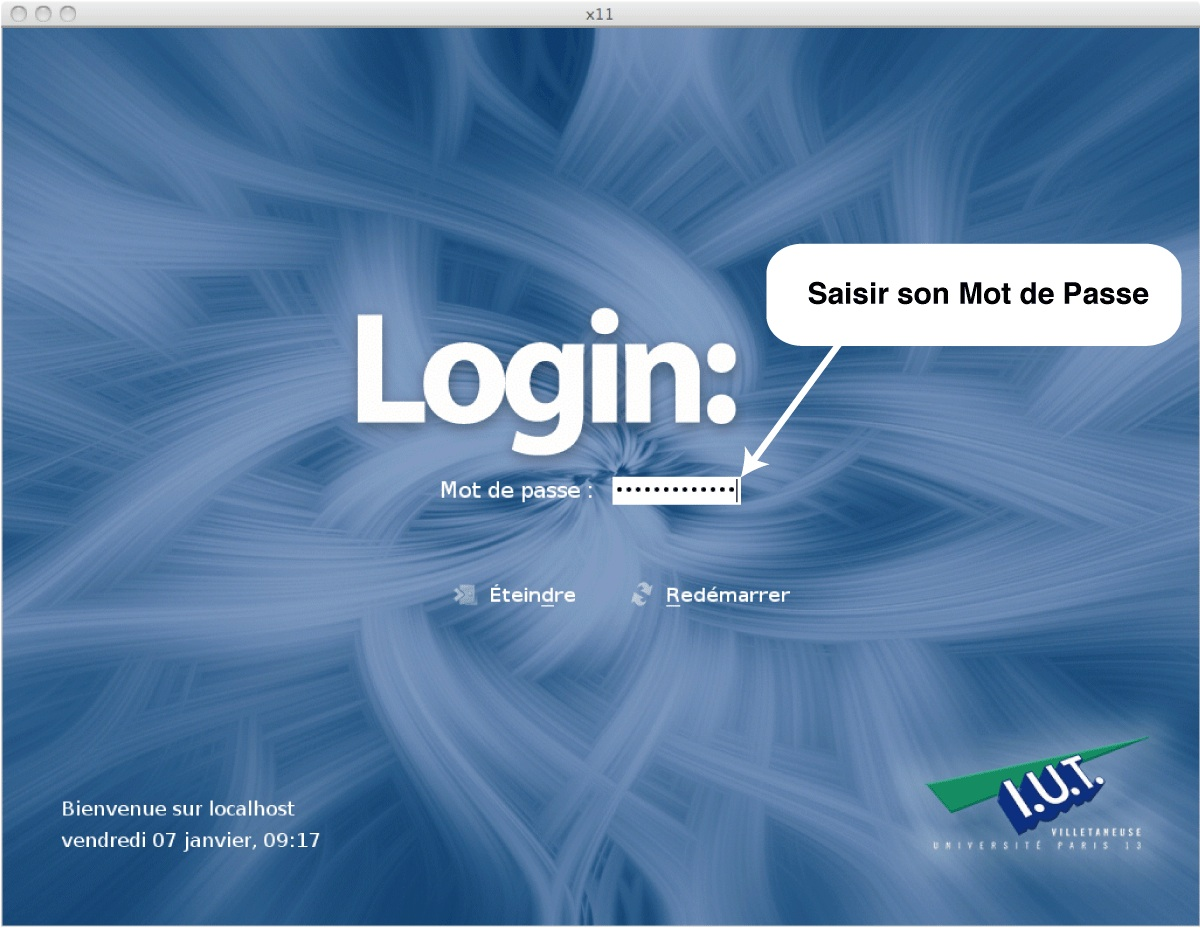
\includegraphics[width=8cm]{img/s01/linux_passwd.jpg}
  \end{center}
  \begin{block}{Étape \#2}
    Valider son identité avec le mot de passe
  \end{block}
\end{frame}
\begin{exercice}
  Ce TP est un premier contact avec le système d'exploitation Linux. Il
  vous permettra d'appréhender les différences entre cet OS et ceux que
  vous pouvez avoir l'habitude d'utiliser (Windows, MacOS-X). Nous
  présenterons au cours du TP les grandes lignes de l'environnement de
  travail GNOME, la façon dont on peut interagir avec le système
  d'exploitation au moyen de l'outil "Terminal" ainsi que les outils de
  base pour envoyer des mails (configuration de votre compte mail à
  l'IUT) et pour obtenir de l'information sur internet (notamment sur
  Linux). Il existe de nombreuses versions gratuites ou payantes de
  Linux. La distribution installée à l'IUT se nomme Debian et est
  téléchargeable depuis \url{http://www.debian.org/}.
  \begin{exercicelet}{Connexion initiale}
    \begin{questions}
    \item Lorsqu'on allume l'ordinateur un laps de temps est nécessaire
      pour charger le système d'exploitation. Au terme de ce chargement,
      une interface graphique propose à l'utilisateur de s'identifier.
      Linux est un système d'exploitation multi-utilisateur. Chaque
      utilisateur doit systématiquement s'identifier ("login") auprès du
      système pour avoir le droit de l'utiliser. Une fois identifié,
      l'utilisateur à accès a ses fichiers et son espace de travail
      personnel. Une fois qu'il a fini d'utliser le système,
      l'utilisateur se déconnecte ("logout"). La période entre
      l'identification et la connexion est appellée "session
      d'utilisation". Démarrez votre ordinateur.
    \item Connectez-vous! Votre identifiant est votre numéro d'étudiant,
      votre mot de passe est votre numéro INE.  Attention: les
      identifiants et les mots de passe sont sensibles à la casse. Cela
      veut dire que les caractères majuscules et minuscules sont
      distingués.
    \end{questions}
  \end{exercicelet}
\end{exercice}


\subsection{Une interface graphique}
\begin{frame}{Accès au système}
  \begin{center}
    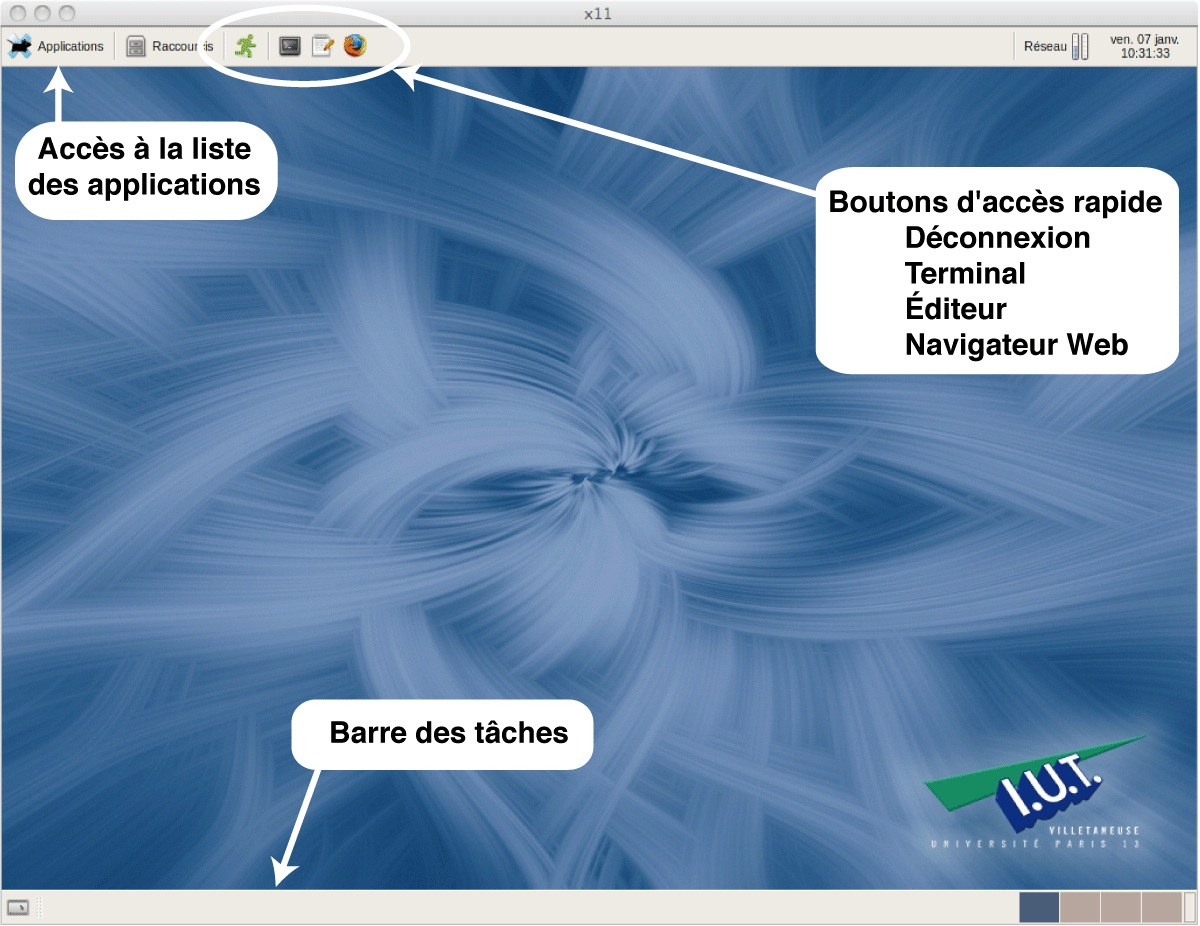
\includegraphics[width=8cm]{img/s01/Gnome_desktop.jpg}
  \end{center}
  \begin{block}{Le bureau GNOME}
    Parmi les différents environnements graphiques existants, vous
    utiliserez l'environnement GNOME (\url{http://www.gnomefr.org/}).
  \end{block}
\end{frame}
\begin{exercice}
  \begin{exercicelet}{Métaphore du bureau}
    Contrairement aux systèmes d'exploitation propriétaires,
    l'environnement de travail (bureau) n'est pas directement lié au
    système d'exploitation. Les deux environnements de travail les plus
    utilisés sous Linux sont GNOME (\url{http://www.gnomefr.org/}) et
    KDE (\url{http://fr.kde.org/})
    
    L'environnement choisi à l'IUT est GNOME .  Une fois la session
    lancée et l'environnement chargé, vous arrivez dans un espace de
    travail appelé \emph{bureau}.  Cet environnement de travail est
    assez proche de celui qui peut être proposé par les systèmes
    d'exploitation propriétaires. Au moyen de la souris, vous pouvez
    intéragir avec le système. En cliquant sur les éléments graphiques,
    vous pouvez ouvrir des menus, lancer des programmes, quitter le
    système...
    \begin{questions}
    \item Identifier la barre de menu, la barre de tâches et le bureau.
    \item Dans cet environnement, identifiez deux façons de lancer le
      navigateur internet
      (Firefox 
\includegraphics[height=2ex]{img/s01/firefox.png}), et
      l'application terminal
      (
\includegraphics[height=2ex]{img/s01/terminal.png}).
    \end{questions}
  \end{exercicelet}
\end{exercice}
\begin{exercice}
  \begin{exercicelet}{Lancement d'applications}
    Comme la plupart des systèmes d'exploitation modernes, la
    distribution de Linux mise à votre disposition est un système
    multi-tâches. Cela signifie, que vous pouvez exécuter en parallèle
    plusieurs applications. Il n'est pas rare que lors d'une session
    vous lanciez plusieurs programmes où chaque programme est associé à
    une fenêtre. À la suite des exercices précédents, vous devez avoir
    au moins 4 fenêtres ouvertes (même si elles ne sont pas toutes
    visibles à l'écran). Les fenêtres ouvertes apparaissent dans la
    barre des tâches située dans la partie basse de l'écran qui doit
    alors ressembler à ça:

    \centerline{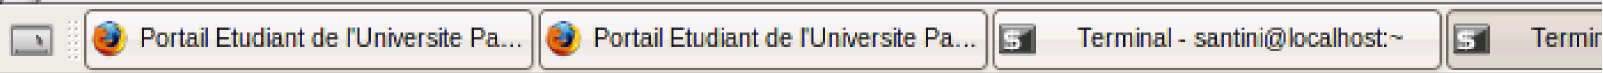
\includegraphics[width=.8\linewidth]{img/s01/barredestaches.png}}

    \begin{questions}
    \item Donnez différentes façons de passer d'un programme à l'autre,
      d'une fenêtre à l'autre, (au moyen de la souris ou du clavier)?
      Qu'observez-vous au niveau de la barre des tâches lorsque vous
      passez d'une application à l'autre?
    \item Identifiez l'outil permettant de passer d'un bureau à l'autre.
      Décrivez dans quelles situations ces bureaux peuvent-être utiles.
      Trouvez comment on déplace une fenêtre depuis un bureau vers un
      autre.
    \item Placez sur les bureaux 1 et 2, une fenêtre de terminal chacun
      et sur les 3 et 4, une fenêtre de navigateur.
      \centerline{Résultat
        attendu: 
\includegraphics[height=2ex]{img/s01/barrepeuplee.png}}
    \item Expliquez la fonction de chacun des boutons placés dans le
      coin supérieur droit des fenêtres.  Fermez les fenêtres des
      programmes suivants: un terminal (bureau 1) et un navigateur
      (bureau 3).
    \end{questions}
  \end{exercicelet}
\end{exercice}

\subsection{Les logiciels disponibles}
\begin{frame}{Les logiciels disponibles}
  \begin{block}{Les suites bureautiques}
    \begin{itemize}
    \item Les suites bureautiques proposent les fonctionnalités grand
      public de traitement de texte, de tableur, de présentation, de
      dessin.
    \item Plusieurs suites gratuites existent en libre accès sous linux
      \begin{itemize}
      \item CalligraSuite (\url{http://www.calligra-suite.org/})
      \item OpenOffice (\url{http://fr.openoffice.org/})
      \item \dots
      \end{itemize}
    \end{itemize}
  \end{block}
  \begin{block}{Les programes dédiés}
    \begin{itemize}
    \item Navigateur Web, Client de messagerie, comme sous d'autres OS,
      de nombreuses solutions existent.
      \begin{itemize}
      \item Firefox, Opera, Konqueror, \dots
      \item Thunderbird, KMail, \dots
      \end{itemize}
    \item Des logiciels parmi les plus puissants:
      \begin{itemize}
      \item Manipulation et création d'images: GIMP, ImageMagick, \dots
      \item Modélisation 3D: Blender, \dots
      \end{itemize}
    \end{itemize}
  \end{block}
  \begin{block}{De nombreuses micro-application ou programmes}
    \begin{itemize}
    \item De nombreux programmes de conversion de format, de
      communication et de téléchargement existent en ligne de commande
      \dots
    \end{itemize}
  \end{block}
\end{frame}
\begin{exercice}
  \begin{exercicelet}{Éditeur de texte}
    Nous allons créer un nouveau fichier. Pour cela nous allons utiliser
    un outil fondamental pour tout programmeur: un éditeur de
    texte. Plusieurs éditeurs de texte sont à votre disposition (vous
    pouvez explorer le menu Applications \textrightarrow Accessoires ou
    Applications \textrightarrow Développement dans la barre de menu de
    GNOME).  À la différence de logiciels tels que Word, un éditeur de
    texte ne permet que de saisir du texte brut, sans mise en forme. Les
    programmes sont en général écrits dans un éditeur de texte.  Pour
    lancer un éditeur de texte trois moyens sont à votre disposition:
    \begin{itemize}
    \item Lancer l'application depuis le menu application,
    \item Lancer l'application depuis une icône du bureau,
    \item Lancer l'application depuis la ligne de comande, par exemple
      en tapant : \mprompt{ \prompt{gedit\Return}{}}
    \end{itemize}
    Ceci aura pour effet d'ouvrir une fenêtre de l'éditeur.
  \end{exercicelet}
\end{exercice}
\begin{exercice}
  \begin{exercicelet}{Éditeur de texte (suite)}
    \begin{questions}
    \item Tapez du texte dans la fenêtre et enregistrez le fichier dans
      votre répertoire personnel, avec le nom \verb|fichier_test_1.txt|.
    \item Définissez ce qu'est un \emph{raccourci clavier} et à quoi il
      sert (aidez-vous d'Internet si nécessaire).  Donnez une liste d'au
      moins 8 \emph{raccourcis clavier} standards les plus utilisés des
      éditeurs de texte.
    \item Modifiez le fichier texte \verb|fichier_test_1.txt| pour que
      le texte suivant y figure:
      \begin{quote}
        Ondoyons un poupon, dit Orgon, fils d'Ubu. Choux, bijoux, poux,
        puis du mou, du conflit, buvons non point un grog : un punch. Il
        but du vin itou, du rhum, du whisky, du coco, puis il dormit sur
        un roc.
      \end{quote}
    \item En utilisant les raccourcis clavier ou les menus et après les
      avoir testés, donnez les combinaisons ou procédures permettant de:
      \begin{itemize}
      \item Rechercher dans ce texte toutes les occurrences de la chaîne
        de caractères \texttt{oux}.
      \item Remplacer toutes les occurrences de la chaîne de caractères
        \texttt{oux}, par la chaîne de caractères \texttt{ou}.
      \item Supprimer toutes les occurrences de la chaîne de caractères
        \texttt{du}.
      \end{itemize}
    \item Enregistrez les modifications dans un nouveau fichier appelé
      \verb|fichier_test_2.txt|.
    \end{questions}
  \end{exercicelet}
\end{exercice}

\subsection{Distribution et accès aux logiciels}
\begin{frame}{Distribution et accès aux logiciels}
  \begin{columns}
    \begin{column}{6cm}
      \begin{block}{Licences libres (open source)}
        Elles permettent de :
        \begin{itemize}
        \item d'utiliser le logiciel,
        \item d'étudier et de modifier les sources,
        \item de redistribuer les sources, modifiées ou non.
        \end{itemize}
      \end{block}
    \end{column}
    \begin{column}{5cm}
      \begin{block}{Licences Propriétaires}
        Elles restreignent un ou plusieurs des droits listés \it{supra}.
      \end{block}
      \begin{block}{Gratuit ne signifie pas libre}
        Certains logiciels gratuits sont des logiciels propriétaires).
      \end{block}
    \end{column}
  \end{columns}
  \begin{block}{Copyright\copyright{} contre Copyleft\textcopyleft}
    Le Copyleft\textcopyleft utilise le cadre légal du copyright pour
    inverser les rapports de force: le code distribué peut être modifié
    et redistribué, mais uniquement avec les mêmes droits
    \textrightarrow Les logiciels qui dérivent des sources Copyleft ne
    peuvent être distribués hors Copyleft.
  \end{block}
  \begin{block}{Tout logiciel a un coût de développement}
    En général:
    \begin{itemize}
    \item Propriétaire est payant: On paie un coût de développement, un
      service de support, un service de mise à jour, ... Les sources
      sont protégées et seuls les propriétaires y ont accès.
    \item Libre est gratuit: Le coût est supporté par une communauté
      (utilisateurs, subventions publiques, subventions ou sociétés
      privées, \dots).
    \end{itemize}
  \end{block}
\end{frame}

\subsection{La ligne de commande}
\begin{frame}{La ligne de commande}
  \begin{block}{Interface de communication avec le système (IHM)}
    \begin{itemize}
    \item Interface historique en mode texte,
    \item Interface privilégiée sous Linux: de nombreux programmes ne
      peuvent être appelés qu'à partir de la ligne de commande,
    \item Interface puissante et programmable.
    \end{itemize}
  \end{block}
  \begin{block}{Principes de fonctionnement}
    \begin{enumerate}
    \item L'utilisateur tape des commandes sous forme de texte
    \item Le texte est évalué par un interpréteur,
    \item L'interpréteur lance l'exécution des commandes.
    \end{enumerate}
  \end{block}
  \begin{block}{Utilité}
    \begin{itemize}
    \item Permet de lancer des programmes ou des applications,
    \item Permet d'interroger le système et d'interagir avec lui.
    \item Basé sur un interpréteur, un langage de programmation permet
      de construire des scripts pour effectuer des tâches complexes de
      gestion ou d'administration.
    \end{itemize}
  \end{block}
\end{frame}

\begin{frame}{La ligne de commande}
  \begin{center}
    \mprompt{ \prompt{\cursor}{} }
  \end{center}
  \begin{block}{La fenêtre de terminal ou Shell}
    La ligne de commande est un programme fenêtré simple qui permet de
    taper du texte.
    \begin{itemize}
    \item La ligne de commande comporte une partie non interprétée
      \lin{[ {\color{solarizedRed} user}@{\color{solarizedGreen}
          localhost} {\color{solarizedBlue}\~{} }]} appelée le
      \textit{prompt}. Ici le prompt est configuré pour afficher le
      {\color{red}nom de l'utilisateur}, le {\color{solarizedGreen}nom
        de la machine}, et le {\color{solarizedBlue}nom du répertoire
        courant}.
    \item Le caractère \lin{\cursor} marque la position du
      curseur. C'est là qu'est inséré le texte frappé par l'utilisateur.
    \item Le texte tapé par l'utilisateur sera évalué comme une (ou
      plusieurs) \emph{commande(s)} par un interpréteur.
    \end{itemize}
  \end{block}
  \begin{block}{L'interpréteur}
    \begin{itemize}
    \item L'interpréteur parcourt le texte tapé par l'utilisateur,
      identifie les commandes et les paramètres, et si la syntaxe est
      correcte, lance un processus.
    \item Plusieurs interpréteurs existent: csh, tcsh, bash. Dans ce
      cours nous utiliserons le \textbf{bash}.
    \item Bash est l'interpréteur du projet GNU. Il est le plus utilisé
      sous linux.
    \end{itemize}
  \end{block}
\end{frame}
\begin{frame}{La ligne de commande}
  \begin{center}
    \mprompt{
      \prompt{ls}{public\_html/}\\
      \prompt{\cursor}{} }
  \end{center}
  \begin{block}{Exécution d'une commande}
    \begin{itemize}
    \item La commande (ici \lin{ls}) est évaluée (lancée, interprétée)
      dès que l'utilisateur presse la touche \Return
      (Entrée). L'ensemble du texte partant du prompt jusqu'à la fin de
      la ligne est interprété comme une commande.
    \item Si la commande est valide, un programme est lancé.
    \item Durant l'exécution du programme, la ligne de commande est
      indisponible. L'utilisateur doit attendre la fin de l'exécution du
      programme avant de pouvoir taper une nouvelle commande.
    \item Si le programme produit un affichage (ici \lin{ls} affiche le
      nom des fichiers et répertoires), celui-ci est affiché par défaut
      dans la fenêtre du Shell.
    \item Une fois la commande exécutée, le Shell propose une nouvelle
      ligne de commande où l'utilisateur peut taper une nouvelle
      instruction.
    \end{itemize}
  \end{block}
\end{frame}
\begin{frame}{La ligne de commande}
  \begin{center}
    \mprompt{
      \prompt{nom\_commande \textit{options paramètres}\Return}{affichage\\\dots}\\
      \prompt{\cursor}{} }
  \end{center}
  \begin{block}{Interpretation de la commande}
    \begin{description}
    \item[nom\_commande] Le premier mot doit correspondre au nom d'une
      commande connue du système,
    \item[options] Comme le nom l'indique les options ne sont pas
      obligatoires. Si il n'y en a pas la commande s'exécute selon un
      mode «~par défaut~». L'ajout d'une option pourra modifier ce
      comportement par défaut. Attention à la différence entre \texttt{-} et \texttt{-{}-}
    \item[paramètres] Certaines commandes peuvent fonctionner sans
      paramètre.
    \end{description}
  \end{block}
\end{frame}

\subsection{De l'aide sur Linux et les commandes Shell}
\begin{frame}{Se documenter sur le fonctionnement de Linux}
  \begin{block}{Ressource sur le Web}
    \begin{itemize}
    \item Les forums d'utilisateurs:
      \begin{itemize}
      \item \url{https://wiki.debian.org/fr/FrenchLists}
      \item \url{http://www.lea-linux.org/}
      \item \url{http://www.linux-france.org/}
      \end{itemize}
    \item Les pages Wikipedia pour les commandes, les concepts.
      \begin{itemize}
      \item \url{http://fr.wikipedia.org/}
      \end{itemize}
    \item De nombreux sites de description du système Linux
      \begin{itemize}
      \item \url{http://www.linux-france.org/article/man-fr/}
      \end{itemize}
    \end{itemize}
  \end{block}
  \begin{block}{Les pages de \lin{man}}
    \begin{itemize}
    \item La ligne de commande intègre une aide pour les commandes les
      plus courantes. La consultation des pages de \lin{man} est
      essentielle pour avancer dans la maîtrise des commandes bash. Cela
      doit devenir un reflexe.
    \item Les pages de \lin{man} détaillent les syntaxes, options et
      arguments des commandes. Ces options peuvent être très nombreuses.
    \item Les pages de \lin{man} sont rédigées en anglais (une version
      française en ligne est disponible pour certaines commandes). Mais
      l'anglais est omniprésent en informatique, alors il faut vous
      faire une raison \dots
    \end{itemize}
  \end{block}
\end{frame}

\manpage{man}
\begin{exercice}
  \begin{exercicelet}{Usage du terminal}
    Une fenêtre de terminal est un outil de base fondamental à toute
    personne travaillant sous Linux. Cette fenêtre propose ce que l'on
    appelle une ligne de commande. C'est un moyen d'adresser directement
    des commandes au système, sans avoir à passer par une interface
    graphique. C'est un outil très puissant qui est de plus
    programmable.  De ce fait, la ligne de commande permet de faire des
    choses qu'aucun programme graphique n'est capable de faire
    facilement. Cependant pour l'utiliser efficacement un apprentissage
    est nécessaire. Ce module est là pour vous en donner un aperçu.
    \begin{questions}
    \item Rappelez la structure de la ligne de commande telle qu'elle
      s'affiche dans le terminal (décrivez les différents éléments et
      leur rôle).
    \item Évaluez la commande suivante et commentez l'affichage produit:
      \texttt{man ls}
    \item Quelle est la fonction de la commande \texttt{ls}?
    \item Testez la commande ls avec plusieurs options parmi celles que
      vous avez identifié. Vérifiez que le comportement de la commande
      est modifié par l'utilisation d'options différentes.
    \end{questions}
  \end{exercicelet}
\end{exercice}
\begin{exercice}
  \begin{exercicelet}{Usage du navigateur internet}
    Un navigateur internet tel que le logiciel Firefox (lancé plus tôt),
    est un outil de base dans tout travail informatique. Ces logiciels
    permettent de «~naviguer~» sur les pages internet. Les pages
    internet sont regroupées en sites internet, qui sont identifiés par
    une adresse. Certains proposent de l'information, des applications,
    le contenu d'autres est plus incertain.  Le principe de base pour
    naviguer d'une page à l'autre sont les \emph{liens
      hypertextes}. Précisés par le langage HTML, un \emph{lien
      hypertexte} est une mise en forme qui associe un texte ou un
    élément graphique de la page à l'adresse d'une page internet. En
    cliquant sur le \emph{lien hypertexte}, la page correspondant à
    l'adresse s'affiche dans le navigateur.

    Dans la plupart des cas, il est simple d'identifier le texte
    supportant un lien hypertexte. Celui-ci est coloré ou souligné de
    façon à le distinguer des autres éléments de la page.  La fenêtre
    d'un navigateur se structure en plusieurs parties que vous devez
    apprendre à identifier et à utiliser:

    \begin{questions}
    \item Identifiez et nommez les différents éléments qui composent la
      fenêtre d'un navigateur internet.
    \item Donnez au moins 2 adresses correspondant à des moteurs de
      recherche
    \item Avec un moteur de recherche, trouvez l'origine du nom de la distribution linux \emph{Debian} ?
    \end{questions}
  \end{exercicelet}
\end{exercice}
\begin{exercice}
  \begin{exercicelet}{Usage du client de messagerie électronique
      (e-mail)}
    Si votre inscription à l'IUT est finalisée, un compte mail personnel
    à été créé à votre nom. Son adresse est de la forme:
    \texttt{Prenom.Nom@edu.univ-paris13.fr}

    Grâce à un logiciel appelé \emph{client mail}, vous pouvez envoyer
    et recevoir du courrier électronique. Consultez-le très
    régulièrement (au moins une fois par jour)!

    Un moyen d'accéder à vos mails est d'utiliser le client web-mail de
    l'université: une application accessible depuis n'importe quel
    navigateur internet (connecté).  L'adresse du web-mail de l'IUT est:
    \url{http://ent.univ-paris13.fr}

    Pour accéder à votre courrier vous devez fournir votre identifiant
    et votre mot de passe.

    \begin{questions}
    \item Après votre connexion au web-mail et après avoir identifié et
      cliqué sur le service de messagerie électronique, identifiez les
      différents boutons et champs de l'interface.
    \item Après avoir sélectionné le service de rédaction d'un message,
      identifiez les différents champs de la fenêtre de
      rédaction. Décrivez à quoi servent les champs "À", "Cc", "Cci",
      "Sujet" et "Texte".
    \item Renseignez les champs nécessaires et envoyez un mail à votre
      voisin de table.
    \item Ouvrez le mail que votre voisin vous a envoyé et répondez-lui
      dans le corps du message reçu.
    \item Donnez la procédure pour ajouter l'adresse du web-mail de
      l'université dans les racourcis (onglets et favoris) de votre
      navigateur internet.
    \end{questions}
  \end{exercicelet}
\end{exercice}

\section{L'ordinateur de bas en haut}
\subsection{Le matériel}
\begin{frame}{La carte mère}
  \centerline{%
    \only<1|handout:0>{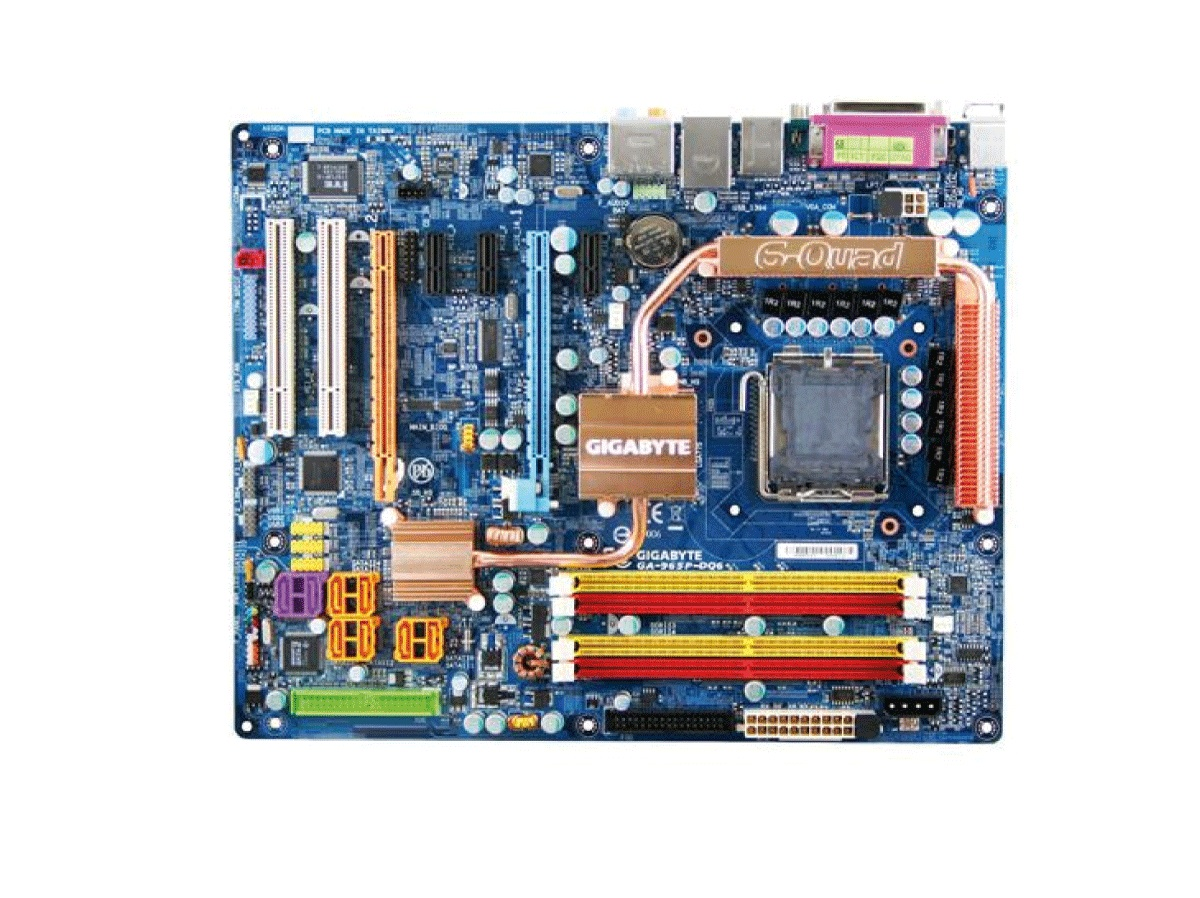
\includegraphics[width=.75\linewidth]{img/s01/carte_mere_commentee_1.jpg}}%
    \only<2|handout:1>{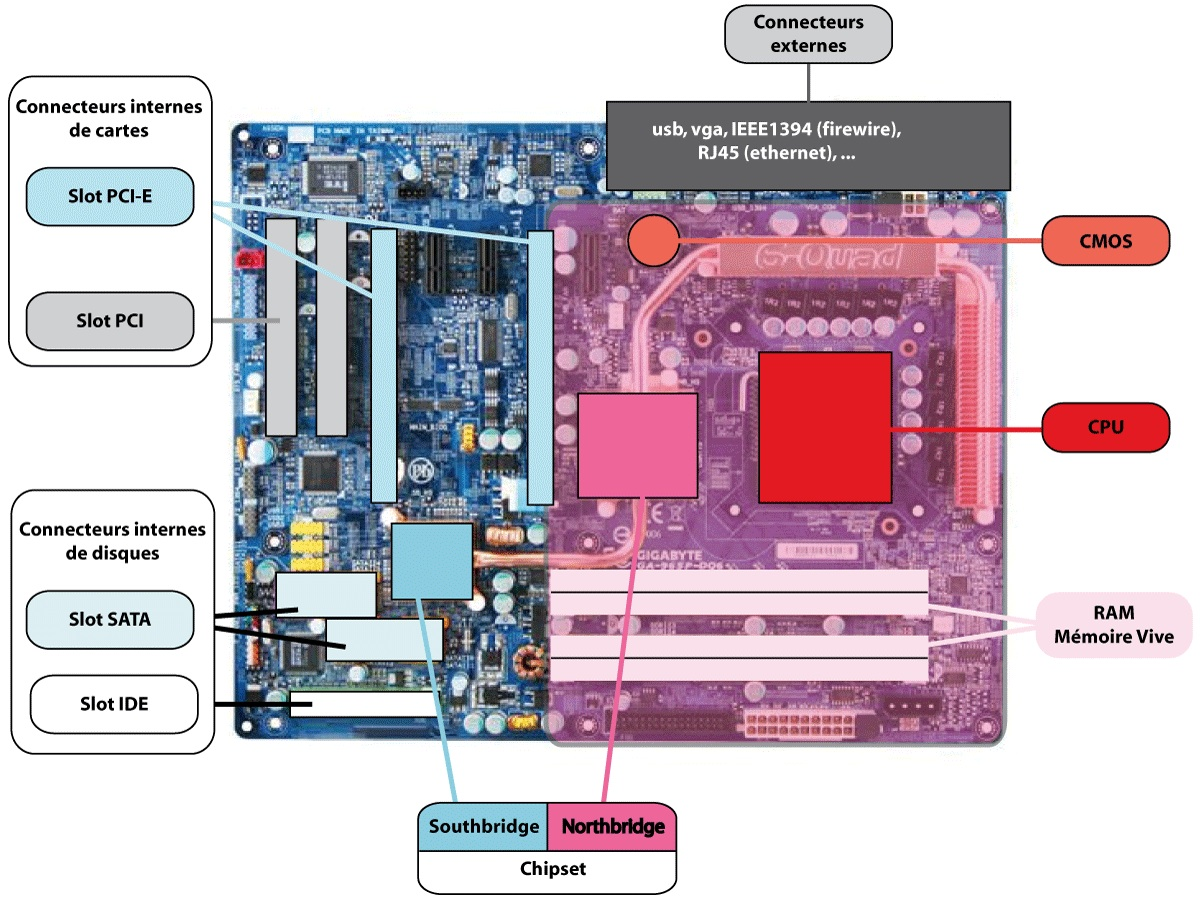
\includegraphics[width=.75\linewidth]{img/s01/carte_mere_commentee_2.jpg}}%
  }

  La carte mère est l'élément central de l'ordinateur sur lequel sont
  assemblés et mis en relation tous les composants matériels. Elle
  permet à tous ses composants de fonctionner ensemble efficacement.
\end{frame}

\begin{frame}{Les unités de calcul}
  \center 
\includegraphics[height = 3 cm]{img/s01/CPU.png}
  \begin{block}{CPU - Central Processing Unit}
    \begin{itemize}
    \item C'est une puce qui traite des instructions élémentaires en
      réalisant des calculs binaires,
    \item Fréquence de l'ordre de 3 GHz.
    \end{itemize}
  \end{block}
  \begin{block}{GPU - Graphics Processing Unit}
    C'est une puce placée sur les cartes graphiques
    \begin{itemize}
    \item Elle prend en charge les nombreux calculs de rafraichissement
      des images 3D
    \item Une carte graphique moderne peut compter une grande quantité
      de ces puces.
    \end{itemize}
  \end{block}
\end{frame}

\begin{frame}{Des mémoires différentes pour des usages différents}
  \begin{columns}
    \only<1|handout:1>{
      \begin{column}{.65\linewidth}
        \begin{block}{ROM : Read Only Memory}
          \begin{itemize}
          \item Mémoire non-volatile maintenue par une conception
            physique,
          \item Taille limitée car très chère, très rapide,
          \item Contient instructions d'amorçage, routines\dots
          \end{itemize}
        \end{block}
        \begin{block}{RAM : Random Access Memory}
          \begin{itemize}
          \item Mémoire volatile: maintenue par une tension électrique,
          \item Accès rapide,
          \item Taille limitée car assez chère.
          \end{itemize}
        \end{block}
        \begin{block}{Disque Dur, clef-usb, \dots}
          \begin{itemize}
          \item Mémoire non-volatile (enregistrement magnétique le plus
            souvent),
          \item Accès lent,
          \item Taille très grande (support de stockage de masse),
            beaucoup moins chère.
          \end{itemize}
        \end{block}
      \end{column}
    } \only<2|handout:2>{ 
      \begin{column}{.65\linewidth}
        \begin{block}{Organisation de la mémoire}
          Les ordinateurs réalisent des calculs logiques sur des données
          binaires\
          \begin{itemize}
          \item Les données et les instructions sont stockées sous forme
            de blocs repérés par une adresse,
          \item Les blocs contiennent une information binaire organisée
            en octet. Chaque octet contient 8 bits d'information qui
            sont lus comme une suite ordonnée de 0 ou de 1 ou de Vrai et
            de Faux.
          \item Un octet peut prendre $2^8=256$ valeurs différentes.
          \end{itemize}
        \end{block}
        \centerline{\includegraphics[height=3cm]{img/s01/Memoire.jpg}}
      \end{column}
    }%
    \begin{column}{.3\linewidth}
      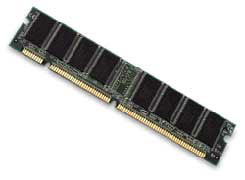
\includegraphics[width=\linewidth]{img/s01/RAM.png}\\
      \vspace{1cm}
      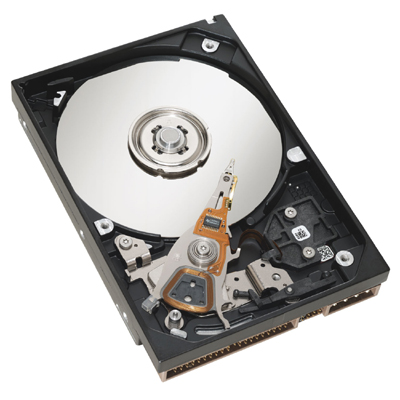
\includegraphics[width=\linewidth]{img/s01/disque_dur.png}
    \end{column}
  \end{columns}
\end{frame}
\begin{frame}{Les périphériques}
  \begin{block}{Des composants externes}
    En fonction de leur tâche, de nombreux composants \textit{ad hoc}
    peuvent être \textit{greffés} sur la structure de base précédemment
    décrite. Par exemple:
    \begin{itemize}
    \item Ordinateur de Maison: Écran, souris, imprimante, scanner,
      joystick, modem, \dots
    \item Ordinateurs de bord: Sondes, actioneurs, \dots
    \item Télephone: Antenne, récepteurs, \dots
    \item Robot médical: Interface haptique, bras mécaniques, \dots
    \end{itemize}
  \end{block}
  \begin{block}{Des composants internes}
    En fonction des possibilités des cartes mères plusieurs types de
    composants peuvent être ajoutés:
    \begin{itemize}
    \item Cartes vidéo, Cartes son, disques durs internes, lecteurs,
      \dots
    \item Cartes d'acquisition ou de pilotage de périphériques, \dots
    \end{itemize}
  \end{block}
  \begin{center}
    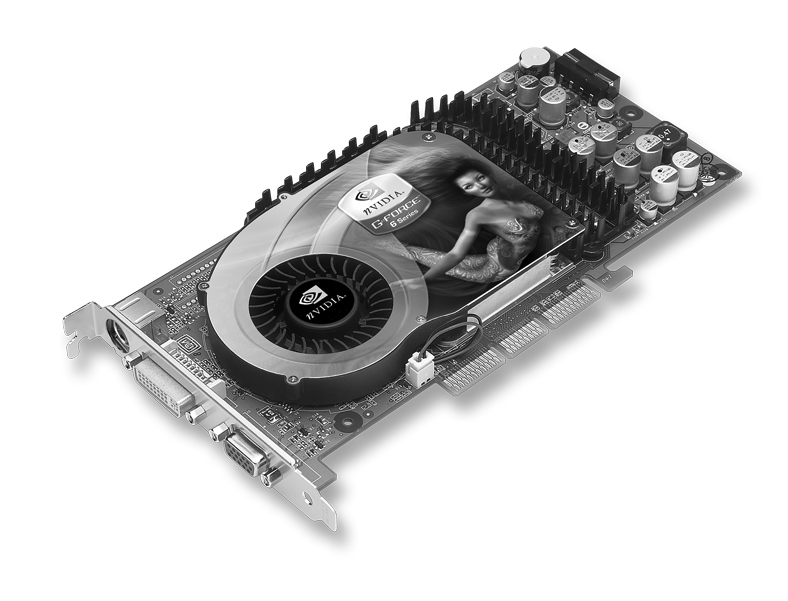
\includegraphics[height=2cm]{img/s01/carte_video.png}
    \hspace{2cm}
    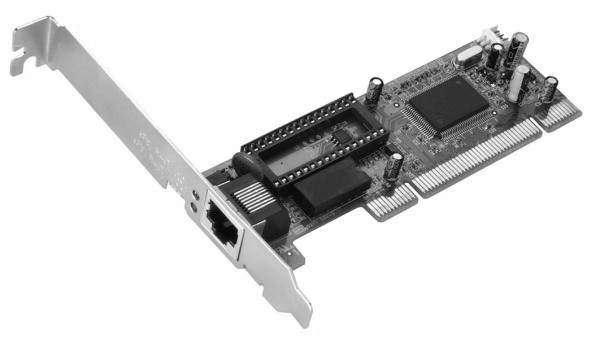
\includegraphics[height=2cm]{img/s01/carte_reseau.png}
  \end{center}
\end{frame}

\begin{frame}{Les bus}
  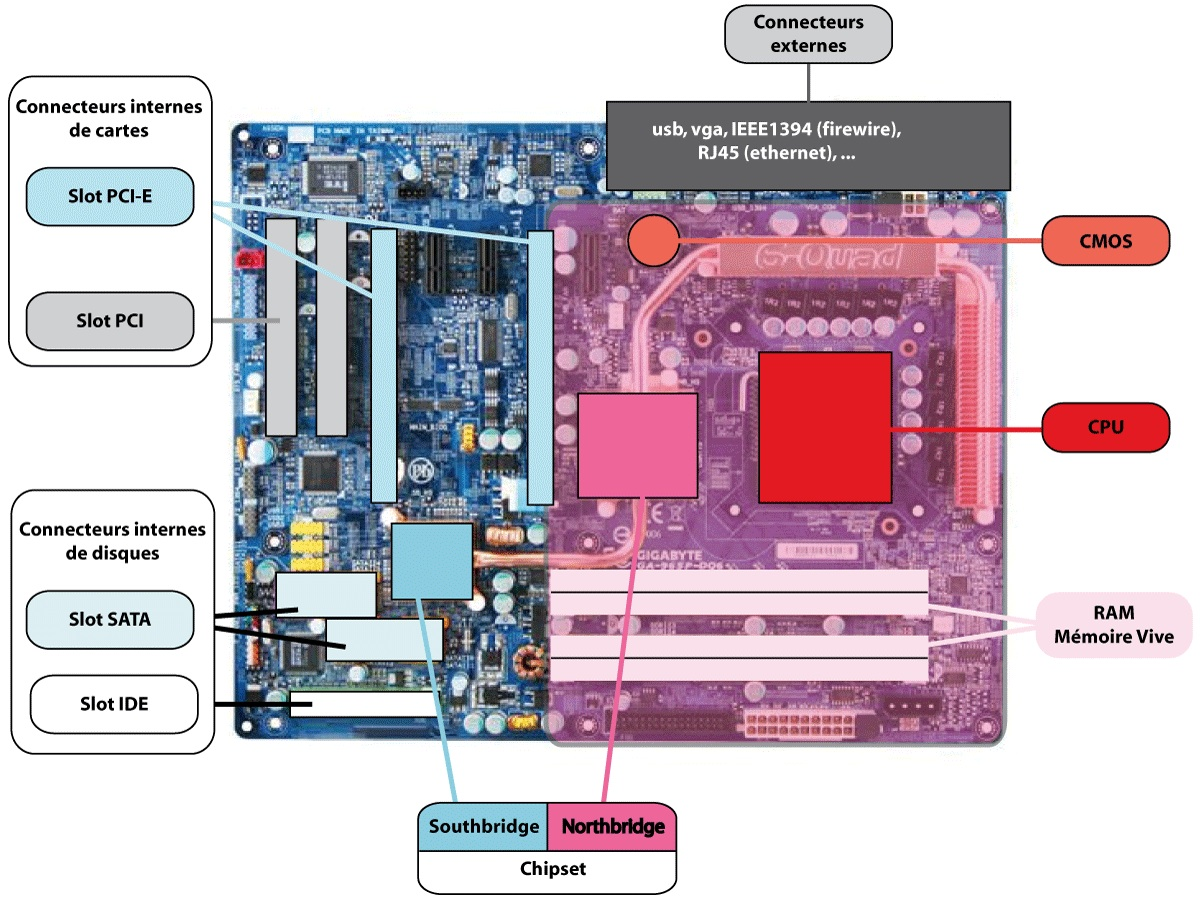
\includegraphics[width=6cm]{img/s01/carte_mere_commentee_2.jpg}%
  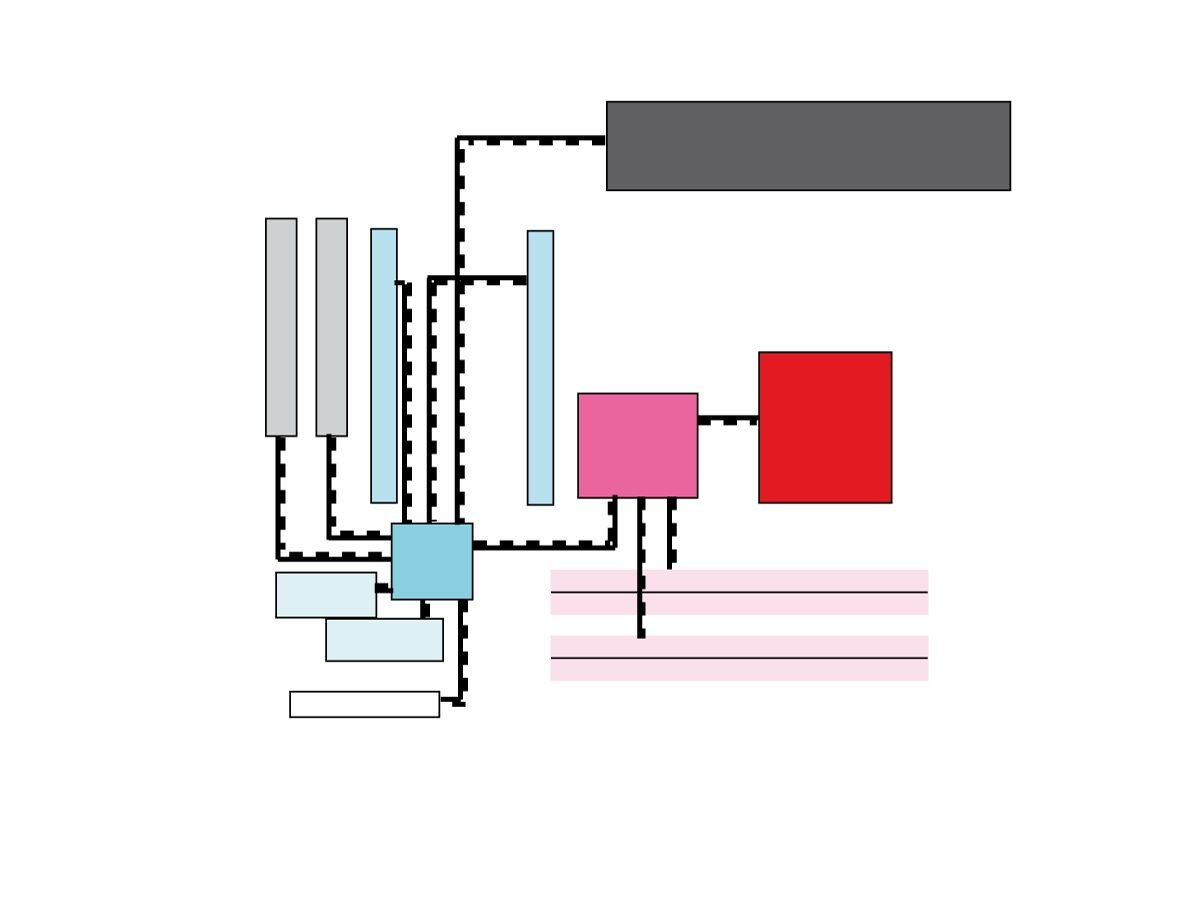
\includegraphics[width=6cm]{img/s01/carte_mere_commentee_3.jpg}%
  \begin{block}{La carte mère intègre les bus.}
    \begin{itemize}
    \item Les bus sont des unités physiques qui assurent le transport
      efficace de l'information entre les différents composants
      connectés à la carte mère,
    \item La largeur (8, 16, 32 64 bits), série ou parallèle et la
      fréquence ($10^2-10^3$ MHz) des bus règlent le débit d'information
      entre les composants. Cela conditionne donc fortement l'efficacité
      d'une configuration matérielle.
    \end{itemize}
  \end{block}
\end{frame}


% Local Variables:
% TeX-master: "sys01"
% TeX-PDF-mode: t
% fill-column: 78
% coding: utf-8-unix
% mode-require-final-newline: t
% mode: latex
% mode: flyspell
% ispell-local-dictionary: "francais"
% End:

\section{Organiser ses données}
\subsection{Les fichiers : noms et contenu}
\begin{frame}{Un fichier}
  \begin{block}{De l'information au stockage}
    Les informations utilisées dans un ordinateur sont stockées dans la
    \emph{mémoire de masse}, qui se distingue de la \emph{mémoire vive}
    par sa résistance à l'extinction et de la \emph{mémoire morte} (et
    plus tard, du \emph{firmware}) par sa mutabilité.

    Les performances des systèmes de stockage de masse sont meilleures
    chaques années, mais l'ordre de grandeur reste la ms ou 100 µs.
  \end{block}
  \begin{block}{De l'information au fichier}
    L'information est découpée en petites unités qui s'appellent des
    fichiers, sémantiquement cohérentes --- ce sont des informations qui
    « vont ensemble ». Ces éléments de base du stockage informatique
    peuvent ne contenir que très peu d'information ou représenter
    plusieurs Go de données par fichier.

    Un fichier est lié à la façon dont on y accède (son \emph{nom} et
    son \emph{chemin}), mais nous verrons que ce n'est pas un
    identifiant : il peut y avoir plusieurs accès différents à un même
    fichier (\emph{liens}).
  \end{block}
\end{frame}
\begin{frame}{Noms et contenu des fichiers}
  \begin{block}{La décomposition traditionnelle d'un nom de fichier}
    \begin{columns}
      \begin{column}{8cm}
        Deux parties séparées par un point:
        \begin{itemize}
        \item La $1\up{ère}$ partie informe sur la nature du contenu du
          fichier,
        \item La $2\up{ème}$ partie informe sur le format ou la finalité des données.
        \end{itemize}
      \end{column}
      \begin{column}{3cm}
        \begin{tabular}{|r@{}r@{}l|}
          \hline
          {\color{solarizedRed}nom}&.&{\color{solarizedGreen}extension} \\
          {\color{solarizedRed}prefix}&.&{\color{solarizedGreen}suffix} \\
          {\color{solarizedRed}description}&.&{\color{solarizedGreen}format}\\
          \hline
        \end{tabular}
      \end{column}
    \end{columns}
    \begin{itemize}
    \item[\ddialogwarning] Selon les systèmes, certains caractères sont interdits. Par exemple \texttt{*} sous Windows, \texttt{/} sous Linux.
    \end{itemize}
  \end{block}
  \begin{columns}
    \begin{column}{5.5cm}
      \begin{block}{Exemples de noms de fichiers}
        \begin{center}
          \begin{tabular}{ll}
            \hline
            Extension&Contenu\\
            \hline
            .c&Sources C\\
            .html&Document Web\\
            .pdf&Document Mis en page\\
            .txt&Texte brut\\
            \hline
          \end{tabular}
          \vfill
          \begin{tabular}{ll}
            \hline
            Enigmatique&Informatif\\
            \hline
            e3.c&teste\_boucle\_for.c\\
            New.pdf&2011\_IntroSys\_cours\_1.pdf\\
            toto.sh&test\_boucle\_for.sh\\
            \hline
          \end{tabular}
        \end{center}
      \end{block}
    \end{column}
    \begin{column}{5.5cm}
      \begin{alertblock}{Choix des noms}
        \begin{itemize}
        \item[\ddialoginformation] Ils doivent être choisis minutieusement pour être informatifs.
        \item[\ddialogsystem] Choisir un nom : réfléchir pour un gain de temps pour
          retrouver le fichier ou le répertoire concerné.
        \item[\ddialogwarning] Importance de la casse (Linux), tolérance
          ailleurs (OS X, Windows).
        \end{itemize}
      \end{alertblock}
    \end{column}
  \end{columns}
\end{frame}
\subsection{Organisation des données enregistrées}
\begin{frame}{Des fichiers et des répertoires}
  \begin{block}{Les fichiers... en vrac ?}
    Les fichiers sont regroupés dans des répertoires (en anglais
    \emph{directory} ou \emph{folders}). Les répertoires peuvent
    contenir des fichiers ou d'autres répertoires. L'organisation des
    fichiers est réglée par le \emph{système de fichiers}
    (ang. \emph{filesystem}).

    \begin{itemize}
    \item Cette organisation arborescente permet de faciliter la
      recherche d'un fichier,
    \item Les fichiers sont regroupés par application, par thème, par
      format, par fonction, \dots
    \item Organisation \emph{hiérarchique} qui permet d'organiser les données et
      de faciliter leur accès.
    \end{itemize}
  \end{block}
  \begin{columns}
    \begin{column}{.7\linewidth}
      \begin{block}{De très nombreux fichiers et répertoires}
        \begin{itemize}
        \item[\ddialoginformation] Le nombre de fichiers enregistrés sur un disque dur peut
          aisément dépasser 100.000 fichiers,
        \item Dans un même répertoire le nom est un identifiant.
        \item Les répertoires et les fichiers partagent les mêmes noms.
        \item[\dialogwarning] Sous Windows, pas d'extension pour les répertoires.
        \end{itemize}
      \end{block}
    \end{column}%
    \begin{column}{.25\linewidth}
      % 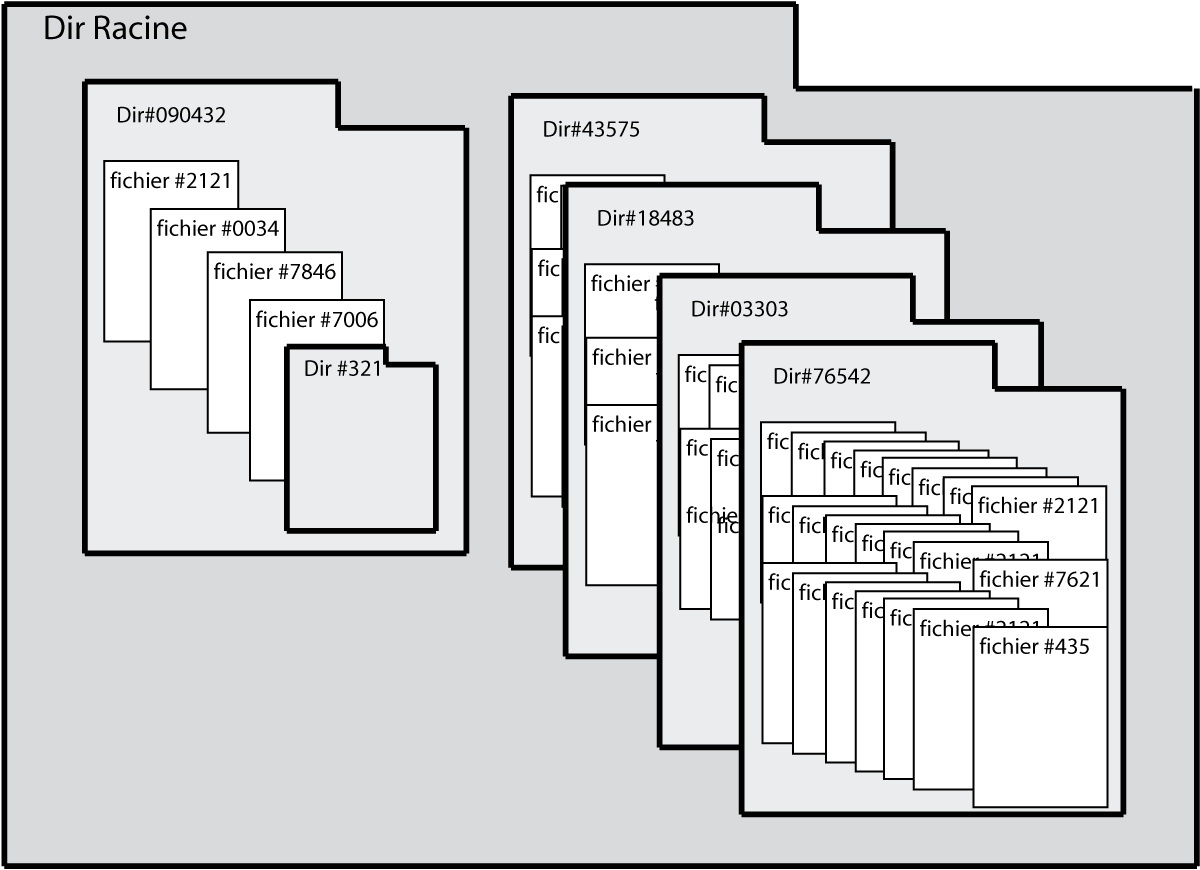
\includegraphics[width=\linewidth]{img/s02/file_system}
      \begin{alertblock}{Remarque}
        \begin{itemize}
        \item[\dialogerror] Avec tous les fichiers au même
          \textit{endroit}, il est très difficile de les lister (trop à
          lire).
        \end{itemize}
      \end{alertblock}
    \end{column}
  \end{columns}
\end{frame}

\subsection{L'organisation arborescente}
\begin{frame}{Exemple d'arborescence Linux}
  \dirtree{%
    .1 \DTd{}\DTfcomment{Répertoire racine \emph{(Root Directory)}}.  .2
    \DTd{bin}.  .3 (\dots).  .2 \DTd{home}.  .3
    \DTd{moi}\DTfcomment{Répertoire personnel \emph{(User
        directory)}}.  .4 \DTd{Mes~Documents}.  .5 ListeDesCourses.txt.
    .5 Exercice\_1.sh.  .4 (\dots).  .3 \DTd{anonymous}.  .4
    LisezMoi.txt.  .4 \DTd{Telechargements}.
    % .5 Cours\_Systeme.pdf.
    .5 (\dots).  .2 (\dots).  }
  \begin{alertblock}{Les répertoires importants}
    \begin{itemize}
    \item La \textbf{racine} (\textit{Root directory}) contient tous
      les répertoires et fichiers accessibles depuis le système.
    \item Le \textbf{répertoire personnel} (\textit{User Directory} ou
      \textit{Home Directory}) est le répertoire dans lequel
      l'utilisateur peut faire ce qu'il veut (écrire, modifier,
      supprimer, installer \dots).
    \end{itemize}
  \end{alertblock}
\end{frame}
\subsection{La notion de chemin}
\begin{frame}{La notion de chemin}
  \begin{block}{Le chemin définit un accès unique à partir de la racine}
    \begin{itemize}
    \item Deux fichiers ou répertoires ne peuvent pas porter le même nom
      si ils sont dans un même répertoire.
    \item Sous Linux, les noms des fichiers et répertoires différencient
      les caractères \textsc{Majuscules} et minuscule. Les fichiers
      \alert{E}ssai.txt et \alert{e}ssai.txt peuvent donc être dans le
      même répertoire.
    \end{itemize}
  \end{block}
  \begin{block}{Exemples de chemins absolus}
    \dirtree{%
      .1 \DTd{}\DTfcomment{Un chemin absolu part de la racine {\color{solarizedAccent}/}}.
      .2 \DTd{home}\DTfcomment{/{\color{solarizedAccent}home/}}.
      .3 \DTd{moi}\DTfcomment{/home/{\color{solarizedAccent}moi/}}.
      .4 \DTd{Etoiles}\DTfcomment{/home/moi/{\color{solarizedAccent}Etoiles/}}.
      .5 SOLEIL.jpg\DTfcomment{/home/moi/Etoiles/{\color{solarizedAccent}SOLEIL.jpg}}.
      .5 Soleil.jpg\DTfcomment{/home/moi/Etoiles/{\color{solarizedAccent}Soleil.jpg}}.
      .4 \DTd{Systeme\_Solaire}\DTfcomment{/home/moi/{\color{solarizedAccent}Systeme\_Solaire/}}.
      .5 SOLEIL.jpg\DTfcomment{/home/moi/Systeme\_Solaire/{\color{solarizedAccent}SOLEIL.jpg}}.
    }
  \end{block}
  \begin{alertblock}{Syntaxe d'un chemin absolu}
    Le chemin \textit{absolu} d'un élément du système de fichier est
    unique (sauf avec un \emph{lien}). Il donne la liste des répertoires
    et sous-répertoires en partant de la racine \lin{/} (la référence de
    l'arborescence) jusqu'à la cible.
  \end{alertblock}
\end{frame}

% MOVE TO 03
% \begin{frame}{La notion de partition}
%   \begin{block}{Windows : les partitions visibles}
%     Le ou les disques sont découpés en systèmes de fichiers indépendants
%     qui sont numérotés par des lettres. A et B sont réservés au lecteur
%     de disquette, C au disque système. Nombre limité de partitions.

%     Les partitions aident à l'organisation des données par type
%     (système, utilisateurs, sauvegarde).
%   \end{block}
%   \begin{block}{Unix : les partitions invisibles}
%     Sous Unix et ses variantes (OS X et Linux), la partition racine est
%     celle qui contient le système. Les autres partitions sont
%     \emph{montées} à la place d'un répertoire et sont en quelque sortes
%     greffées dans l'arbre qui reste unique. La racine de la partition
%     montée prend la place du répertoire dans l'arborescence.
%   \end{block}
% \end{frame}

\subsection{Répertoire courant et chemins relatifs}
\begin{frame}{Répertoire courant et chemins relatifs}
  \begin{block}{Le répertoire courant}
    \begin{itemize}
    \item Le répertoire courant est un répertoire de référence d'où sont
      lancées les commandes du shell.
    \item Par défaut, le répertoire courant est le répertoire personnel
      de l'utilisateur,
    \item Naviguer dans l'arborescence équivaut à modifier le répertoire
      courant.
    \end{itemize}
  \end{block}
  \begin{block}{Exemples de chemins relatifs}
    \dirtree{%
      .1 \DTd{home}\DTfcomment{../..}.
      .2 \DTd{moi}\DTfcomment{../}.
      .3 \DTd{Etoiles}\DTfcomment{{\color{solarizedRed}Répertoire Courant ~~./}}.
      .4 SOLEIL.jpg\DTfcomment{SOLEIL.jpg {\color{black}ou} ./SOLEIL.jpg}.
      .4 Antares.jpg\DTfcomment{Antares.jpg {\color{black}ou} ./Antares.jpg}.
      .3 \DTd{Systeme\_Solaire}\DTfcomment{../Systeme\_Solaire/}.
      .4 terre.gif\DTfcomment{../Systeme\_Solaire/terre.gif}.
    }
  \end{block}
  \begin{alertblock}{Syntaxe d'un chemin relatif}
    \begin{itemize}
    \item Le chemin \textit{relatif} d'un fichier ou d'un répertoire donne la liste des répertoires et sous-répertoires en partant du répertoire courant (la référence \textit{relative} dans l'arborescence) jusqu'à la cible.
    \item Il est relatif, car lorsque le répertoire courant change, le chemin relatif change.
    \end{itemize}
  \end{alertblock}
\end{frame}
% MOVE TO 03
% \begin{frame}{Chemin canonique}
%   \begin{block}{Chemin canonique}
%     Le chemin qui part de la racine et n'emprunte aucun \emph{lien symbolique} (une forme de lien que nous verrons plus loin) ni aucun \emph{lien parent} (raccourci \lin{..} vers un répertoire parent d'un autre) est appelé le chemin \emph{canonique absolu}.
%   \end{block}
% \end{frame}
%%%%%%%%%%%%%% 
\subsection{Notation spéciales}
\begin{frame}{Notation spéciales}
  \begin{block}{Les chemins des répertoires de référence}
    \begin{columns}
      \begin{column}{6cm}
        \begin{center}
          \begin{tabular}{lr}
            \hline
            Répertoire&Notation\\
            \hline
            Répertoire racine&\lin{/}\\
            Répertoire personnel&\lin{\~{}}\\
            \hline
          \end{tabular}
        \end{center}
      \end{column}
      \begin{column}{6cm}
        \begin{center}
          \begin{tabular}{lr}
            \hline
            Répertoire&Notation\\
            \hline
            Répertoire courant&\lin{.}\\
            Répertoire parent&\lin{..}\\
            \hline
          \end{tabular}
        \end{center}
      \end{column}
    \end{columns}
    \begin{itemize}
    \item[\ddialogwarning] La notation \lin{\~{}} est un chemin
      absolu, remplacée par le vrai chemin avant l'exécution des
      commandes. C'est un raccourci \emph{au niveau du shell, pas au
        niveau du système d'exploitation}.
    \end{itemize}
  \end{block}
  \begin{block}{Exemple de chemins valides pointant le fichier cible}
    \begin{columns}
      \begin{column}{55mm}
        \dirtree{%
          .1 \DTd{}\DTfcomment{{\color{solarizedAccent}Répertoire Racine}}.
          .2 \DTd{home}.
          .3 \DTd{moi}\DTfcomment{{\color{solarizedAccent}Répertoire Personnel}}.
          .4 \DTd{Etoiles}\DTfcomment{{\color{solarizedAccent}Répertoire Courant}}.
          .5 Soleil.jpg\DTfcomment{Fichier cible}.
        }
      \end{column}
      \begin{column}{7cm}
        \begin{center}
          \footnotesize{
            \begin{tabular}{l}
              \hline
              Chemins Absolus\\
              \hline
              \lin{/home/moi/Etoiles/Soleil.jpg}\\
              \lin{\~{}/Etoiles/Soleil.jpg}\\
              \lin{/home/moi/../moi/Etoiles/Soleil.jpg}\\
              \lin{/home/moi/../../home/moi/Etoiles/Soleil.jpg}\\
              \hline
              Chemins Relatifs\\
              \hline
              \lin{Soleil.jpg}\\
              \lin{./Soleil.jpg}\\
              \lin{../Etoiles/Soleil.jpg}\\
              \lin{../../moi/Etoiles/./Soleil.jpg}\\
            \end{tabular}
          }
        \end{center}
      \end{column}
    \end{columns}	
  \end{block}
\end{frame}

\begin{frame}{L'archivage}
  \begin{block}{D'une arborescence à un fichier}
    Une technique souvent utilisée consiste à transformer une partie de
    l'arborescence en un fichier qui n'est pas utilisable directement. Ce
    fichier peut ensuite être retransformé en une arborescence.
  \end{block}
  \begin{columns}
    \begin{column}{55mm}
      \begin{block}{Le format tar}
        Utilisé depuis les années 80, le format tar est un pilier du
        monde Unix. Il est parfaitement libre. Il servait initialement
        aux sauvegardes sur bande magnétique (\emph{t}ape
        \emph{ar}chive).
        
        Le format tar ne permet pas la compression, mais la commande
        \lin{tar} donne accès à des programmes de compression qui
        permettent de réduire la taille de l'archive. Une archive au
        format tar est appelée un(e) \emph{tarball}.

        Le compresseur le plus connu est \lin{gzip} dont les fichiers
        compressés ont un suffixe \lin{.gz}. Souvent on combine les deux
        suffixes : une archive compressée peut ainsi s'appeler
        \lin{textes2015.tar.gz} ou \lin{textes2015.tgz}.
      \end{block}
    \end{column}
    \begin{column}{55mm}
      \begin{block}{Le format zip}
        Principalement utilisé pour son universalité depuis 1986, le format zip est
        plus ou moins libre (il y a des doutes sur la possibilité de
        brevet sur les techniques employées). Le format zip n'est pas
        uniquement caractérisé par son extension : plusieurs autres
        formats de fichier sont en fait une archive ZIP qui contient
        divers documents (par exemple, un fichier \lin{docx} pour
        Microsoft Word est en fait un ZIP qui contient divers fichiers
        XML et images).

        Le format zip, en plus de l'archivage permet aussi la
        compression. La commande \lin{zip}/\lin{unzip} doit donc
        permettre la décompression.
      \end{block}
    \end{column}
  \end{columns}
\end{frame}

\subsection{Quelques mini-manuels}
\begin{frame}{Conventions}
  \begin{block}{Noms et chemins}
    \begin{itemize}
    \item Un chemin peut être absolu ou relatif. Il peut utiliser les notations spéciales.
    \item Par convention la notion de fichier sera comprise dans son sens large. Par exemple, le chemin d'un fichier devra être interprété sans distinction comme le chemin vers un fichier ordinaire ou comme le chemin vers un répertoire (sauf mention contraire explicite).
    \end{itemize}
  \end{block}
  \begin{block}{Commandes, options, paramètres}
    \begin{description}
    \item[Commande] c'est le nom d'un programme qui exécute une action.
    \item[Options] ce sont des paramètres optionnels. Ils peuvent être
      omis. L'ajout d'options modifie le comportement de la commande (le
      résultat). Les options sont montrées encadrées par les caractères
      \lin{[ ... ]} (qu'il ne faut pas mettre).
    \item[Paramètres] ce sont des arguments que la commande évalue.
    \end{description}
  \end{block}
  \begin{block}{Sources et destination}
    Les commandes de déplacement acceptent une ou des \emph{sources} qui
    sont des fichiers ou répertoires d'origine, et une
    \emph{destination} qui est un fichier ou un répertoire.
  \end{block}
\end{frame}
\begin{frame}{Manipulation de l'arborescence en ligne de commande}
  \begin{columns}
    \begin{column}{4cm}
      \begin{block}{Alternatives pour naviguer dans l'arborescence et
          manipuler les fichiers}
        \begin{center}
          Interface Graphique\\
          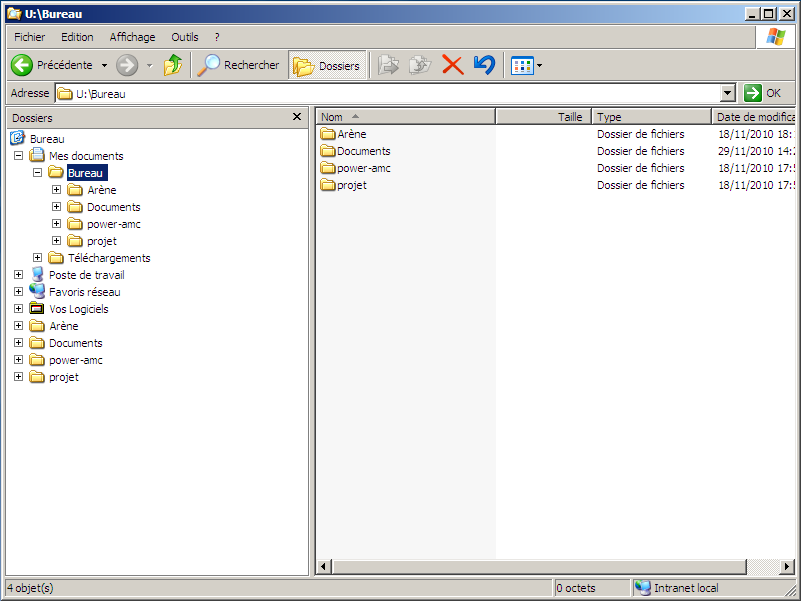
\includegraphics[height=2cm]{img/s02/explorer_windows.png}
        \end{center}
        \begin{center}
          Ligne de Commande\\
          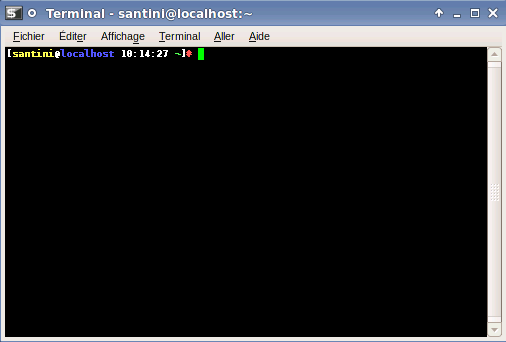
\includegraphics[height=2cm]{img/s02/terminal_single.png}
        \end{center}
      \end{block}
    \end{column}
    \begin{column}{75mm}
      \begin{block}{Boîte à outils : manipuler l'arborescence}
        \begin{center}
          \begin{tabular}{ll}
            \hline
            Commande&Fonction principale\\
            \hline
            \lin{pwd}&Afficher le nom du répertoire courant\\
            \lin{cd}&Changer de répertoire courant\\
            \lin{ls}&Afficher le contenu d'un répertoire\\
            \lin{cat}&Afficher le contenu d'un fichier\\\hline
            \lin{touch}&Créer un fichier\\
            \lin{mkdir}&Créer un répertoire\\\hline
            \lin{rm}&Supprimer fichier(s) ou répertoire(s) \\
            \lin{cp}&Copier fichier(s) ou répertoire(s)\\
            \lin{mv}&Déplacer/Renommer fichier(s) ou répertoire(s)\\
            \hline
          \end{tabular}
        \end{center}
      \end{block}
    \end{column}
  \end{columns}
\end{frame}
\manpage{pwd} \manpage{cd}
\manpage{ls} \manpage{ls(bis)} \manpage{cat}
\manpage{touch} \manpage{mkdir} \manpage{mkdir(bis)}
\manpage{rm} \manpage{rm(bis)} \manpage{cp}
\manpage{cp(bis)} \manpage{cp(ter)} \manpage{mv} \manpage{mv(bis)}
\manpage{mv(ter)}
\manpage{tar}\manpage{tar(bis)}

\begin{exercice}
  \begin{exercicelet}{Préparation}
    \begin{questions}
    \item Ouvrez un terminal. Vérifiez que le répertoire dans lequel
      vous êtes est bien \lin{/home/usager/123456789/}. Quelle est la
      commande qui permet de le faire ? (123456789 = votre identifiant)
    \item Vérifiez le contenu du répertoire \lin{Documents} qui est dans
      votre répertoire personnel. Quelle est la commande qui permet de
      le faire ? Est-ce qu'il y a quelque chose ?
    \item Faites la vérification de trois façons différentes : chemin
      absolu, utilisation du raccourci \lin{\~}, utilisation d'un chemin
      relatif.
    \item Changez le répertoire courant pour aller dans
      \lin{Documents}. Quelle est la commande pour le faire ?
    \item Créez en ligne de commande un répertoire \lin{m1101} dans
      \lin{{\textasciitilde}/Documents}. À partir de maintenant, assurez-vous que le
      répertoire courant est ce répertoire \lin{m1101}.
    \item Téléchargez l'archive contenant les données pour ce TP:
      Allez sur la page
      \url{http://lipn.fr/~dubacq/m1101.html}.
      Téléchargez le fichier \lin{photos.tar}. Recherchez où
      le fichier a été écrit dans l'arborescence de votre répertoire
      personnel.
    \item Donnez la (suite de) commande(s) permettant de déplacer le
      fichier d'archive dans le répertoire \lin{m1101} que vous venez de
      créer. À la fin des commandes, le répertoire \lin{m1101} sera
      toujours votre répertoire courant et ne contiendra que le fichiers
      photos.tar.
    \item Quelle commande permet de vérifier que l'archive est bien dans
      le répertoire \verb|~/Documents/m1101|?
    \end{questions}
  \end{exercicelet}
\end{exercice}
\begin{exercice}
  \begin{exercicelet}{Examen de fichiers}
    \begin{questions}
    \item Quelles sont les informations données par le nom du fichier?
    \item\label{qsee} Les commandes \texttt{less}, \texttt{cat} et \texttt{hexdump} permettent
      d'afficher le contenu d'un fichier. Analysez la différence de
      comportement entre ces deux commandes sur le fichier
      \lin{photos.tar}. Qu'en concluez-vous? Quel est le programme le
      plus adapté pour voir le contenu de ce fichier ?
      \begin{correction}
        cat affiche brutalement du binaire sans filtrer
        (incompréhensible), less propose une interface (mais ça reste du
        binaire dans la configuration par défaut de Debian), hexdump
        transforme le binaire en hexadécimal (ce n'est pas beaucoup plus
        lisible). Le programme le plus adapté est donc... tar, comme
        montré dans la question suivante ! Avec \texttt{tar tf
          photos.tar} on obtient la liste des fichiers.
      \end{correction}
    \item Relisez le manuel de la commande \texttt{tar}. Vérifiez la
      liste des fichiers contenus dans l'archive. Combien y en a-t-il ?
    \item Sortez les fichiers de l'archive.
      \begin{correction}
        tar xf photos.tar
      \end{correction}
    \item Avec les commandes de la question~\ref{qsee}, regardez le
      fichier contenu dans un répertoire. Analysez la différence de
      comportement entre ces commandes. Qu'en concluez-vous?
      \begin{correction}
        La commande less est plus adaptée (pagination, arrêt par la
        touche q). La commande hexdump continue de produire de
        l'hexadécimal (on peut montrer hexdump -C aux curieux).
      \end{correction}
    \end{questions}
    
    Remarques: si un affichage prend trop de temps, utilisez le
    raccourci clavier adéquat pour suspendre l'exécution de la commande
    courante.  Si l'affichage de votre terminal est durablement
    perturbé, dans le menu Terminal \textrightarrow Réinitialiser le
    terminal.
  \end{exercicelet}
\end{exercice}
\subsection{Métacaractères}
\begin{frame}{Le métacaractère \lin{*}}
  \begin{block}{Le caractère \lin{*}}
    \begin{itemize}
    \item[\ddialogsystem] Le shell traduit la ligne de commande en \texttt{commande argument1
        argument2 ...}. Avant l'exécution, il traduit certains caractères
      selon des règles précisées ici.
    \item Le cataractère \lin{*} est utilisé comme un \textit{joker}
      pour remplacer une chaîne de caractères,
    \item Il est utilisé dans un chemin pour pointer plusieurs fichiers
      ou répertoires existants dont le chemin partage un motif commun.
    \item Le caractère \lin{*} peut être n'importe où dans le chemin,
      plusieurs fois si nécessaire.
    \end{itemize}
  \end{block}
  \begin{block}{Exemple de manipulation avec la commande \lin{mv}}
    \scriptsize{
      \begin{columns}
        \begin{column}{6cm}
          \begin{center}
            \mpromptS{%
              \promptS{mv *.jpg Images/}{} }
          \end{center}
        \end{column}
        \begin{column}{6cm}
          Ici, le chemin \lin{*.jpg} pointe tous les fichiers du
          répertoire courant dont le nom se fini par l'extension
          \lin{.jpg}. Il pointe donc les fichiers \lin{etacentauri.jpg}
          et \lin{aldebaran.jpg} et exclue les autres fichiers (ici le
          fichier \lin{alphacentauri.gif}).
        \end{column}
      \end{columns}
      \begin{columns}
        \begin{column}{6cm}
          \dirtree{%
            .1
            \DTd{{\color{solarizedRed}moi}}\DTfcomment{{\color{solarizedRed}Répertoire
                Courant}}.  .2 aldebaran{\color{solarizedGreen}.jpg}
            \DTfcomment{{\color{solarizedGreen}Fichier ciblé}}.  .2
            alphacentauri.gif .  .2
            etacentauri{\color{solarizedGreen}.jpg}
            \DTfcomment{{\color{solarizedGreen}Fichier ciblé}}.  .2
            \DTd{{\color{solarizedBlue}Images}}\DTfcomment{{\color{solarizedBlue}Répertoire
                final}}.  }
        \end{column}
        \begin{column}{6cm}
          \dirtree{%
            .1
            \DTd{{\color{solarizedRed}moi}}\DTfcomment{{\color{solarizedRed}Répertoire
                Courant}}.  .2 alphacentauri.gif .  .2
            \DTd{{\color{solarizedBlue}Images}}\DTfcomment{{\color{solarizedBlue}Répertoire
                final}}.  .3 {\color{solarizedGreen}aldebaran.jpg}
            \DTfcomment{{\color{solarizedGreen}Fichier déplacé}}.  .3
            {\color{solarizedGreen} etacentauri.jpg}
            \DTfcomment{{\color{solarizedGreen}Fichier déplacé}}.  }
        \end{column}
      \end{columns}
    }
  \end{block}
\end{frame}
\begin{frame}{Exemples d'utilisation de l'étoile}
  \begin{block}{Utilisation simple avec la commande \lin{mv}}
    \scriptsize{
      \begin{columns}
        \begin{column}{6cm}
          \begin{center}
            \mpromptS{%
              \promptS{mv al* Images/}{} }
          \end{center}
        \end{column}
        \begin{column}{6cm}
          Ici, le chemin \lin{al*} pointe tous les fichiers du
          répertoire courant dont le nom commence par les caractères
          \lin{al}. Il pointe donc les fichiers \lin{aldebaran.jpg} et
          \lin{alphacentauri.gif} et exclue les autres fichiers (ici le
          fichier \lin{etacentauri.jpg}).
        \end{column}
      \end{columns}
      \begin{columns}
        \begin{column}{6cm}
          \dirtree{%
            .1
            \DTd{{\color{solarizedRed}moi}}\DTfcomment{{\color{solarizedRed}Répertoire
                Courant}}.  .2 {\color{solarizedGreen}al}debaran.jpg
            \DTfcomment{{\color{solarizedGreen}Fichier ciblé}}.  .2
            {\color{solarizedGreen}al}phacentauri.gif
            \DTfcomment{{\color{solarizedGreen}Fichier ciblé}}.  .2
            etacentauri.jpg.  .2
            \DTd{{\color{solarizedBlue}Images}}\DTfcomment{{\color{solarizedBlue}Répertoire
                final}}.  }
        \end{column}
        \begin{column}{6cm}
          \dirtree{%
            .1
            \DTd{{\color{solarizedRed}moi}}\DTfcomment{{\color{solarizedRed}Répertoire
                Courant}}.  .2 etacentauri.jpg .  .2
            \DTd{{\color{solarizedBlue}Images}}\DTfcomment{{\color{solarizedBlue}Répertoire
                final}}.  .3 {\color{solarizedGreen}aldebaran.jpg}
            \DTfcomment{{\color{solarizedGreen}Fichier déplacé}}.  .3
            {\color{solarizedGreen}alphacentauri.gif}
            \DTfcomment{{\color{solarizedGreen}Fichier déplacé}}.  }
        \end{column}
      \end{columns}
    }
  \end{block}
  \begin{block}{Utilisation double avec la commande \lin{mv}}
    \scriptsize{
      \begin{columns}
        \begin{column}{6cm}
          \begin{center}
            \mpromptS{%
              \promptS{mv *centauri* JPG/}{} }
          \end{center}
        \end{column}
        \begin{column}{6cm}
          Ici, le chemin \lin{*centauri*} pointe tous les fichiers du
          répertoire courant dont le nom contient la chaîne de
          caractères \lin{centauri}. Il pointe donc les fichiers
          \lin{alphacentauri.gif} et \lin{etacentauri.jpg} et exclue les
          autres fichiers (ici le fichier \lin{aldebaran.jpg}).
        \end{column}
      \end{columns}
      \begin{columns}
        \begin{column}{6cm}
          \dirtree{%
            .1
            \DTd{{\color{solarizedRed}moi}}\DTfcomment{{\color{solarizedRed}Répertoire
                Courant}}.  .2 aldebaran.jpg .  .2
            alpha{\color{solarizedGreen}centauri}.gif
            \DTfcomment{{\color{solarizedGreen}Fichier ciblé}}.  .2
            eta{\color{solarizedGreen}centauri}.jpg
            \DTfcomment{{\color{solarizedGreen}Fichier ciblé}}.  .2
            \DTd{{\color{solarizedBlue}Images}}\DTfcomment{{\color{solarizedBlue}Répertoire
                Final}}.  }
        \end{column}
        \begin{column}{6cm}
          \dirtree{%
            .1
            \DTd{{\color{solarizedRed}moi}}\DTfcomment{{\color{solarizedRed}Répertoire
                Courant}}.  .2 aldebaran.jpg .  .2
            \DTd{{\color{solarizedBlue}Images}}\DTfcomment{{\color{solarizedBlue}Répertoire
                final}}.  .3 {\color{solarizedGreen}alphacentauri.gif}
            \DTfcomment{{\color{solarizedGreen}Fichier déplacé}}.  .3
            {\color{solarizedGreen}etcentauri.jpg}
            \DTfcomment{{\color{solarizedGreen}Fichier déplacé}}.  }
        \end{column}
      \end{columns}
    }
  \end{block}
\end{frame}
\begin{frame}{Métacaractère et chemins ciblés}
  \begin{block}{Exemple plus complexe et détails de l'interprétation}
    \begin{itemize}
    \item Le cararctère \lin{*} est développé lors de l'interprétation.
    \end{itemize}
  \end{block}
  \begin{center}
    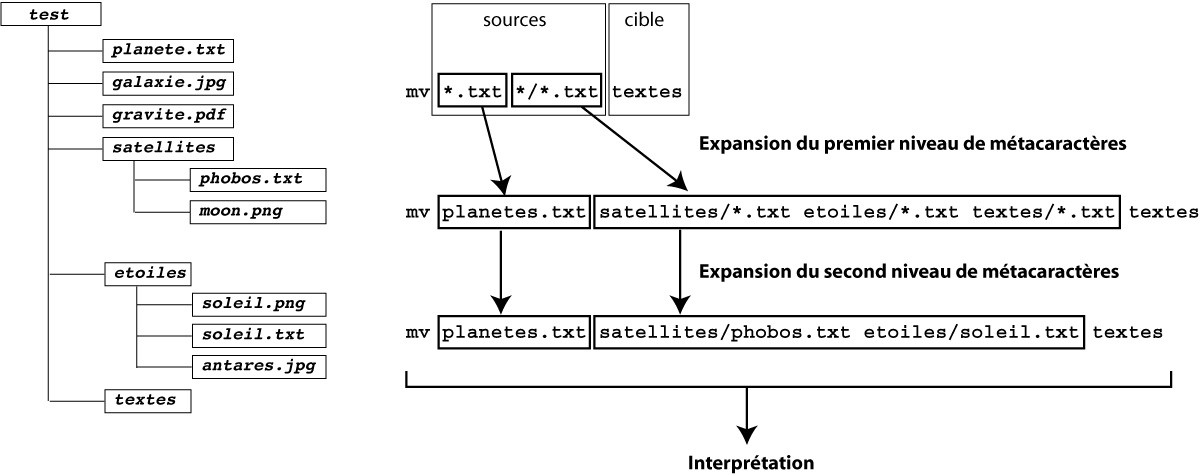
\includegraphics[width=12cm]{img/s02/star_met_mv_interp.jpg}
  \end{center}
\end{frame}
\begin{frame}{Autres métacaractères}
  \begin{alertblock}{Du shell aux programmes}
    Il faut bien se souvenir que les métacaractères sont interprétés par le shell. Cela a deux conséquences :
    \begin{itemize}
    \item Le programme appelé ne sait pas si les noms ont été tapés en entier ou si des métacaractères ont été utilisés. Il n'a que le résultat final.
    \item Dans un programme, on ne peut pas utiliser les métacaractères.
    \end{itemize}
  \end{alertblock}
  \begin{block}{Les jokers}
    Ce sont des motifs simples. Lorsqu'ils ne peuvent pas être
    instanciés, ils ne sont pas supprimés, mais passés tels
    quels. Exemple : \lin{mkdir -p toto/*} selon que \texttt{toto} est
    un répertoire non-vide ou autre chose.

    On y trouve \lin{?} qui remplace une lettre, \lin{[a-c][0-2]} qui remplace a0 b0 c0 a1 b1 c1 a2 b2 c2, 

  \end{block}
  \begin{block}{Les raccourcis}
    Le motif \lin{\{fourch,brou\}ette} est remplacé par
    \lin{fourchette} et \lin{brouette} indépendamment de
    l'existence ou nom de chemins correspondants.
    
    Le motif \lin{\~} a déjà été vu et est remplacé par le chemin absolu
    du répertoire personnel de l'utilisateur courant. \lin{\~{}user} est
    remplacé de la même façon mais pour l'utilisateur \emph{user}.
  \end{block}
\end{frame}
\begin{exercice}
  \begin{exercicelet}{Copie et déplacement}
    \begin{questions}
    \item Quelle commande permet la création "simultanée" de trois
      répertoires \lin{GIF} et \lin{Photos/Portugal},
      \lin{Photos/Marseille} et \lin{Photos/Montagne} ?
    \item Quelle commande permet de \emph{déplacer} depuis le répertoire
      \lin{images} tous les fichiers présentant l'extension
      \lin{gif} dans le répertoire \lin{GIF} nouvellement créé?
    \item Quelle commande permet de \emph{copier} depuis le répertoire
      \lin{images} tous les fichiers présentant l'extension
      \lin{jpg} dans le répertoire \lin{Photos} nouvellement créés?
    \item Définissez le répertoire \lin{Photos/Montagne} comme votre répertoire
      courant. Quelle commande permet de déplacer la photo de chalet dans ce répertoire ?
    \item En vous mettant dans \lin{Photos}, déplacez les photos
      restantes dans le bon répertoire (Marseille est supérieure à
      2000). Si possible, faites usages de jokers.
    \end{questions}
  \end{exercicelet}
\end{exercice}
\begin{exercice}
  \begin{exercicelet}{Suppressions}
    \begin{questions}
    \item Quel est le résultat de la séquence de commandes suivante :
\begin{verbatim}
 cd ..
 rm images
\end{verbatim}
    \item Comment modifier la dernière commande pour supprimer le
      répertoire \texttt{images/}? Comment modifier la commande pour
      éviter les invites de confirmation?
    \item Quelle commande permet de copier le répertoire \texttt{GIF} et
      son contenu dans un répertoire nommé \verb|images_GIF|?
    \item Quelle est la différence entre les deux commandes suivantes:
\begin{verbatim}
      cd ~
      cd /home/usager/votre_identifiant/
\end{verbatim}
    \item Fabriquez une archive qui contient le répertoire Photos (et
      uniquement celui-ci). Vérifiez son contenu.
    \end{questions}
  \end{exercicelet}
  % ----------------limite approximative de cours
\end{exercice}

\subsection{Arborescence et montage}
\begin{frame}{Le partitionnement}
  \begin{block}{Du disque aux partitions}
    \begin{itemize}
    \item Un disque est souvent divisé en plusieurs zones d'usage
      distinct (par exemple, système et données utilisateurs).
    \item Chacun de ces zones est appelée une \emph{partition}. Elle
      est un système de fichiers indépendant des autres, et peut être
      combinée avec d'autres.
    \item Sous Windows, chaque partition est désignée par une lettre
      en fonction de son ordre de découverte par le système. Cette
      lettre fait partie du chemin.
    \item[\dialogwarning] L'ordre des partitions peut changer et donc
      la lettre ; ça pose problème pour les mises à jour.
    \end{itemize}
  \end{block}
  \begin{block}{Montage et démontage}
    \begin{itemize}
    \item Un système d'exploitation peut rendre accessible une
      partition : c'est le \emph{montage} de la partition.
    \item Inversement : c'est le \emph{démontage} de la partition.
    \item[\dialogsystem] Une partition montée peut être utilisée
      normalement par les programmes.
    \item[\dialogerror] Une partition démontée doit utiliser une
      interface spéciale plus compliquée qui contourne le \emph{système
        de fichiers} et permet d'accéder directement au disque.
    \end{itemize}
  \end{block}
\end{frame}
\begin{frame}{Les partitions sous Linux}
  \begin{block}{L'arbre unique}
    \begin{itemize}
    \item Sous Linux, les partitions sont toutes dans regroupés dans une seule arborescence.
    \item[\ddialogsystem] Les partitions qui ne sont pas la racine sont accrochées dans
      la partition racine (ou une autre déjà accrochée) au niveau d'un
      répertoire qui sert de \emph{point de montage}.
    \item[\ddialogerror] Le contenu du point de montage est alors
      inaccessible et remplacé par le contenu du système de fichier qui
      a été monté
    \item Le chemin absolu d'un élément du système monté est le chemin
      du point de montage suivi du chemin dans le système de fichiers
      monté.
    \item[\ddialoginformation] Exemple: fichier \texttt{moi/toto.txt}
      dans un système monté sur \texttt{/home}, le chemin absolu est
      \texttt{/home/moi/toto.txt}.
    \end{itemize}
  \end{block}
  \begin{block}{Le pseudo-système \texttt{/dev}}
    Sous Linux, les périphériques sont accessibles par une interface de
    type fichier. Leur chemin est \texttt{/dev/codeperipherique}. 

    Le sous-arbre à partir de \texttt{/dev} est un système de fichiers
    indépendant d'un périphérique physique. On parle de \emph{système de
      fichiers virtuel}.
  \end{block}
\end{frame}

\manpage{mount}

\begin{exercice}
  \begin{exercicelet}{Analyse de périphériques}
    \begin{questions}
    \item Le périphérique \texttt{zero} est un périphérique virtuel. La
      commande \texttt{dd if=/dev/zero count=1 | hexdump -v} permet de
      voir les 512 premiers octets de ce périphérique virtuel (en
      hexadécimal). Regardez-le. Qu'est-ce qu'il a de particulier ?
      \begin{correction}
        Ce périphérique virtuel n'emet que des octets dont la valeur est
        zéro. Un nombre infini d'octets. L'utilité ne paraît pas très
        évidente, mais ce n'est pas compliqué à faire. Un périphérique
        virtuel est en fait un programme (plus précisément, un morceau
        de ce qu'on appelle le noyau du système d'exploitation) qui
        réagit comme un périphérique, sauf qu'il ne correspond à aucune
        interface physique particulière. Le noyau le considère comme
        s'il existait quelque part un disque infini qui ne contient que
        des zéros.
      \end{correction}
    \item Le périphérique \texttt{urandom} est un périphérique
      virtuel. La commande \texttt{dd if=/dev/urandom count=1 | hexdump
        -v} permet de voir les 512 premiers octets de ce périphérique
      virtuel (en hexadécimal). Regardez-le. Recommencez. Qu'est-ce
      qu'il a de particulier ?
      \begin{correction}
        Ce périphérique virtuel émet des octets ayant une valeur au
        hasard (entre 0 et 255 donc, ou 0 à FF en hexadécimal). Un
        nombre infini d'octets. L'utilité paraît un peu meilleure que
        /dev/zero, puisqu'on imagine bien que des programmes puissent
        demander un accès à une source de données aléatoires (par
        exemple, pour simuler un dé).
      \end{correction}
    \item Le périphérique \texttt{sda1} est une des partitions du disque
      dur. La commande \texttt{dd if=/dev/sda1 count=1 | hexdump -v}
      permet de voir les 512 premiers octets de ce périphérique virtuel
      (en hexadécimal). Regardez-le. Que se passe-t-il ? Un programme
      normal comme \lin{dd} peut-il examiner le disque dur en
      outrepassant le système de fichiers ?
      \begin{correction}
        Ce coup-ci, c'est un vrai périphérique (c'est la partition
        /boot, si je ne me trompe pas sur l'installation du CRIT). Mais
        ils n'ont pas le droit de le consulter ! En effet, l'interface
        d'accès hors-système de fichiers est réservé à des programmes
        spéciaux (comprendre lancés par l'utilisateur root) de façon à
        éviter les mauvaises manipulations qui peuvent découler de
        manipulations non cadrées des données du disque.
      \end{correction}
    \item En utilisant la commande \lin{mount}, analysez les différentes
      partitions présentes dans votre système. Identifiez celles qui
      correspondent à un vrai périphérique et les systèmes de fichier
      virtuel.
      \begin{correction}
        Il n'y a a priori que / et /boot qui sont de vraies partitions
        d'un vrai disque dur local, et /home qui est une partition
        exportée à travers le réseau (par le protocole nfs4).
      \end{correction}
    \end{questions}
  \end{exercicelet}
\end{exercice}

\begin{frame}{Espace libre}
  Une partition occupe une taille fixe. La plupart des systèmes de
  fichiers sont \textbf{de taille fixe}. Elles peuvent accueillir
  uniquement une certaine quantité de données.
  \begin{alertblock}{L'espace de travail}
    Comme dans un parking, la quantité de données que l'on peut mettre
    dans un disque ne doit pas être égale à la quantité de données qu'il
    peut accueillir, sinon, on ne peut pas faire un certain nombre
    d'opérations. En plus de l'espace réservé à la signalisation (index
    et tables divers), on réserve aussi un peu d'espace pour les
    programmes importants du système.
  \end{alertblock}
  \begin{alertblock}{La fragmentation}
    Les fichiers sont posés par petits blocs dans la partition (qui est
    elle-même un gros bloc dans l'ensemble du disque). Parce qu'un
    fichier est plus rapide à lire si les blocs sont les uns à côté des
    autres, les systèmes de fichiers essayent de maintenir cet
    état. Sous Windows, on peut aider le système en procédant à une
    opération de rangement : la \emph{défragmentation}.

    Les systèmes de fichiers utilisés sous Linux n'ont quasiment pas de
    fragmentation si on utilise moins de 95\% de leur espace.
  \end{alertblock}
\end{frame}

\manpage{df}

\begin{exercice}
  \begin{exercicelet}{Partitions et espace disque}
    \begin{questions}
    \item Analysez l'espace disque disponible et utilisé sur toutes les
      partitions de votre ordinateur. Comparez les unités décimales et
      binaires.
    \item En utilisant \lin{df /} et \lin{df /etc}, vérifiez que ces
      deux répertoires sont bien sur la même partition. Comparez avec
      \lin{df \textasciitilde} et \lin{df /boot}.
    \item Si un utilisateur remplit complètement la partition qui
      abritent ses données, qu'est-ce qui cesse de fonctionner ?
      Qu'est-ce qui peut continuer à fonctionner ?
    \item L'administrateur \texttt{root} a pour répertoire personnel
      \lin{/root}. En regardant sur quelle partition c'est, expliquez
      pourquoi ce n'est pas dans \lin{/home}.
      \begin{correction}
        Ça permet à l'administrateur de pouvoir continuer à intervenir
        sur le système même quand l'utilisateur a rempli sa propre
        partition (lorsqu'elle est séparée, ce qui est une bonne
        pratique).
      \end{correction}
    \end{questions}
  \end{exercicelet}
\end{exercice}

\begin{frame}{Les nœuds d'index}
  \begin{block}{Les nœuds d'index ou inodes}
    \begin{itemize}
    \item  Les données des fichiers sont stockées dans des blocs
      numérotés.
    \item[\ddialoginformation] L'organisation des fichiers et répertoires
      est elle stockée dans des blocs spéciaux appelés nœuds d'index (ou
      \emph{inodes}). Un chemin est associé à un inode unique qui va
      contenir la liste des numéros de blocs de données qu'il utilise.
    \item Un répertoire est un inode qui pointe vers un bloc de données
      qui contient un tableau de type nom → inode
    \item Un fichier est un inode qui pointe vers un ou plusieurs blocs
      de données qui contiennent... les données.
    \item[\ddialogwarning] L'inode, c'est le représentant du fichier. Il
      contient aussi les \emph{métadonnées} associées.
    \end{itemize}
  \end{block}
  \begin{block}{Lire la structure des inodes}
    Les inodes sont simplement désignés par un numéro. La commande
    \lin{ls -i} ou \lin{stat} permet d'accéder à cette information.
  \end{block}
\end{frame}

\manpage{stat}


\begin{exercice}
  \begin{exercicelet}{Découvrir les métadonnées}
    \begin{questions}
    \item En utilisant la commande \lin{stat \~}, trouvez le numéro
      d'inode de votre répertoire personnel.
    \item Quelles autres sortes de métadonnées arrivez-vous à comprendre ?
      \begin{correction}
        Le minimum est les dates de modification et de lecture. On va
        aussi voir un peu plus loin le numéro de périphérique.
      \end{correction}
    \item Avec la commande \lin{ls -ia1 \~}, regardez les numéros
      d'inodes de vos répertoires. Sont-ils différents ? Comment
      l'expliquez-vous ?
      \begin{correction}
        Avec les options données, il y a bien un numéro identique :
        celui qui correspond à l'entrée \lin{.} qui est la boucle dans
        chaque répertoire qui pointe sur lui-même. Les autres sont
        évidemment différents.
      \end{correction}
    \item Maintenant, regardez le numéro d'inode avec \lin{stat} du
      répertoire \lin{/home/usager}. Est-ce que vous le reconnaissez ?
      \begin{correction}
        C'est le numéro d'inode de \lin{..} dans le listing précédent.
      \end{correction}
    \item Regardez avec ces commandes les valeurs des numéros d'inode de
      \lin{/}, \lin{/.} et \lin{/..}. Expliquez.
      \begin{correction}
        Ce sont les mêmes valeurs, parce que / est la racine d'un
        système, donc les données inscrites dans le disque indiquent
        bien que le parent de / n'est autre que lui-même.
      \end{correction}
    \item Recommencez avec \lin{stat /home} et \lin{stat /}. Que
      remarquez-vous à propos de ces numéros d'inodes ? Est-ce que ces
      répertoires sont identiques ? Comme l'expliquer ?
      \begin{correction}
        \lin{/home} et \lin{/} sont tous deux des racines de systèmes de
        fichiers... mais pas de la même partition. Ils portent tous les
        deux (a priori) le même numéro d'inode (normalement 2), mais si
        on regarde le numéro de périphérique (ou par exemple avec
        \lin{stat -c \%m / /home /home/usager} qui affiche les points de
        montage) qu'il ne s'agit pas de la même partition.
      \end{correction}
    \item Dans le répertoire \lin{\~/Documents/m1101/textes}, il y a un
      fichier texte. Regardez ses métadonnées. Dans une autre fenêtre,
      lisez-le. Puis regardez encore. Est-ce que quelque chose a changé ?
      \begin{correction}
        La date de dernier accès (atime) doit changer.
      \end{correction}
    \item Faites une copie de ce fichier. Modifiez la copie avec
      \lin{gedit copie.txt}. Vérifiez que les métadonnées changent
      encore. Lesquelles ? Est-ce qu'il y a une commande qui permet de
      faire ce changement de métadonnées sans vraiment changer le
      fichier ? (après, supprimez la copie).
      \begin{correction}
        La commande touch. Ils devraient essayer !
      \end{correction}
    \end{questions}
  \end{exercicelet}
\end{exercice}

\begin{frame}{Les liens durs}
  \begin{block}{Un fichier, deux chemins (et plus si affinités)}
    Vu la structure utilisée, il est possible de mettre le même numéro
    d'inode dans deux répertoires différents (même nom ou pas) ou sous
    deux noms dans le même répertoire. On obtient ainsi deux chemins qui
    pointent vers le même fichier. C'est ce qu'on appelle un \emph{lien}
    ou \emph{lien dur} (hardlink).

    Lorsqu'on édite le premier « fichier », le deuxième est aussitôt
    modifié (normal, c'est le même).

    Lorsqu'on supprime l'un des deux fichiers, l'autre reste. Pour
    savoir quand effacer vraiment le fichier, il utiliser le compteur de
    liens (lorsqu'il est à zéro, on peut effacer).

    On ne peut pas faire de liens durs entre partitions différentes.q
  \end{block}
  \begin{block}{Boîte à outils : les partitions}
    \begin{center}
      \begin{tabular}{ll}
        \hline
        Commande&Fonction principale\\
        \hline
        \lin{mount}&Manipuler les partitions\\
        \lin{df}&Afficher l'espace restant\\\hline
        \lin{ls}&Afficher le contenu d'un répertoire\\
        \lin{stat}&Afficher les métadonnées d'un chemin\\\hline
        \lin{ln}&Créer un lien (dur ou symbolique)\\
        \hline
      \end{tabular}
    \end{center}
  \end{block}
\end{frame}

\manpage{ln}


\begin{exercice}
  \begin{exercicelet}{Liens durs}
    \begin{questions}
    \item Dans votre répertoire \lin{\~/Documents/m1101/textes}, créez
      un petit fichier \lin{source.txt}. Insérez quelques lignes de
      texte dedans (avec \lin{gedit source.txt}), puis quittez l'éditeur
      de texte.
    \item Vérifiez dans la console son numéro d'inode, et son
      contenu. Quelles sont les commandes pour cela ?
      \begin{correction}
        stat et cat
      \end{correction}
    \item Faites une copie de \lin{source.txt} vers \lin{copie.txt}, et
      un lien de \lin{source.txt} vers \lin{lien.txt}. Vérifiez le
      contenu de la copie et du lien. Vérifiez que les numéros d'inode
      et les compteurs de liens sont comme ce à quoi vous vous
      attendiez.
      \begin{correction}
        La copie a un numéro différent, pas le lien. Le compteur de
        liens est à 2 pour le lien comme pour la source.
      \end{correction}
    \item Avec l'éditeur de texte, comme plus haut, modifiez le fichier
      source. Regardez les trois fichiers dans le terminal. Est-ce
      conforme à vos attentes ? Essayez ensuite en changeant la copie.
      \begin{correction}
        La source et le lien changent, pas la copie. Ensuite, la copie
        change, aucun des deux autres ne changent.
      \end{correction}
    \item Faites un lien de \lin{lien.txt} vers
      \lin{lienlien.txt}. Vérifiez le compteur de liens. Effacez ensuite
      \lin{lien.txt}, et vérifiez encore.
      \begin{correction}
        On passe à 3, puis à nouveau à 2.
      \end{correction}
    \item Modifiez \lin{lienlien.txt}, puis regardez tous les
      contenus. Effacez le fichier \lin{source.txt}. Le fichier
      \lin{lienlien.txt} est-il toujours là ?
      \begin{correction}
        C'est un lien, donc c'est un lien. À la fin, il est toujours là.
      \end{correction}
    \item Essayez de faire un lien entre \lin{copie.txt} et
      \lin{/tmp/copie.txt}. Que se passe-t-il ? Pourquoi ? Expliquez.
      \begin{correction}
        On ne peut pas faire de liens entre partitions parce que les
        inodes sont des informations locales avec leur numérotation
        locale à chaque partition.
      \end{correction}
    \end{questions}
  \end{exercicelet}
\end{exercice}


\begin{frame}{Les liens symboliques}
  \begin{block}{Une redirection}
    \begin{itemize}
    \item[\ddialogsystem] Sous Windows ou sous Unix, on peut créer des «
      raccourcis » qui lient un chemin spécifique à un autre endroit
      dans l'arborescence.
    \item Unix les appelle des liens symboliques.
    \item Windows les appelle des raccourcis.
    \item Un lien symbolique est un chemin (relatif ou absolu) qui
      indique un autre point de l'arbre. Il fonctionne au niveau chemin
      et pas au niveau inode.
    \item Un lien symbolique peut traverser les partitions.
    \item[\ddialogwarning] Un lien symbolique peut pointer sur un chemin
      qui ne correspond pas à un fichier ou un répertoire. On dit qu'il
      est brisé.
    \end{itemize}
  \end{block}
\end{frame}


\begin{exercice}
  \begin{exercicelet}{Liens symboliques}
    \begin{questions}
    \item Dans votre répertoire \lin{\~/Documents/m1101/textes}, recréez
      un petit fichier \lin{source.txt}, effacez \lin{lienlien.txt} et
      \lin{copie.txt}.
    \item Faites un lien symbolique de \lin{source.txt} vers
      \lin{lien.txt}. Vérifiez le contenu du lien. Regardez les
      métadonnées associées.
    \item Avec l'éditeur de texte, comme plus haut, modifiez le fichier
      source. Regardez les deux fichiers dans le terminal. Est-ce
      conforme à vos attentes ?
      \begin{correction}
        La source et le lien changent.
      \end{correction}
    \item Faites un lien de \lin{lien.txt} vers
      \lin{lienlien.txt}. Vérifiez le contenu des trois fichiers (en
      modifiant).
      \begin{correction}
        Il est identique.
      \end{correction}
    \item Modifiez \lin{lienlien.txt}, puis regardez tous les
      contenus. Effacez le fichier \lin{source.txt}. Le fichier
      \lin{lienlien.txt} est-il toujours là ?
      \begin{correction}
        C'est un lien symbolique, donc brisé.
      \end{correction}
    \item Essayez de faire un lien entre \lin{commande.txt} et
      \lin{/tmp/story.txt}. Que se passe-t-il ? Pourquoi ? Expliquez.
      \begin{correction}
        On peut faire des liens symboliques entre partitions.
      \end{correction}
    \item Faites un lien symbolique vers un répertoire. Que se passe-t-il ? Quel est le danger ?
      \begin{correction}
        Le danger c'est la récursion infinie.
      \end{correction}
    \end{questions}
  \end{exercicelet}
\end{exercice}

\begin{frame}{L'archivage et les liens}
  \begin{block}{Les formats zip et tar}
    \begin{itemize}
    \item Le format \texttt{tar} permet d'archiver autant les liens durs que les liens symboliques
    \item Le format \texttt{zip} ne permet que d'archiver les liens symboliques
    \item Le programme \texttt{zip} remplace, par défaut, les liens symboliques par des copies.
    \item L'option \lin{--symlinks} permet de conserver les liens symboliques dans les archives \texttt{zip}.
    \item Le programme \texttt{tar} a une option \lin{--dereference} qui
      transforme les liens symboliques en copies. Les liens durs ne sont
      archivés qu'une seule fois par défaut.
    \item[\dialogwarning] Un lien symbolique archivé en tant que tel pointant en dehors de l'archive peut être brisé!
    \end{itemize}
  \end{block}
  \begin{example}[Création d'archives]
    \mprompt{
      \prompt{zip -{}-symlinks -r sel.zip sel/}{  adding: selection/ (stored 0\%)\\
        adding: selection/best.jpg (stored 0\%)\\
        adding: selection/img\_1363.jpg (deflated 2\%)\\
        adding: selection/img\_1221.jpg (deflated 1\%)
      }
      \prompt{unzip sel.zip}{}
    }
  \end{example}
\end{frame}
\begin{exercice}
  \begin{exercicelet}{Liens et archives}
    \begin{questions}
    \item Dans votre répertoire \lin{\~{}/Documents/m1101}, créez
      un répertoire \lin{selection}.
    \item Faites un lien symbolique dans \lin{selection} d'une image de
      \lin{images}, un lien dur et une copie de fichier. Rajoutez un
      lien dur dans \lin{selection} vers la copie de fichier sous un
      autre nom (par exemple \lin{lameilleure.jpg}.
    \item Archivez le répertoire \lin{selection} au format \texttt{tar}. Vérifiez avec
      \lin{tar vvf selection.tar} que les fichiers sont tous présents,
      sauf le lien symbolique.
    \item Archivez avec \texttt{zip} le même répertoire. Vérifiez (avec
      \lin{stat sel.zip}) que la taille de l'archive est cohérente avec
      la présence de quatre images (et non pas trois).
      \begin{correction}
        zip, par défaut, remplace les liens symboliques par des copies.
      \end{correction}
    \item Archivez dans un autre fichier \texttt{zip} le même répertoire
      avec la conservation des liens symboliques. Comparez les tailles
      et expliquez.
      \begin{correction}
        Le fichier est plus petit car le lien symbolique est conservé en
        tant que tel, pas comme une copie.
      \end{correction}
    \item Créez trois répertoires \lin{d1}, \lin{d2}, \lin{d3}. Dans
      chacun de ces répertoires, décompressez les archives crées
      précédemment. Regardez ce qui arrive aux liens symboliques et aux
      liens durs dans chacun des cas.
      \begin{correction}
        Les liens symboliques sont brisés, sauf zip sans options (qui en
        fait avait fait une copie).
      \end{correction}
    \end{questions}
  \end{exercicelet}
\end{exercice}

\section{Fichiers exécutables et Processus}
\subsection{Fichier binaire et fichier texte}
\begin{frame}{Fichier binaire et fichier texte}
  \begin{columns}
    \begin{column}{5cm}
      \begin{block}{Les données numériques}
        Tout fichier enregistré sur un support numérique est une suite
        d'octets.
      \end{block}
    \end{column}
    \begin{column}{6cm}
      \begin{center}
        \includegraphics[width=4cm]{img/s03/Memoire.jpg}
      \end{center}
    \end{column}
  \end{columns}
  \begin{center}
    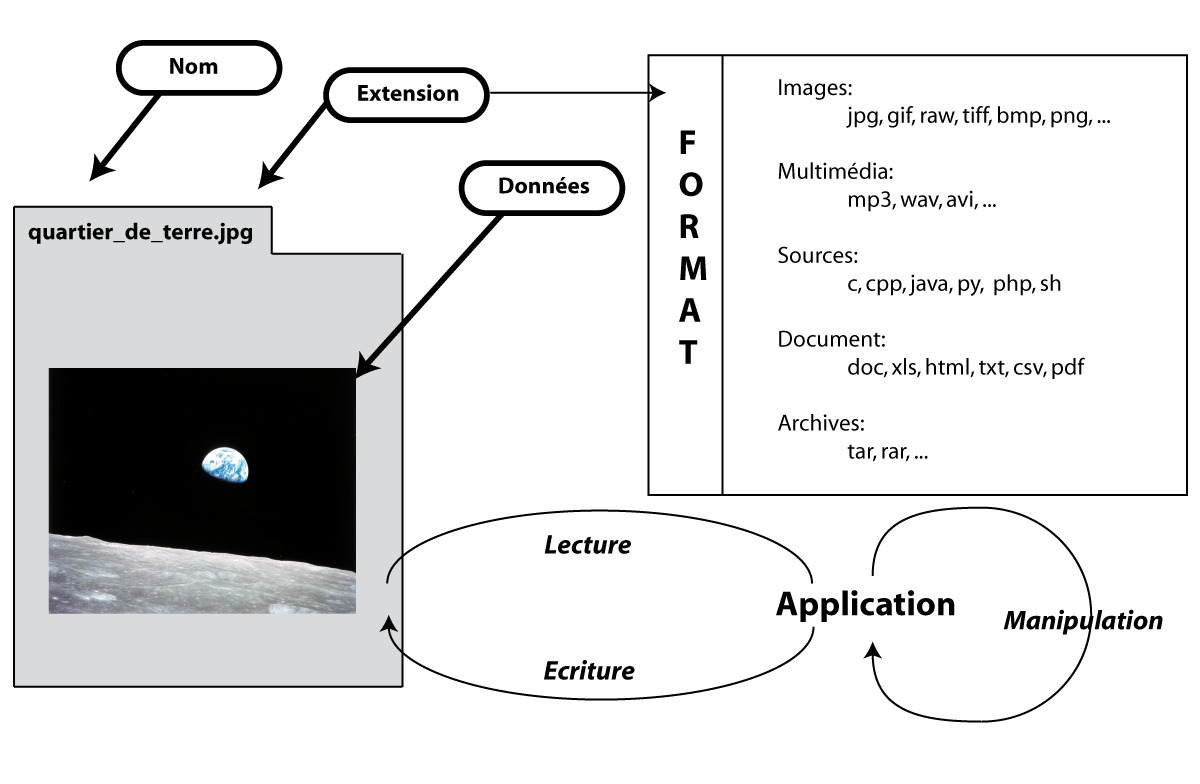
\includegraphics[height=4cm]{img/s03/fichier_1_1.jpg}
    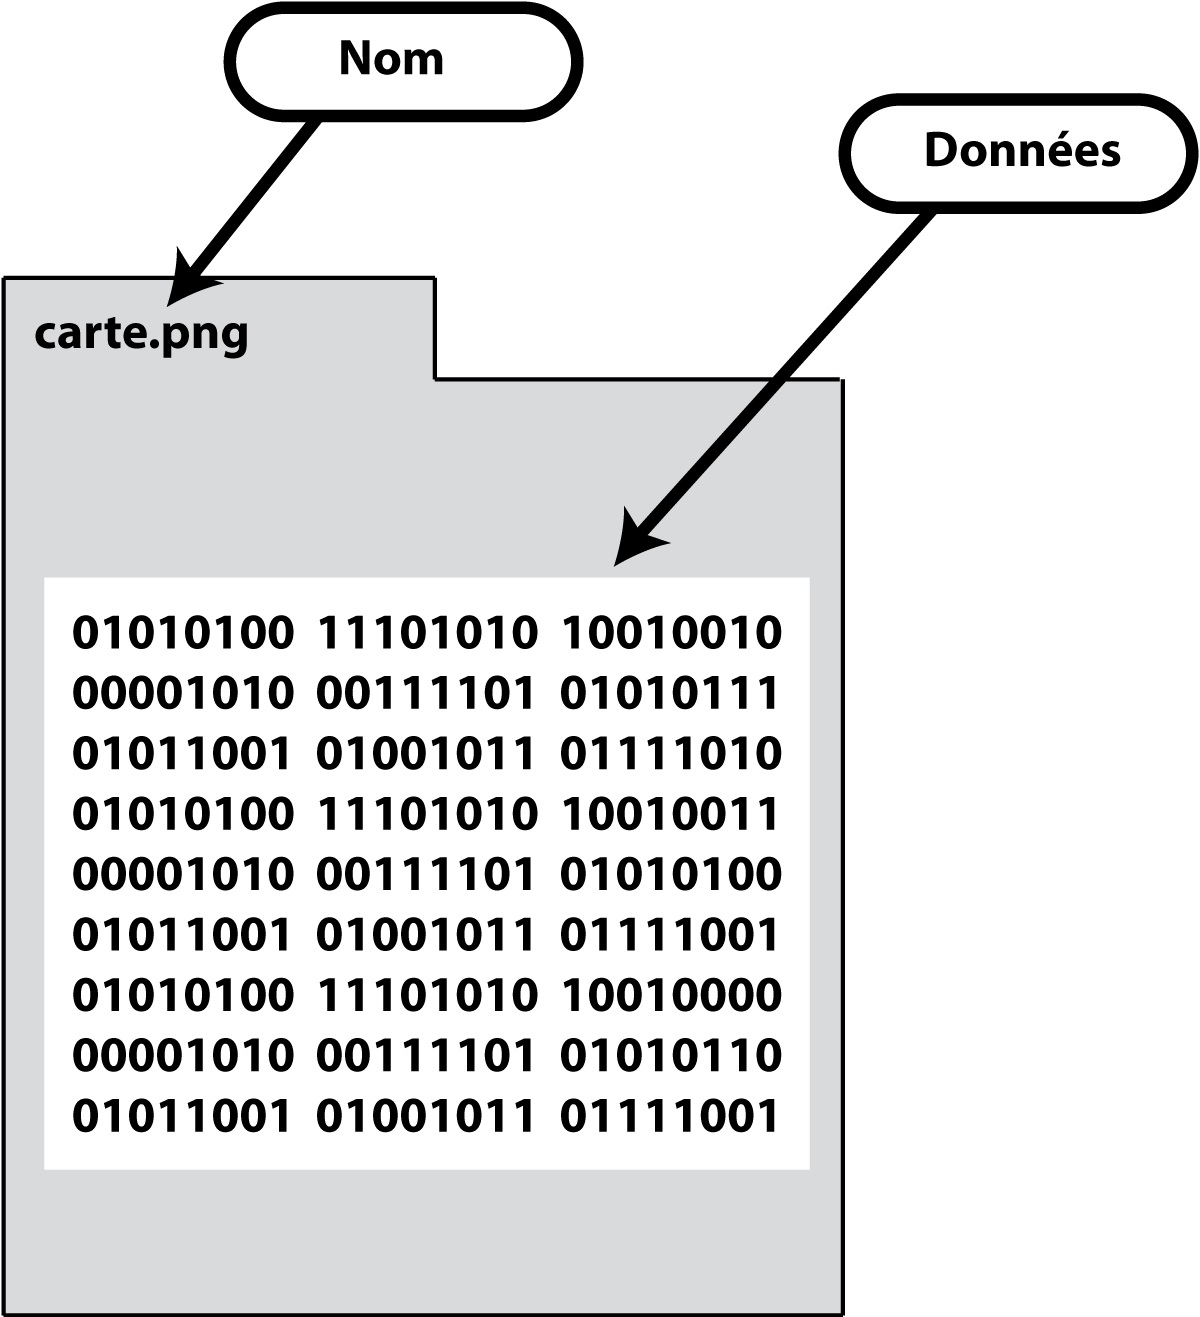
\includegraphics[height=3cm]{img/s03/fichier_1.jpg}
  \end{center}
  \begin{block}{Accès aux données}
    Lors de son utilisation un fichier est \textit{lu} par un
    programme. Pour cela il doit décoder les informations binaires et
    les traiter.
  \end{block}
\end{frame}

\begin{frame}{Fichier binaire et fichier texte}
  \begin{block}{Deux grands types de fichiers: Binaire Vs Numérique}
    De façon générale un fichier binaire ne peut être \textit{"lu"} que
    par un programme informatique, alors qu'un fichier texte peut être
    \textit{"lu"} par être humain.
  \end{block}
  \begin{columns}
    \begin{column}{6cm}
      \begin{block}{Les fichiers textes}
        C'est un fichier qui peut être \textit{"lu"} par un éditeur de
        texte brut. Les données sont encodées comme une suite de
        caractères.
      \end{block}
      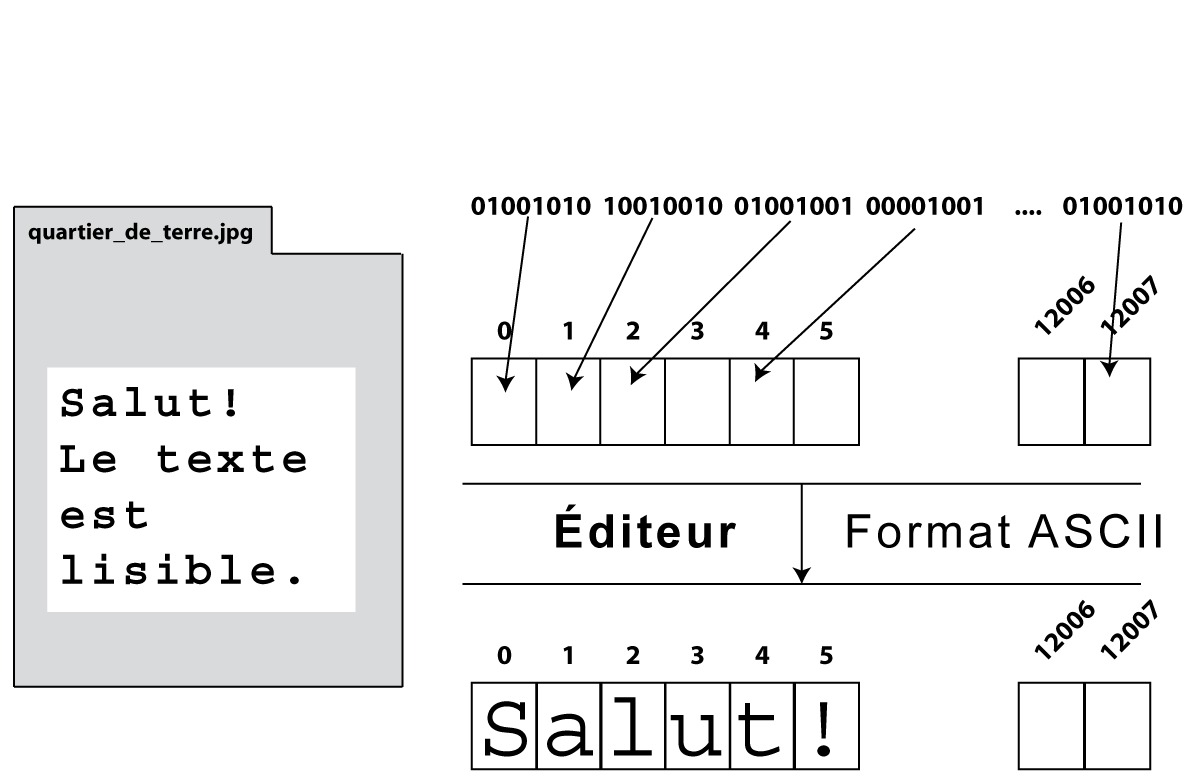
\includegraphics[width=6cm]{img/s03/fichier_1_3.jpg}
    \end{column}
    \begin{column}{6cm}
      \begin{block}{Les fichiers binaires}
        Ce n'est pas un fichier texte \dots Il peut contenir des
        instructions machines, des données compressées, des données
        binaires brutes nécessitant un programme pour être lues.
      \end{block}
      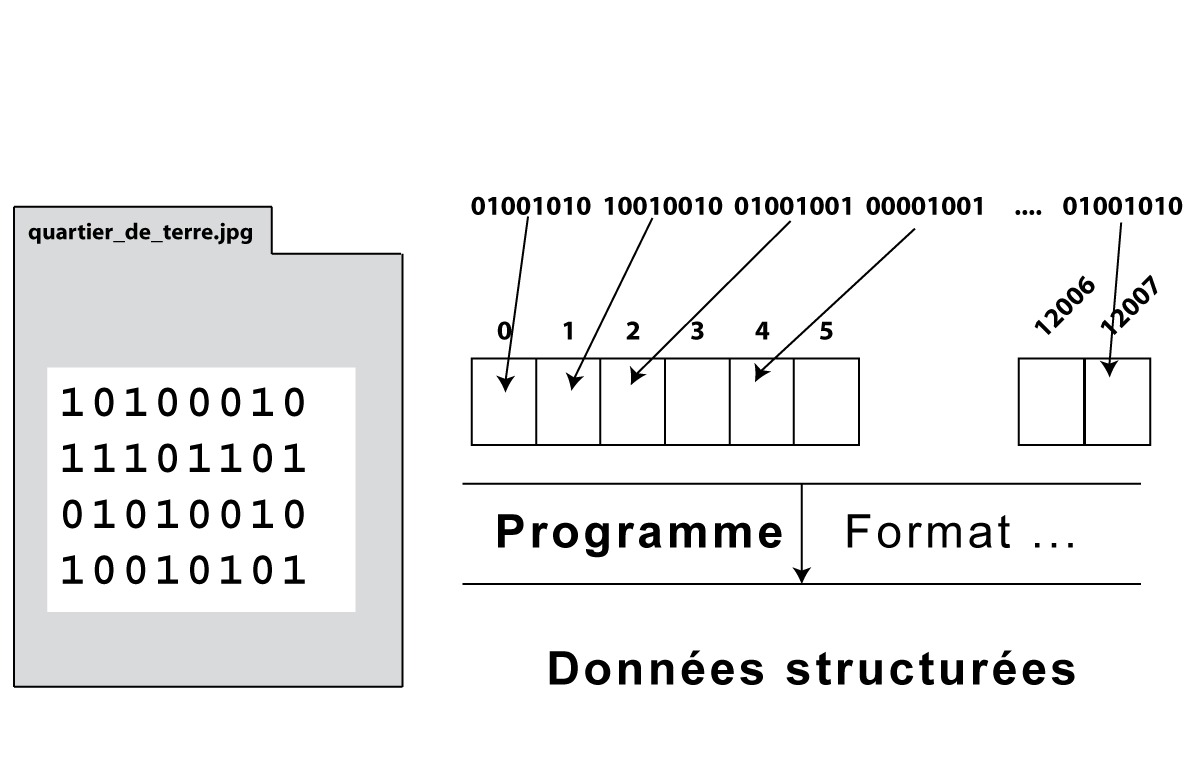
\includegraphics[width=6cm]{img/s03/fichier_1_4.jpg}
    \end{column}
  \end{columns}
\end{frame}
\begin{frame}{Fichiers sources \textrightarrow Exécutable
    \textrightarrow Processus}

  \begin{columns}
    \begin{column}{3.8cm}
      \begin{block}{Les sources: Une \textit{"recette de cuisine"}}
        \begin{itemize}
        \item Exprime un ensemble de tâches à réaliser pour accomplir le
          programme (le plat cuisiné).
        \item Utilise un langage de programmation.
        \item C'est un fichier texte.
        \end{itemize}
      \end{block}
      \fileform[3cm]{dessine.c}{%
        (\dots)\\
        float r, x, y;\\
        r=3.0;\\
        x=0.0;\\
        y=7.1;\\
        cercle(0,0,,r)\\
        segment(0,0,x,y)}
    \end{column}
    \begin{column}{3.8cm}
      \begin{block}{L'exécutable}
        \begin{itemize}
        \item Exprime les mêmes tâches dans un langage machine.
        \item Ce fichier ne fonctionne que sur des ordinateurs qui ont
          la même architecture.
        \item C'est un fichier binaire.
        \end{itemize}
      \end{block}
      \vfill \fileform[3cm]{dessine}{%
        10100101 11101001\\
        10001001 00100101\\
        00101010 00100010\\
        01111011 10110101\\
        01000010 00110011\\
        00101101 11010100\\
        (\dots)}
    \end{column}
    \begin{column}{3.8cm}
      \begin{block}{Les processus}
        \begin{itemize}
        \item L'évaluation des instructions machines engendre des
          processus.
        \item Ces processus sont exécutés par le matériel.
        \item Les instructions machine doivent donc être adaptées au
          matériel.
        \end{itemize}
      \end{block}
      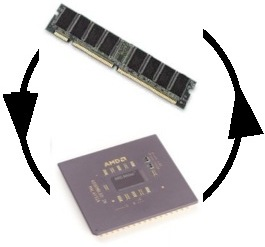
\includegraphics[width=3.5cm]{img/s03/fichier_1_5.jpg}
    \end{column}
  \end{columns}
\end{frame}
\begin{exercice}
  \begin{exercicelet}{Préparation}
    \begin{enumerate}\setcounter{enumi}{\value{cnti}}
    \item Vérifiez que votre répertoire courant est bien
      \verb|TP_2|. Analysez l'affichage produit par la commande ls
      suivie des options \texttt{-lh}. Vous pourrez comparer les
      affichages obtenus par les commandes \texttt{ls -l} et \texttt{ls
        -lh} pour comprendre l'effet de l'option \texttt{-h}. Vous
      pourrez aussi rechercher cette information dans les pages de man.
    \item Analysez l'arborescence créée lors de l'extraction des données
      de l'archive au moyen de la commande \texttt{ls}. Vous dessinerez
      cette arborescence.
    \item Après vous être placé dans le répertoire créé lors de
      l'extraction de l'archive (donnees), quelle commande permet
      d'identifier le plus gros fichier (taille mémoire). Identifiez-le.
    \item Quelles commandes vous permettent d'afficher le contenu des
      fichiers texte \verb|command_line.txt| et \texttt{0readme}? Quels
      sont leurs contenus?
    \item Analysez le résulat de l'évaluation des commandes suivantes:
\begin{verbatim}
 file 0readme
 file commande_line.txt
 file images/solar.png
\end{verbatim}
    \item Quelle est la fonction de la commande \texttt{file}? Parcourez
      les pages de manuel de cette commande.
      \setcounter{cnti}{\value{enumi}}
    \end{enumerate}
  \end{exercicelet}
\end{exercice}

\subsection{Processus dans un système multitâches et mutli-utilisateurs}
\begin{frame}{Identification des processus par le système
    d'exploitation}
  \begin{block}{Système multi-utilisateur}
    \begin{itemize}
    \item Plusieurs utilisateurs partagent les mêmes ressources matériel
      (RAM, CPU, disques, \dots),
    \item Chaque utilisateur lance des processus liés à ses activités
      sur la machine et il utilise les résultats de ces processus.
    \end{itemize}
  \end{block}
  \begin{block}{Système multi-tâches}
    \begin{itemize}
    \item Plusieurs programmes en cours d'exécution partagent les mêmes
      ressources matériel (mémoire vive, CPU, disques, \dots). Ils
      peuvent provenir d'un seul ou de plusieurs utilisateurs,
    \item Chaque programmes lance des processus et il utilise les
      résultats de ces processus.
    \end{itemize}
  \end{block}
  \begin{alertblock}{Il faut partager les ressources !!!}
    \begin{itemize}
    \item Chaque programme doit être exécuté éventuellement \textit{"en
        même temps"}. Il faut donc gérer le partage des ressources de
      calcul (accès à la mémoire vive, au CPU),
    \item Chaque programme ou utilisateur doit pouvoir retrouver les
      résultats de ses calculs. Il faut donc pouvoir identifier qui a
      lancé les processus et qui doit récupérer les résultats.
    \end{itemize}
    La gestion des processus est réalisée par le système
    d'exploitation. C'est une de ses tâches principales. Pour cela il a
    besoin de pouvoir identifier chaque processus.
  \end{alertblock}
\end{frame}
\begin{frame}{PID et PPID}
  \begin{block}{PID - \textbf{P}rocess \textbf{ID}entifier}
    \begin{itemize}
    \item C'est un numéro unique attribué à chaque processus lors de son
      lancement.
    \item Il permet d'identifier de façon unique chaque processus.
    \item La liste des processus en cours d'exécution est accessible en
      ligne de commande par les commandes \lin{ps} et \lin{top}.
    \end{itemize}
  \end{block}
  \begin{block}{PPID - \textbf{P}arent \textbf{P}rocess
      \textbf{ID}entifier}
    \begin{itemize}
    \item Le premier processus lancé porte le numéro de PID 1. Les
      processus suivants sont des processus issus de ce processus
      parent.
    \item Chaque processus est lancé par un processus parent
      \textit{via} l'appel système \lin{fork}.
    \item Le PPID est le PID du processus Parent.
    \end{itemize}
  \end{block}
  \begin{block}{Utilités}
    \begin{itemize}
    \item L'utilisateur peut suivre un processus, le suspendre
      temporairement, le relancer ou le tuer (interruption définitive).
    \item Le système s'en sert pour lui affecter des ressources
      matériel.
    \end{itemize}
  \end{block}
\end{frame}

\begin{exercice}
  \begin{exercicelet}{Racourcis clavier et astuces en ligne de commande}
    \begin{enumerate}\setcounter{enumi}{\value{cnti}}
      \setcounter{cnti}{\value{enumi}}
    \item Tapez les 2 caractères \texttt{sl} puis pressez la touche \Tab
      (Tab). Que se passe-t-il?
    \item Tapez les 3 caractères \texttt{sle} puis pressez la touche
      \Tab. Que se passe-t-il?
    \item À la suite de l'affichage précédent tapez la combinaison de
      touches \Ctrl\keystroke{A}. Que se passe-t-il?
    \item Que fait la commande \texttt{man sleep}? Que pouvez-vous dire
      de la commande \texttt{sleep}?
    \item Exécutez la commande \texttt{sleep 32000000}. Que se
      passe-t-il si vous tapez la combinaison de touches
      \Ctrl\keystroke{C}?
    \item Quelle action produit la pression de la flèche \UArrow sur
      votre clavier?
    \item Quelle est l'action produite par la pression de la combinaison
      de touches \Ctrl\keystroke{U} après avoir tapé quelques lettres?
      Par la combinaison de touche \Ctrl\keystroke{L}?
    \item Quelle est l'action produite en tapant ls\Spacebar\Tab (le
      caractère \Spacebar signifie la présence d'un espace)?
    \end{enumerate}
  \end{exercicelet}
\end{exercice}

\subsection{Gestion de la mémoire vive}
\begin{frame}{Gestion de la mémoire vive}
  \begin{columns}
    \begin{column}{6cm}
      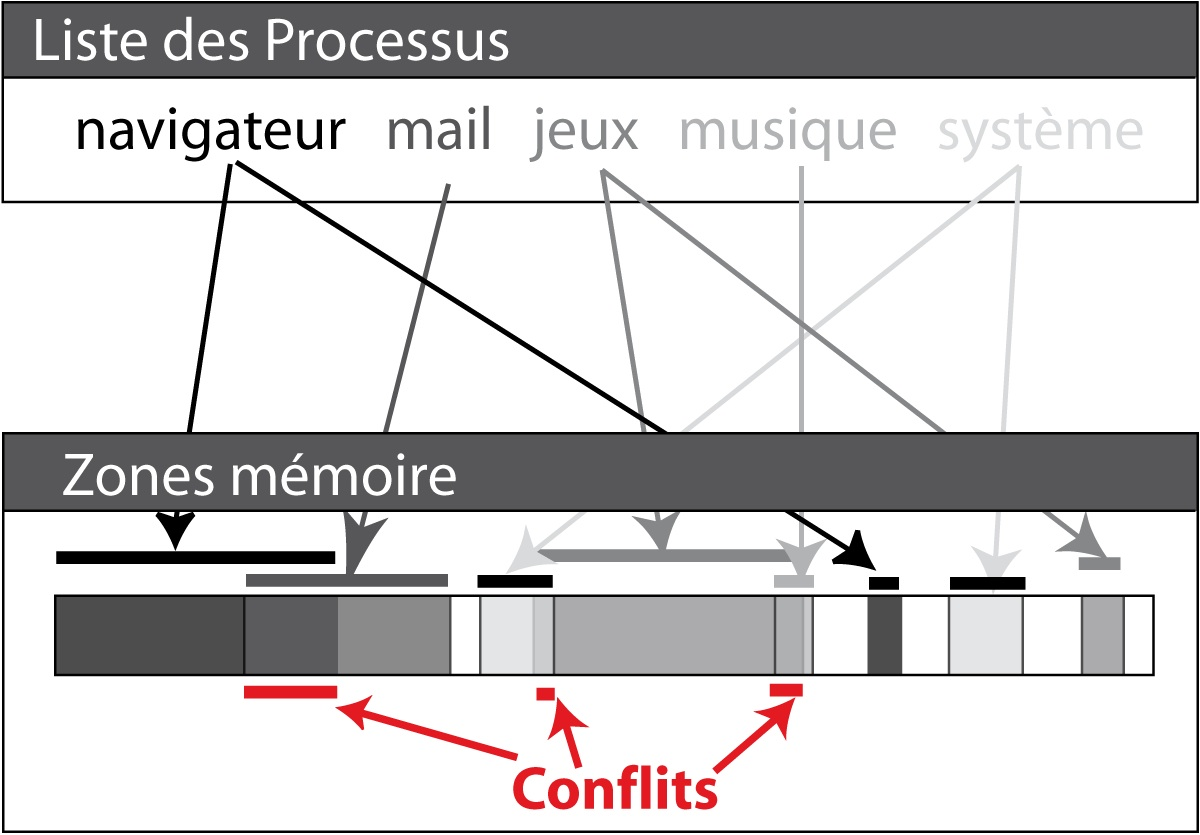
\includegraphics[width=5.5cm]{img/s03/Alloc_mem_1.jpg}
      \begin{block}{Chaque processus a besoin de mémoire}
        Pour stocker et travailler sur:
        \begin{itemize}
        \item les données,
        \item les instructions,
        \item les résultats.
        \end{itemize}
      \end{block}
      \begin{alertblock}{Il faut assurer l'intégrité des données !}
      \end{alertblock}
    \end{column}
    \begin{column}{6cm}
      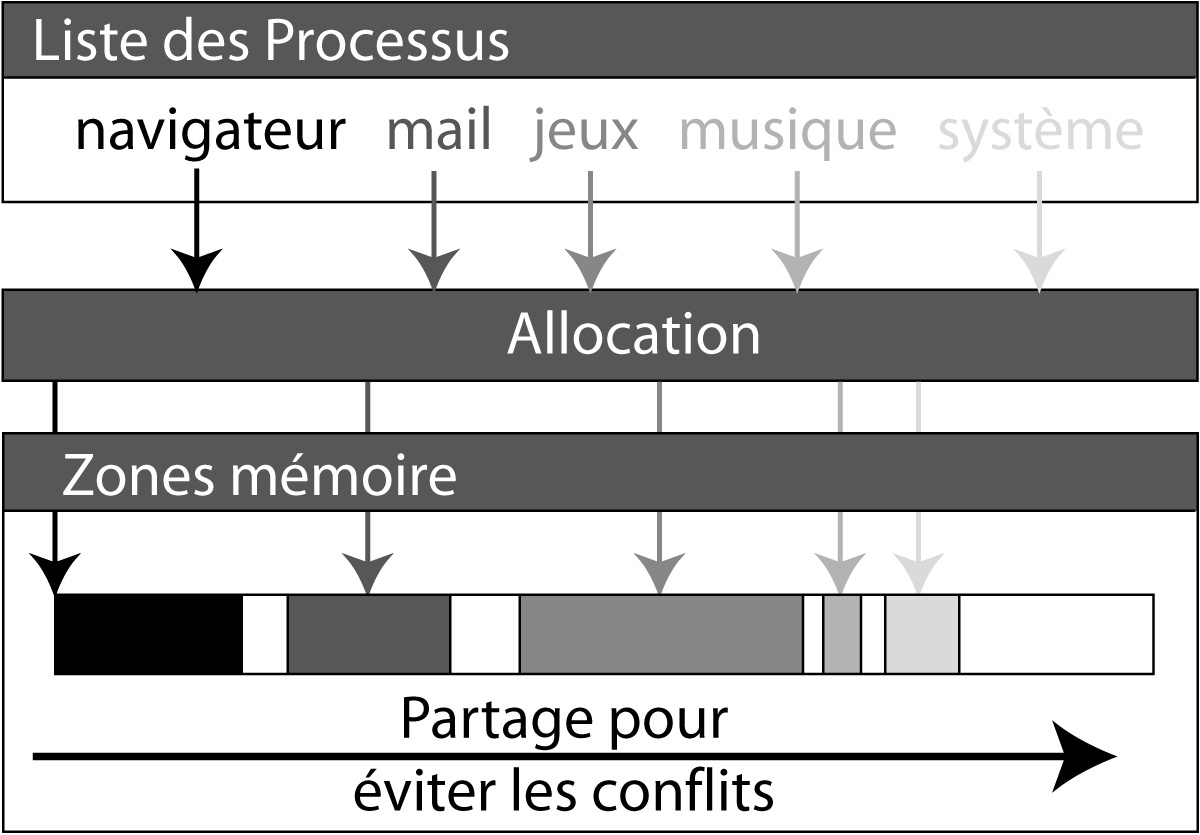
\includegraphics[width=5.5cm]{img/s03/Alloc_mem_2.jpg}
      \begin{block}{Allocation de zone mémoire}
        L'allocation permet:
        \begin{itemize}
        \item d'attribuer à chaque processus un espace de travail en
          mémoire,
        \item le système contraint le programme à écrire dans sa zone
          mémoire et ainsi,
        \item évite qu'un programme modifie les données d'un autre
          programme.
        \end{itemize}
      \end{block}
    \end{column}
  \end{columns}
\end{frame}
\begin{frame}{Gestion de la mémoire vive}
  \begin{center}
    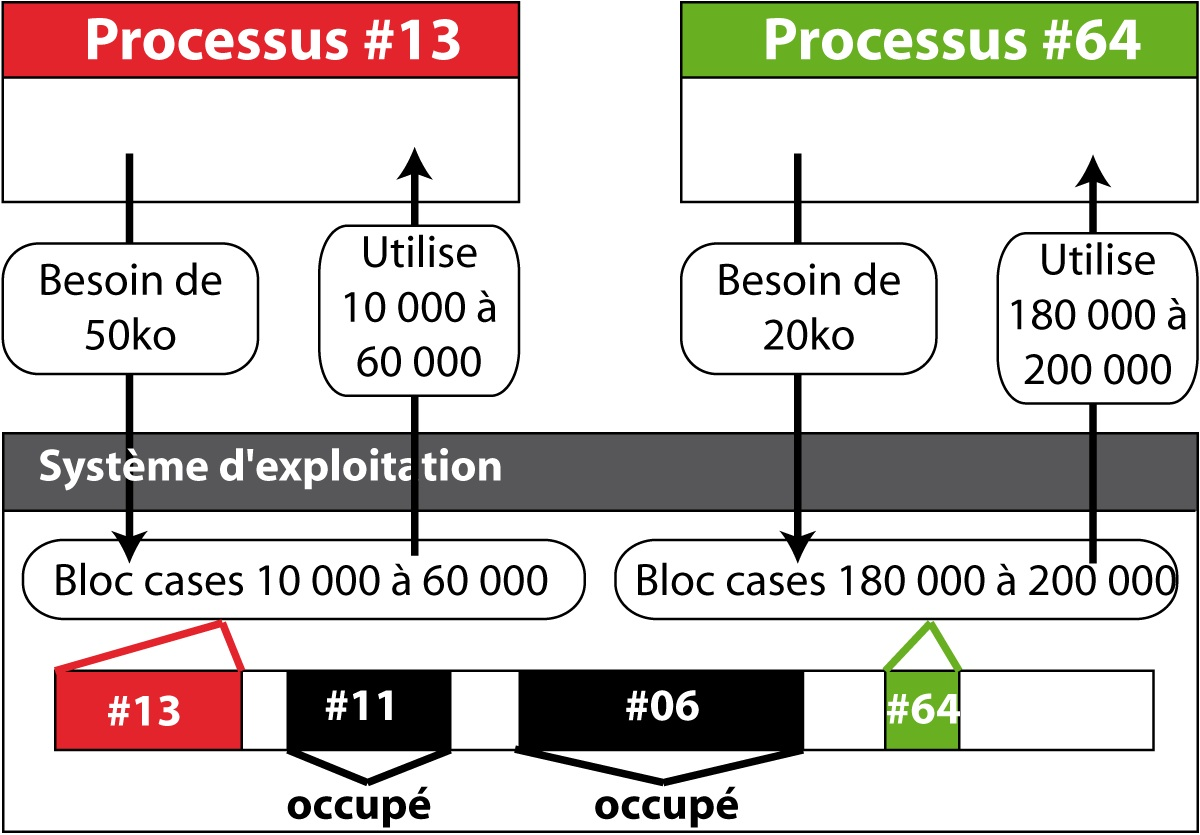
\includegraphics[width=7cm]{img/s03/Alloc_mem_3.jpg}
  \end{center}
  \begin{block}{Principes généraux de l'allocation}
    \begin{itemize}
    \item L'OS maintient une table des zones mémoires allouées à chaque
      processus. Ces zones sont réservées et ne peuvent être utilisées
      que par le processus parent.
    \item Lorsqu'il a besoin de mémoire, un processus demande à l'OS
      quelle zone il peut utiliser,
    \item L'OS lui attribue, en fonction de l'espace libre, un certain
      nombre de blocs mémoire.
    \item Les blocs mémoire attribués sont alors réservés.
    \end{itemize}
  \end{block}
\end{frame}
\subsection{Gestion de l'accès au CPU}
\begin{frame}{Gestion de l'accès au CPU}
  \begin{center}
    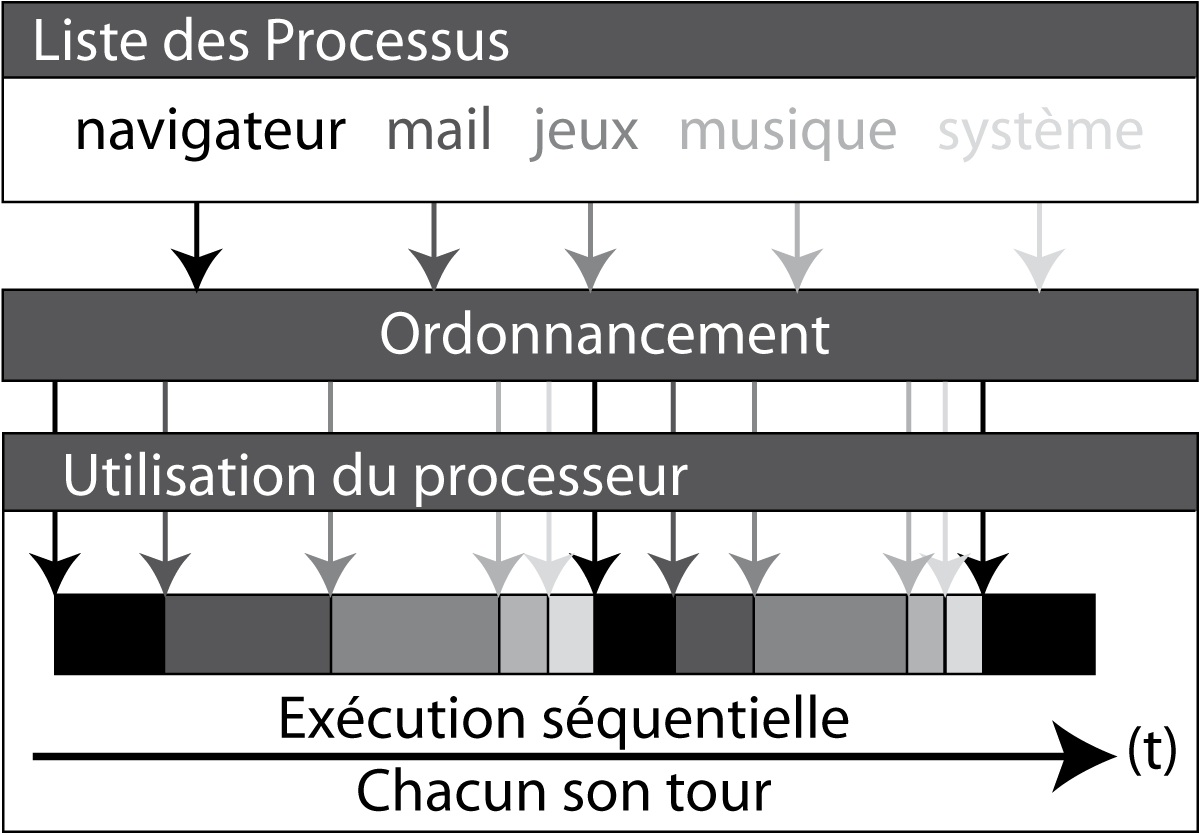
\includegraphics[width=7cm]{img/s03/Planificateur.jpg}
  \end{center}
  \begin{block}{Le planificateur gère le temps CPU attribué à chaque
      processus}
    \begin{itemize}
    \item Le CPU ne traite qu'un seul processus à la fois,
    \item Le planificateur permet l'alternance d'accès au CPU en
      attribuant une priorité à chaque processus.
    \item L'illusion d'exécution simultanée de plusieurs processus est
      donnée par une alternance rapide d'attribution de temps de calcul
      à chaque processus.
    \end{itemize}
  \end{block}
\end{frame}

\manpage{ps} \manpage{top}

\subsection{Processus en ligne de commande}
\begin{frame}{Processus en ligne de commande}
  \begin{block}{Occupation de la ligne de commande}
    \begin{itemize}
    \item Lorsque l'on tape une commande, la ligne de commande est
      bloquée (plus de prompt) jusqu'à la fin de l'exécution.
    \item La ligne de commande est à nouveau disponible ensuite.
    \end{itemize}
    \begin{center}
      \mprompt{ \prompt{sleep 20}{{\color{solarizedBlue}(\textit{il faut
              attendre 20 secondes avant l'apparition du nouveau
              prompt)\\\dots\\\dots}}} \prompt{\cursor}{} } \mprompt{
        \prompt{gedit}{{\color{solarizedBlue}(\textit{Il faut quitter
              l'application ou tuer le processus \lin{gedit} pour avoir
              un nouveau prompt)\\\dots\\\dots}}} }
    \end{center}
  \end{block}
\end{frame}

\begin{frame}{Libération de la ligne de commande}
  Deux façons possibles de lancer une instruction en tâche de fond:
  \begin{columns}
    \begin{column}{6cm}
      \begin{block}{Lancement en tâche de fond}
        \begin{itemize}
        \item Les commandes qui prennent beaucoup de temps peuvent être
          lancées en tâche de fond pour libérer la ligne de commande du
          shell.
        \item Pour lancer directement la commande en tâche de fond il
          suffit de faire suivre la commande du caractère
          {\color{red}\lin{\&}}. On retrouve immédiatement un nouveau
          prompt.
        \end{itemize}
        \vspace{20pt}
        \begin{center}
          \scriptsize{ \mpromptS{ \promptS{gedit \&}{}
              \promptS{\cursor}{} } }
        \end{center}
      \end{block}
    \end{column}
    \begin{column}{6cm}
      \begin{block}{Relégation en tâche de fond}
        \begin{itemize}
        \item Si une tâche déjà lancée occupe la ligne de commande, il
          est possible de suspendre son exécution en pressant la
          combinaison de touches \Ctrl\keystroke{Z}. La tâche est alors
          interrompue et on retrouve un nouveau prompt.
        \item Il est possible de relancer le processus en tâche de fond
          au moyen de la commande \lin{bg}.
        \end{itemize}
        \begin{center}
          \scriptsize{ \mpromptS{
              \promptS{gedit}{\^{}Z\\\string[1\string]\string$+ Stopped
                gedit} \promptS{bg}{\string[1\string]\string$+ gedit \&}
              \promptS{\cursor}{} } }
        \end{center}
      \end{block}
    \end{column}
  \end{columns}
\end{frame}

\begin{exercice}
  \begin{exercicelet}{Gestion des processus}
    Afin d'illustrer la gestion des processus nous allons utiliser la
    commande \texttt{sleep} pour simuler l'exécution de programmes dont
    l'exécution n'est pas immédiate. Pour se rappeler de son
    fonctionnement vous pouvez utiliser la commande man.
    \begin{enumerate}\setcounter{enumi}{\value{cnti}}
    \item Évaluez l'instruction \verb|sleep 1000| puis tapez
      \Ctrl\keystroke{C}. Que se passe-t-il?
    \item Évaluez l'instruction \verb|sleep 1000 &| (n'oubliez pas le
      caractère \verb|&|). Que se passe-t-il?
    \item La commande ps permet d'afficher la liste de processus qui
      s'exécutent sur votre ordinateur. Un processus s'exécutant sous
      Linux est identifié par un numéro de processus, et par un
      propriétaire (celui qui a lancé le processus). Identifiez ces deux
      données lors de l'appel des commandes suivantes, donnez un
      explication à la différence des affichages (utilisez le man si
      nécessaire):
\begin{verbatim}
ps
ps -ef
\end{verbatim}
    \item Quel est le numéro de processus associé à la commande
      \verb|sleep 1000 &|?
      \setcounter{cnti}{\value{enumi}}
    \end{enumerate}
  \end{exercicelet}
\end{exercice}
\begin{exercice}
  \begin{exercicelet}{Gestion des processus (suite)}
    \begin{enumerate}\setcounter{enumi}{\value{cnti}}
      \setcounter{cnti}{\value{enumi}}
    \item La commande kill permet de «~tuer~» (supprimer) un
      processus. Sa syntaxe d'utilisation est la suivante: \texttt{kill
        PID} où PID (Process ID) doit être remplacé par le numéro du
      processus à supprimer.  \setcounter{cnti}{\value{enumi}}
    \item Quelle commande permet de détruire le processus associé à
      la commande \verb|sleep 1000 &|?
    \item Tapez la commande \texttt{gedit} dans le terminal. Quel
      est l'effet sur la ligne de commande? Pouvez-vous saisir de
      nouvelle commandes?
    \item Après avoir lancé \texttt{gedit} (celui-ci étant en cours
      d'exécution), que se passe-t-il si on tape \Ctrl\keystroke{Z} dans
      le terminal qui a lancé \texttt{gedit}? Quel est l'effet sur le programme
      gedit (utilisez \texttt{ps} pour suivre l'état des processus)? Que se
      passe-t-il si vous tapez \texttt{bg}?
    \item Que fait la commande \texttt{top}?
    \item Exécutez la command \texttt{ps -ef f}. Examinez comment est
      construite la \emph{forêt} de processus. Repérez comment sont
      agencés les processus qui gèrent vos terminaux entre eux.
      \setcounter{cnti}{\value{enumi}}
    \end{enumerate}
  \end{exercicelet}
\end{exercice}

\section{Compléments sur l'arborescence}
\subsection{Droits sur les fichiers}
\begin{frame}{Propriété des fichiers}
  \begin{block}{Identifications des utilisateurs dans un environnement
      multi-utilisateurs}
    \begin{enumerate}
    \item[UID] (\textbf{U}ser \textbf{ID}entifier) numéro unique associé à
      chaque utilisateur lors de la création de son compte.
    \item[GID] (\textbf{G}roup \textbf{ID}entifier) numéro unique d'un groupe
      d'utilisateurs. Chaque utilisateur peut être associé à un ou plusieurs
      groupes.
    \end{enumerate}
  \end{block}
  \begin{alertblock}{Utilité}
    \begin{itemize}
    \item Chaque fichier (ou répertoire) et chaque processus du système est
      associé à un utilisateur: cet utilisateur est le propriétaire du fichier
      (ou répertoire) ou celui qui a lancé le processus.
    \item Être propriétaire d'un fichier ou d'un processus confère des droits
      sur ceux-ci.
    \end{itemize}
  \end{alertblock}
  \begin{block}{Connaitre l'identité du propriétaire d'un processus ou d'un
      fichier}
    \begin{itemize}
    \item Les commandes \lin{top} et \lin{ps} affichent le nom du propriétaire
      des processus.
    \item La commande \lin{ls} avec l'option \lin{-l} affiche le nom et le
      groupe du propriétaire d'un fichier ou d'un répertoire.
    \item Les UID et GID sont enregistrés dans le fichier d'administration
      \lin{/etc/passwd} ou d'autres mécanismes
    \end{itemize}
  \end{block}
\end{frame}

\manpage{ls(ter)}
\begin{frame}{Les droits sur les fichiers et répertoires}
  \begin{block}{3 catégories d'utilisateurs}
    \begin{center}
      \begin{tabular}{c|ccc|ccc|ccc}
        \Huge{-}&\Huge{r}&\Huge{w}&\Huge{x}&\Huge{r}&\Huge{w}&\Huge{x}&\Huge{r}&\Huge{w}&\Huge{x}\\
        &&&&&&&&&\\
        Type de&\multicolumn{3}{c|}{Doits du}&\multicolumn{3}{c|}{Doits du}&\multicolumn{3}{c}{Doits des}\\
        Fichier&\multicolumn{3}{c|}{propriétaire}&\multicolumn{3}{c|}{groupe}&\multicolumn{3}{c}{autres}\\
        &\multicolumn{3}{c|}{(\textbf{U}ser)}&\multicolumn{3}{c|}{(\textbf{G}roup)}&\multicolumn{3}{c}{(\textbf{O}ther)}\\
      \end{tabular}
    \end{center}
  \end{block}
  \begin{columns}
    \begin{column}{3.5cm}
      \begin{block}{Types de fichiers}
        \begin{center}
          \begin{tabular}{ll}
            \hline
            &Types\\
            \hline
            -&Fichier ordinaire\\
            d&Répertoire\\
            l&lien symbolique\\
            \hline
          \end{tabular}
        \end{center}
      \end{block}
    \end{column}
    \begin{column}{8cm}
      \begin{block}{Droits/Permissions}
        \begin{center}
          \begin{tabular}{llll}
            \hline
            &&Fichier&Répertoire\\
            \hline
            \lin{r}&(\textbf{R}ead)&lire&lister le contenu\\
            \lin{w}&(\textbf{W}rite)&écrire et modifier&modifier le contenu\\
            \lin{x}&(e\textbf{X}ecute)&exécution&traverser\\
            \hline
          \end{tabular}
        \end{center}
      \end{block}
    \end{column}
  \end{columns}
  \begin{block}{Types d'utilisateurs}
    \begin{center}
      \begin{tabular}{lll}
        \hline
        && Cible\\
        \hline
        u&(\textbf{U})ser&Propriétaire du fichier/répertoire\\
        g&(\textbf{G})roup&Membre du même groupe que le propriétaire\\
        o&(\textbf{O})ther&Tous les autres\\
        a&(\textbf{A})ll&Tous les utilisateurs (réunion de \lin{'u'}, \lin{'g'} et \lin{'o'}).\\
        \hline
      \end{tabular}
    \end{center}
  \end{block}
\end{frame}

\manpage{chmod} \manpage{chmod(bis)}

\begin{exercice}
  \begin{exercicelet}{Identification et droits}
    \begin{questions}
    \item Au moyen de la commande \lin{id}, affichez votre UID et votre GID?
      Comparez-le avec celui de votre voisin de table. Qu'en concluez-vous?
      Comparez-les avec celui de l'utilisateur \lin{root}. Qu'en
      concluez-vous?
    \item Quels sont vos droits sur le répertoire racine \lin{/}, \lin{root},
      \lin{/tmp}, sur votre répertoire \lin{\~\//}, et celui de votre voisin
      de table \lin{\~\//../login\_voisin}.
    \item Pouvez-vous lire les données contenue dans le répertoire de votre
      voisin. Quelle commande permettrait de le faire? Qui doit lancer la
      commande?
    \item Donnez les commandes octale et alphanumérique de changement de
      droits permettant:
      \begin{itemize}
      \item d'autoriser aux membres de votre groupe et aux "autres" l'accès en
        lecture aux images du répertoire \lin{donnees\_tdtp2/images}.
      \item de donnez les droits d'écriture aux membres de votre groupe sur le
        fichier \lin{donnees\_tdtp2/command\_line.txt}
      \item de vous (le propriétaire) retirer toute possibilité de supprimer
        le fichier \lin{donnees\_tdtp2/0readme}
      \end{itemize}
    \item Imaginez comment donner à votre voisin un accès sous votre
      répertoire personnel à un répertoire dans lequel il aurait les droits
      d'écriture sur un fichier spécifique, que vous ne pourriez vous que lire
      (mais pas modifier). Il ne doit pas pouvoir créer un autre fichier chez
      vous. Comment faites vous pour effacer ce fichier ?
    \end{questions}
  \end{exercicelet}
\end{exercice}
\begin{exercice}
  \begin{exercicelet}{Remise en état}
    Après toutes les modifications pouvant impliquer votre répertoire
    personnel, n'oubliez pas \lin{chmod 711 ~} pour remettre les modes de
    votre répertoire à leur état d'origine.
  \end{exercicelet}
\end{exercice}
\subsection{Arborescence du système Linux}
\begin{frame}{Les principaux répertoires et leur contenu}
  \begin{block}{Une structure plus ou moins normalisée}
    \begin{itemize}
    \item Les fichiers nécessaires au fonctionnement du système sont organisés
      en arborescence,
    \item Cette arborescence est commune à presque toutes les distribution
      linux,
    \item Cette organisation rationalisée facilite l'installation de nouveaux
      programmes qui savent où trouver les fichiers dont ils peuvent avoir
      besoin.
    \end{itemize}
  \end{block}
  \begin{block}{Une organisation qui permet un cloisonnement}
    \begin{itemize}
    \item Les fichiers et les répertoires systèmes sont protégés par des
      restrictions de droits,
    \item De nombreux fichiers ne peuvent être modifiés par un utilisateur
      «~normal~»,
    \item Seul l'utilisateur \lin{root}, ou les utilisateur faisant partie du
      groupe \lin{admin} peuvent avoir la permission de modifier certains
      fichiers.
    \item Il s'agit d'une protection. Pour réaliser une action susceptible
      d'affecter le comportement du système il faut montrer "patte blanche" et
      prendre conscience de ce que l'on fait. Entrer le mot de passe
      \lin{root} doit être un signal d'alerte.
    \end{itemize}
  \end{block}
\end{frame}

\begin{frame}{Les principaux répertoires et leur contenu}
  \begin{center}
    \begin{tabular}{ll}
      \hline
      Répertoire&Contenu\\[3pt]
      \hline
      /		&Répertoire racine: Toutes les données accessibles par le système\\[3pt]
      /bin		&Binaires exécutables des commandes de bases (cd, ls, mkdir, \dots)\\[3pt]
      /dev		&Fichiers spéciaux correspondants aux périphériques\\[3pt]
      /etc		&Fichiers de configuration (profile, passwd,fstab... )\\[3pt]
      /home	&Les répertoires personnels des utilisateurs\\[3pt]
      /lib		&Librairies partagées et modules du noyeau\\[3pt]
      /mnt		&Points de montage des périphériques\\[3pt]
      /root		&Répertoire personnel de l'administrateur\\[3pt]
      /tmp		&Données temporaires\\[3pt]
      /usr		&Ressources accessibles par les utilisateurs\\[3pt]
      /var		&Fichiers de log ou fichiers changeant fréquemment\\[3pt]
      \hline
    \end{tabular}
  \end{center}
  L'essentiel est synthétisé dans
  \url{https://fr.wikipedia.org/wiki/Filesystem_Hierarchy_Standard}
\end{frame}
\begin{exercice}
  \begin{exercicelet}{Hiérarchie du système}
    \begin{itemize}
    \item[\ddialoginformation] Astuce: si la sortie d'une commande est trop
      longue, on peut ajouter \verb/|less/ à la fin de la ligne pour
      l'afficher par morceaux. Ceci vous sera expliqué dans quelques
      séances...
    \end{itemize}
    \begin{questions}
    \item Identifiez le propriétaire, le groupe et les différents droits des
      fichiers contenus dans le répertoire \lin{/bin}? Quels sont vos droits
      sur ces fichiers?
    \item Ces fichiers on le droit \lin{x}. Que pouvez-vous en conclure?
    \item A votre avis, que se passe-t-il en fait lorsque vous saisissez une
      commande telle que \lin{ls} ?
    \end{questions}
  \end{exercicelet}
  \begin{exercicelet}{FHS}
    \begin{questions}
    \item Identifiez, à l'aide de la FHS, la fonction de
      \lin{/usr/include}. Confirmez votre hypothèse en regardant quelques
      fichiers.
    \end{questions}
  \end{exercicelet}
\end{exercice}

\subsection{Interprétation ou Compilation}
\begin{frame}{Langages Compilés Vs Langages Interprétés}
  \begin{block}{Caractéristiques des Langages
      \only<1|handout:1>{Compilés}\only<2|handout:2>{Interprétes}}
    \only<1|handout:1>{%
      \begin{itemize}
      \item L'ensemble du code source est compilé une seule fois avant
        l'exécution en instructions machine (contenues dans un fichier:
        exécutable).
      \item Le compilateur n'est pas nécessaire lors de l'exécution.
      \item Le compilateur est spécifique à la machine.
      \item L'exécutable (code compilé) est spécifique à la machine.
      \end{itemize}
    } \only<2|handout:2>{%
      \begin{itemize}
      \item Les instructions du code source sont converties en instructions
        machine lors de l'exécution du programme
      \item L'interpréteur est nécessaire lors de l'exécution.
      \item L'interpréteur est spécifique à la machine,
      \item L'exécutable (le code source) n'est pas spécifique à la machine.
      \end{itemize}
    }
  \end{block}
  \begin{columns}
    \begin{column}{5.5cm}
      \begin{block}{Inconvenients}
        \only<1|handout:1>{%
          \begin{itemize}
          \item Il faut recompiler pour prendre en compte une modification du
            code.
          \item L'exécutable n'est pas portable sur d'autres machines.
          \end{itemize}
        } \only<2|handout:2>{%
          \begin{itemize}
          \item Moins rapide.
          \item Plusieurs fichiers (et librairies) servent à l'exécution.
          \end{itemize}
        }
      \end{block}
    \end{column}
    \begin{column}{5.5cm}
      \begin{block}{Avantages}
        \only<1|handout:1>{%
          \begin{itemize}
          \item Plus rapide (spécifique à la machine qui exécute les
            instructions).
          \item L'ensemble des instructions sont regroupées dans un seul
            fichier.
          \end{itemize}
        } \only<2|handout:2>{%
          \begin{itemize}
          \item Modifications du code source immédiatement prises en compte
            lors de la réexécution.
          \item Le code est portable sur d'autres machine
          \end{itemize}
        }
      \end{block}
    \end{column}
  \end{columns}
  \begin{block}{Exemples de langages \only<1>{Compilés}\only<2>{Interprétés}}
    \only<1|handout:1>{%
      \begin{itemize}
      \item C, C++, ADA, Pascal, Fortran, Cobol,
      \end{itemize}
    } \only<2|handout:2>{%
      \begin{itemize}
      \item Java, Python, Bash, Lisp, PHP, Prolog, Perl, Javascript
      \end{itemize}
    }
  \end{block}
\end{frame}

\subsection{Exécution des commandes}
\begin{frame}{Lancer un programme/une commande}
  \begin{block}{Cas général}
    \begin{itemize}
    \item Pour exécuter un programme il suffit saisir sur la ligne de commande
      le chemin menant au fichier contenant les instructions,
    \item Si le fichier présente la permission \lin{"X"} pour exécutable, les
      instructions qu'il contient sont exécutées.
    \end{itemize}
  \end{block}
  \begin{columns}
    \begin{column}{.45\textwidth}
      \begin{block}{Script {bash} exécutable}
        \begin{itemize}
        \item Un script \lin{bash} est un fichier texte contenant des
          instructions \lin{bash}
        \item La première ligne contient le chemin menant à l'exécutable de
          l'interpréter précédé des caractère \lin{\#!} (par exemple \lin{\#!
            /bin/bash}),
        \item La seconde ligne est souvent vide,
        \item Les lignes suivantes comportent des instructions.
        \end{itemize}
      \end{block}
    \end{column}
    \begin{column}{.45\textwidth}
      
      \fileform[.8\textwidth]{test\_bash.sh}{%
        \#!/bin/bash\\ \\instruction 1 ;\\instruction 2 ;\\...\\instruction N
        ; }
    \end{column}
  \end{columns}
\end{frame}

\begin{exercice}
  \begin{exercicelet}{Lancer un programme/une commande}
    \begin{questions}
    \item Après avoir créé un répertoire \lin{bin} dans votre répertoire
      personnel, définissez créez dans ce répertoire un script nommé
      \lin{listintro.sh}. Ce script comporte une unique commande permettant de
      lister le contenu du répertoire de travail
      \lin{Intro\_Systeme} dans lequel vous avez l'habitude de travailler.
    \item Attribuez les droits d'exécution sur ce fichier. Il est normalement
      devenu un exécutable.
    \item Quelle commande permet d'exécuter ce script si le répertoire courant
      es le répertoire \lin{\~\//bin} qui le contient? Idem, si le répertoire
      courant est votre répertoire personnel. Vous vérifierez que le script se
      comporte comme attendu (il vous place dans une autre répertoire).
    \item la commande \lin{echo} permet d'afficher une message à
      l'écran. Modifiez le script pour qu'il avertisse l'utilisateur du
      changement de répertoire par un message explicite.
    \end{questions}
  \end{exercicelet}
\end{exercice}

\manpage{echo}

\begin{frame}{Lancer un programme/une commande}
  \begin{block}{Cas général}
    \begin{itemize}
    \item Pour exécuter un programme il suffit saisir sur la ligne de commande
      le chemin menant au fichier contenant les instructions,
    \item Si le fichier présente la permission \lin{"X"} pour exécutable, les
      instructions qu'il contient sont exécutées.
    \end{itemize}
  \end{block}
  \begin{block}{Cas particulier : les commandes}
    \begin{itemize}
    \item Une commande (\lin{ls}, \lin{gedit}, \lin{firefox}, \dots) est un
      programme comme un autre,
    \item Les instructions qui doivent être évaluées sont écrites dans un
      fichier (\lin{/bin/ls}, \lin{/usr/bin/python},
      \lin{/usr/share/bin/firefox}, \dots),
    \item Pourtant \dots
    \end{itemize}
  \end{block}
  \begin{alertblock}{Des chemins qui mènent nulle part !!!}
    \begin{itemize}
    \item les noms des commandes (\lin{ls}, \lin{gedit}, \lin{firefox} \dots)
      sont toujours saisies comme des chemins relatifs (pas de \lin{/bin/...}
      devant le nom du fichier), alors que le fichier de commande n'est pas
      dans le répertoire courant !\dots
    \item On donne donc un chemin vers un fichier qui n'existe pas \dots
    \end{itemize}
  \end{alertblock}
\end{frame}

\subsection{Chemins par défaut et variable d'environnement}
\begin{frame}{Chemins par défaut et variable d'environnement}
  \begin{alertblock}{Lorsqu'on donne une commande au terminal, on ne spécifie
      pas le chemin vers le fichier qui contient l'exécutable, on donne juste
      le nom du fichier\dots}
  \end{alertblock}
  \begin{center}
    \mprompt{ \prompt{ls}{%
        Mes\_Documents/ Etoiles/ astronomie.txt cv.pdf } \prompt{\cursor}{} }
  \end{center}
  \begin{alertblock}{\dots alors, comment le système trouve-t-il le fichier a
      exécuter correspondant à la commande ?\dots}
  \end{alertblock}
  \begin{block}{Un mécanisme propre aux commandes}
    \begin{itemize}
    \item Le premier mot tapé sur la ligne de commande est toujours
      interprétée comme le nom d'un fichier exécutable,
    \item Le système recherche donc dans une liste de répertoires contenant
      les exécutables si un fichier porte le nom de cette commande,
    \item Dès qu'il trouve dans ces répertoires un tel fichier, il l'exécute
      \dots
    \end{itemize}
  \end{block}
\end{frame}

\begin{frame}{Chemins par défaut et variable d'environnement}
  \begin{block}{Les variables d'environnement}
    \begin{itemize}
    \item Comme les variables d'un script, les variables d'environnement sont
      associées à une valeur,
    \item De telles variables sont définies par le système d'exploitation pour
      son fonctionnement, ce sont les variables d'environnement,
    \item ces variables peuvent être utilisées par les programmes.
    \end{itemize}
  \end{block}
  \begin{block}{La variable d'environnement \lin{\$PATH}}
    \begin{itemize}
    \item Sa valeur est une liste de répertoires séparés par le signe \lin{':'}\\
      \begin{center}
        \linbox{PATH=repertoire1\NoAutoSpaceBeforeFDP:repertoire2\NoAutoSpaceBeforeFDP:...\NoAutoSpaceBeforeFDP:RepertoireN}
      \end{center}
    \item Lors de chaque appel de commande, l'interpréteur parcourt cette
      liste dans l'ordre à la recherche d'un fichier portant le nom de la
      commande,
    \item Dès qu'il rencontre un tel fichier, il met fin à sa recherche et
      exécute le fichier.
    \end{itemize}
  \end{block}
  \begin{alertblock}{Rôle de \lin{\$PATH}}
    \begin{itemize}
    \item[\textrightarrow] Il s'agit d'une liste de répertoires que
      l'interpréteur parcours automatiquement et séquentiellement (par défaut)
      si aucun chemin n'est donné pour trouver le fichier exécutable.
    \end{itemize}
  \end{alertblock}
\end{frame}

%%%%%%%%%%%%%% 
\manpage{which}
%%%%%%%%%%%%%% 
\begin{frame}{Chemins par défaut et variable d'environnement}
  \begin{block}{La commande \lin{export} pour modifer la variable
      \lin{\$PATH}}
    \begin{itemize}
    \item Définir la variable \lin{\$PATH}
      \begin{center}
        \small{ \mprompt{ \prompt[\~\//]{export
              PATH=monDir1\NoAutoSpaceBeforeFDP:monDir2}{} } }
      \end{center}
    \item Ajouter un répertoire à \lin{\$PATH}
      \begin{center}
        \small{ \mprompt{ \prompt[\~\//]{export
              PATH=\$PATH\NoAutoSpaceBeforeFDP:monDir2}{} } }
      \end{center}
    \end{itemize}
  \end{block}
\end{frame}
\begin{exercice}
  \begin{exercicelet}{Environnement}
    \begin{questions}
    \item Au moyen de la commande \lin{env}, donnez la liste des répertoires
      contenus dans \lin{\$PATH}.
    \item Au moyen de la commande \lin{which}, afficher la localisation des
      exécutables correspondants aux commandes \lin{mv}, \lin{cd}, \lin{man},
      \lin{cat}, \lin{firefox}, \lin{acroread}.
    \item Vérifiez que ces répertoires font partie de la liste contenue dans
      la variable \lin{\$PATH}? Que se passerait-il si ce n'était pas le cas?
    \item Ajouter le répertoire \lin{\~\//bin} à la liste des répertoires
      \lin{\$PATH}.
    \item Maintenant que \lin{\~\//bin} est parcoure par défaut lors de
      l'appel d'une commande, comment invoque-t-on désormais l'exécution du
      script \lin{listintro.sh}? Vérifiez le comportement attendu.
    \end{questions}
  \end{exercicelet}
\end{exercice}

\subsection{Configuration des variables d'environnement}
\begin{frame}{Fichiers de configuration}
  \begin{block}{Fichiers systèmes et utilisateurs}
    \begin{itemize}
    \item Les variables d'environnement (et d'autres variables de
      configuration) sont définis dans divers fichiers.
    \item On distingue les fichiers système qui définissent des comportements
      pour tous les utilisateurs (stockés dans le répertoire \lin{/etc/}) des
      fichiers de configuration propres à un utilisateur (stockés dans le
      répertoire personnel)
    \end{itemize}
  \end{block}
  \begin{center}
    \begin{tabular}{llll}
      \hline
      fichier&Propriétaire&Applicable à& Évalué lors\\
      \hline
      \lin{/etc/profile}&\lin{root}&Tous&Au début de chaque shell de login\\
      \lin{/home/chez\_moi/.profile}&\lin{utilisateur}&utilisateur&Au début de chaque shell de loginl\\
      \lin{/etc/bashrc}&\lin{root}&Tous&Au début de chaque shell\\
      \lin{/home/chez\_moi/.bashrc}&\lin{utilisateur}& utilisateur&Au début de chaque shell\\
      \hline
    \end{tabular}
  \end{center}
  \begin{block}{Configurer son environnement}
    \begin{itemize}
    \item Chaque utilisateur peut redéfinir ses variables d'environnement,
    \item Pour cela il peut modifier le contenu des fichiers \lin{.bashrc} et
      \lin{.profile} dans son répertoire personnel,
    \item Ce sont des fichiers cachés (leur nom commence par un point:
      \lin{.}). Pour voir si ils existent il faut utiliser l'option \lin{-a}
      de la commende \lin{ls}.
    \end{itemize}
  \end{block}
\end{frame}
%%%%%%%%%%%%%% 
\begin{frame}{Fichiers de configuration}
  \begin{block}{Contenu d'un fichier \lin{.bashrc}}
    \begin{itemize}
    \item Redéfinition des variables d'environnement,
    \item Définition des alias,
    \item Définition des fonctions,
    \item et de façon générale toutes les instructions que l'on souhaite
      évaluer lors de l'ouverture d'un nouveau shell.
    \end{itemize}
  \end{block}
  \begin{center}
    \fileform[6cm]{.bashrc}{\# Mes aliases\\
      alias ll='ls -l'\\
      alias df='df -h'\\
      alias rm='rm -i'\\
      \# Mes variables\\
      PATH=\$PATH\NoAutoSpaceBeforeFDP:\$HOME/bin }
  \end{center}
  \begin{alertblock}{Autres variables d'environnement}
    \begin{description}
    \item[\lin{\$HOME}] le chemin du répertoire personnel de l'utilisateur,
    \item[\lin{\$PWD}] le chemin du répertoire courant.
    \end{description}
  \end{alertblock}

\end{frame}

\manpage{alias}

\begin{exercice}
  \begin{exercicelet}{Chemins par défaut et variable d'environnement}
    \begin{questions}
    \item Copiez l'exécutable de la commande \lin{ls} dans le répertoire
      \lin{\~\//bin}. Deux versions de la même commande existe dans 2
      répertoires différents listés sans \lin{\$PATH}. Quelle commande est
      exécutée? Comment en être sur et pourquoi?
    \item Si vous modifiez la variable \lin{\$PATH}, de la façon suivante,
      quelle commande est alors exécutée?
      \begin{center}
        \small{ \mprompt{ \prompt[\~\//]{export
              PATH=monDir2\NoAutoSpaceBeforeFDP:\$PATH}{} } }
      \end{center}
    \item Modifiez/créez un fichier \lin{\~\//.bashrc} pour ajouter le
      répertoire \lin{\~\//bin} de façon stable à votre variable \lin{\$PATH}.
    \item ajoutez dans le même fichier les alias qui vous paraissent
      intéressants.
    \end{questions}
  \end{exercicelet}    
\end{exercice}

% Local Variables:
% TeX-master: "sys04"
% TeX-PDF-mode: t
% fill-column: 78
% coding: utf-8-unix
% mode-require-final-newline: t
% mode: latex
% mode: flyspell
% ispell-local-dictionary: "francais"
% End:

\section{Flux de données}
\subsection{Entrée et sortie standard}
\begin{frame}{Entrée et sortie standard}
  \begin{columns}
    \begin{column}{6cm}
      \begin{block}{Rappel : Les programmes informatiques}
        \begin{itemize}
        \item Un programme prend des données en entrée. Ces données
          peuvent être lues dans un fichier ou fournies par un flux du
          système.
        \item Le programme manipule ces données.
        \item Le programme fournit un résultat en sortie (des
          données). Ces données peuvent être écrites dans un fichier ou
          exportées comme un flux vers le système.
        \end{itemize}
      \end{block}
    \end{column}
    \begin{column}{6cm}
      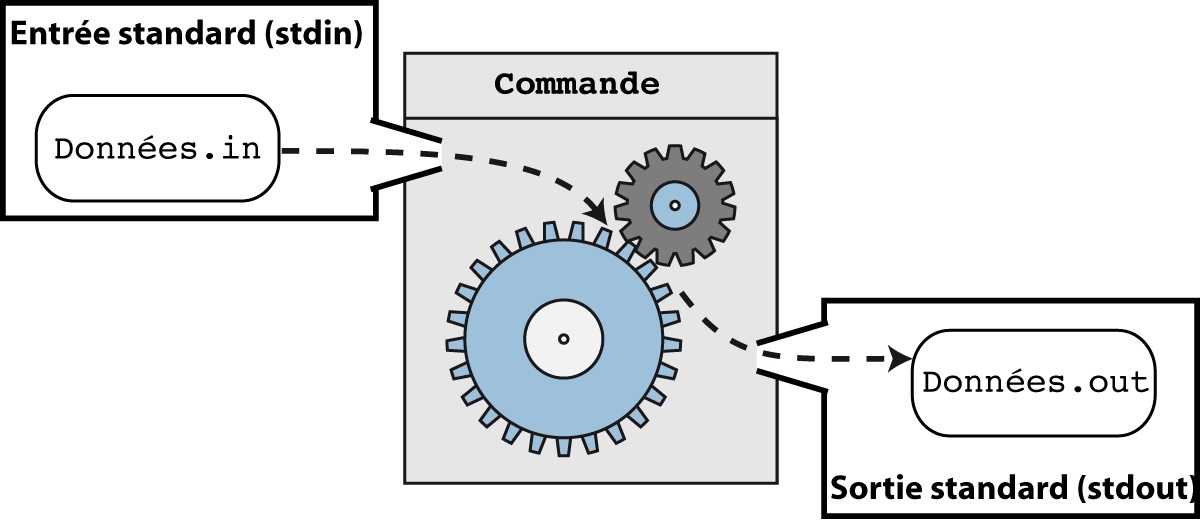
\includegraphics[width=6cm]{img/s05/stdin_stdout_commande_1.jpg}
    \end{column}
  \end{columns}
  \begin{block}{Les flux de données}
    Pour fonctionner, un programme a donc besoin de lire des données
    (flux d'entrée: input) et d'écrire les résultats de ses évaluations
    (flux de sortie: output). On distingue 3 types de flux de données:
    \begin{itemize}
    \item \textbf{STDIN}: entrée standard (là où sont lues les données),
    \item \textbf{STDOUT}: sortie standard (là où sont écrits les
      résultats),
    \item \textbf{STDERR}: sortie erreur (là où sont écrit les messages
      d'erreur).
    \end{itemize}
  \end{block}
\end{frame}
\begin{frame}{Entrée et sortie standard}
  \begin{block}{Les commandes qui lisent sur l'entrée standard}
    \begin{itemize}
    \item Certaines commandes Linux qui traitent les données d'un
      fichier (dont le chemin est passé en paramètre) peuvent
      alternativement, si aucun chemin fichier n'est spécifié,
      travailler directement avec les données lues sur l'entrée
      standard.
    \item Par exemple: \lin{echo}, \lin{cat}, \lin{head}, \lin{tail},
      \lin{grep}.
    \item {\color{red}\textbf{Par défaut, l'entrée standard est le
          clavier}}.
    \end{itemize}
  \end{block}
  \begin{center}
    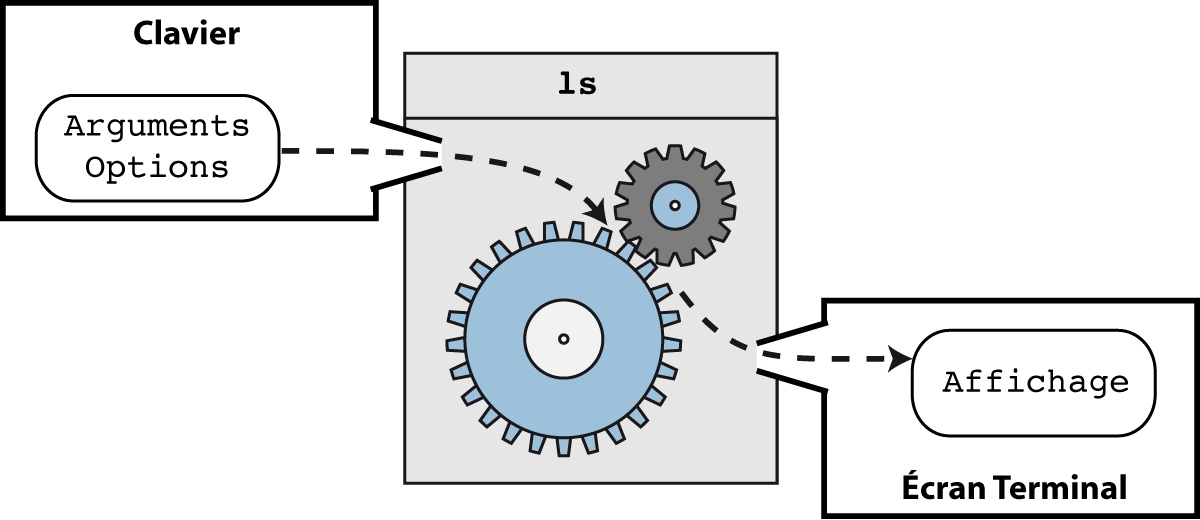
\includegraphics[width=6cm]{img/s05/stdin_stdout_commande_2.jpg}
  \end{center}
  \begin{block}{Les commandes qui écrivent sur la sortie standard}
    \begin{itemize}
    \item Les affichages produits par les commandes Linux sont le
      résultat de leur évaluation. Ce résultat est écrit sur la sortie
      standard.
    \item {\color{red}\textbf{Par défaut, la sortie standard est
          l'écran}}.
    \end{itemize}
  \end{block}
\end{frame}

%%%%%%%%%%%%%%% 

\manpage{cat}

\manpage{head}

\manpage{tail}

\manpage{grep}

\begin{exercice}
  \begin{exercicelet}{Manipulation du contenu d'un fichier texte}
    \begin{questions}
    \item La commande suivante montre le contenu d'un fichier texte:
      \begin{center}
        \small{ \mprompt{ \prompt[\~\//]{cat /proc/cpuinfo}{} } }
      \end{center}
    \item Quelle sont les informations contenues dans ce fichier?
    \item À l'aide des commandes \lin{cat} ou \lin{less} identifiez dans
      le fichier /proc/cpuinfo le nombre de fois ou le mot 'cpu'
      apparait
    \item La commande \lin{grep 'cpu' /proc/cpuinfo} permet d'afficher
      les lignes du fichier \lin{/proc/cpuinfo} où le mot 'cpu'
      apparait. Vérifiez qu'il y en le bon nombre?
    \item L'option -v permet d'inverser son comportement. Au lieu
      d'afficher les lignes qui présentent le motif, \lin{grep} affiche
      alors les lignes qui ne présentent pas le motif. Affichez les
      lignes du fichier \lin{/proc/cpuinfo} ne présentant pas le mot
      'cpu'.
    \item Proposez une commande permettant d'afficher les premières 5
      lignes
    \item Proposez une commande permettant d'afficher les dernières 5
      lignes
    \end{questions}
  \end{exercicelet}
\end{exercice}

%%%%%%%%%%%%%% 
\subsection{Redirections}
\begin{frame}{Redirection des Entrée/Sorties}
  \begin{block}{Commandes de Redirection}
    Il est possible de modifier le comportement par défaut des commandes
    et de donner une entrée et/ou une sortie standard différente des
    entrées/sorties standards.
    \begin{itemize}
    \item \mpromptS{\lin{command > fichier.out}}
      \begin{itemize}
      \item \textbf{{\color{solarizedRed}Redirige la sortie standard}} de la
        commande \lin{command} vers le fichier \lin{fichier.out}.
      \item Si le fichier \lin{fichier.out} n'existe pas, il est créé
        avec comme contenu les affichages produits par la commande
        \lin{command}.
      \item \textbf{{\color{solarizedBlue}Si le fichier \lin{fichier.out}
            existe, son contenu est écrasé}} et remplacé par les
        affichages produits par la commande \lin{command}.
      \end{itemize}
    \item \mpromptS{\lin{command >> fichier.out}}
      \begin{itemize}
      \item \textbf{{\color{solarizedRed}Redirige la sortie standard}} de la
        commande \lin{command} vers le fichier \lin{fichier.out}.
      \item Si le fichier \lin{fichier.out} n'existe pas, il est créé
        avec comme contenu les affichages produits par la commande
        \lin{command}.
      \item Si le fichier \lin{fichier.out} existe, les affichages
        produits par la commande \lin{command} sont
        \textbf{{\color{solarizedBlue}ajoutés à la fin du contenu du
            fichier}}.
      \end{itemize}
    \item \mpromptS{\lin{command 2> fichier.err}}
      \begin{itemize}
      \item \textbf{{\color{solarizedRed}Redirige la sortie erreur}} de la
        commande \lin{command} vers le fichier \lin{fichier.err}
        \textbf{{\color{solarizedBlue}avec écrasement du contenu}} si le
        fichier de sortie existe déjà.
      \end{itemize}
    \item \mpromptS{\lin{command 2>> fichier.err}}
      \begin{itemize}
      \item \textbf{{\color{solarizedRed}Redirige la sortie erreur}} de la
        commande \lin{command} vers le fichier \lin{fichier.err}
        \textbf{{\color{solarizedBlue}avec préservation du contenu}} si le
        fichier de sortie existe déjà.
      \end{itemize}
    \end{itemize}
  \end{block}
\end{frame}
%%%%%%%%%%%%%% 
\begin{frame}{Exemple de redirection}
  \begin{columns}
    \begin{column}{5.5cm}
      \begin{block}{Comportement par défaut de la commande \lin{ls}}
      \end{block}
      \begin{center}
        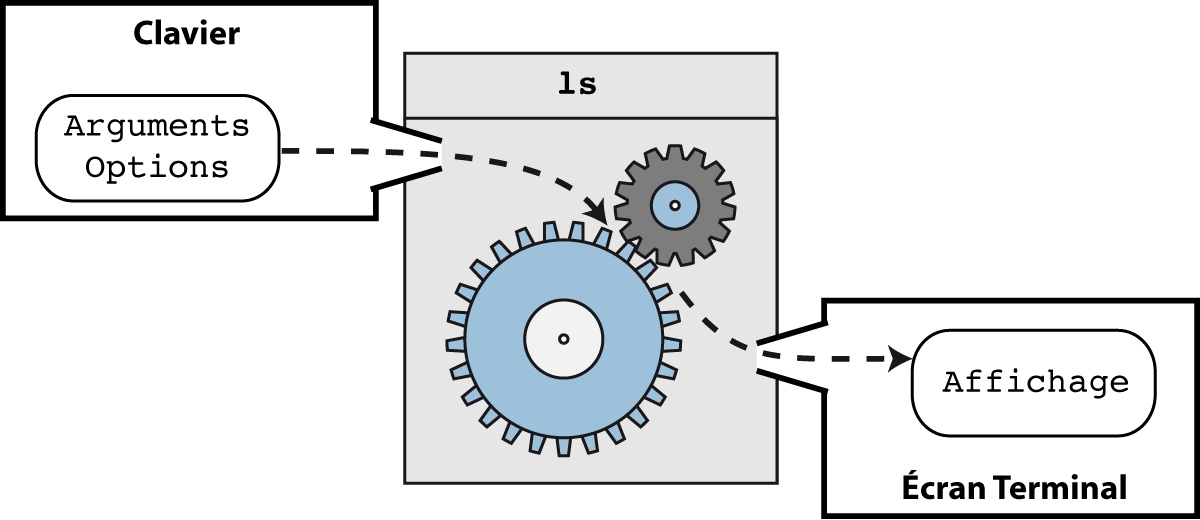
\includegraphics[width=5cm]{img/s05/stdin_stdout_commande_2.jpg}
      \end{center}
      \scriptsize{ \mpromptS{%
          \promptS{ls}{aldenaran.jpg alphacentauri.gif etacentauri.jpg}
          \promptS{ls}{aldenaran.jpg alphacentauri.gif etacentauri.jpg}
          \promptS{\cursor}{} } } La sortie standard de la première
      commande \lin{ls} est l'écran. La liste du contenu du répertoire
      courant est affichée à l'écran.\\\vspace{20pt}
    \end{column}
    \begin{column}{5.5cm}
      \begin{alertblock}{Redirection de la sortie de la commande
          \lin{ls}}
      \end{alertblock}
      \begin{center}
        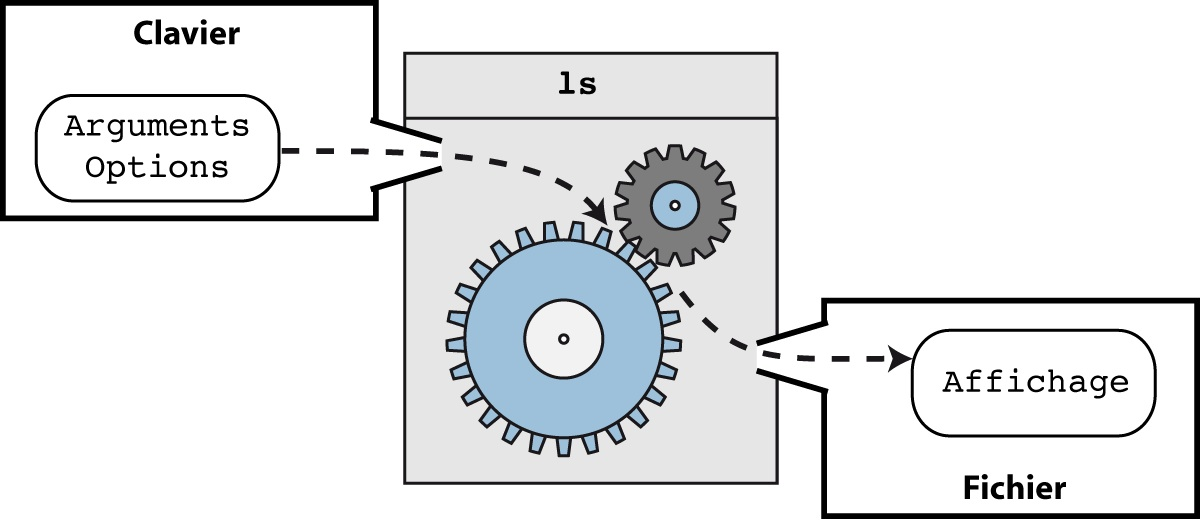
\includegraphics[width=5cm]{img/s05/stdin_stdout_commande_3.jpg}
      \end{center}
      \scriptsize{ \mpromptS{%
          \promptS{ls > {\color{solarizedBlue}1.out}}{}
          \promptS{ls}{{\color{solarizedBlue}1.out} aldenaran.jpg
            alphacentauri.gif etacentauri.jpg} \promptS{\cursor}{} } }
      La sortie standard de la première commande \lin{ls} est redirigée vers le fichier \lin{{\color{solarizedBlue}1.out}}. La liste du contenu du répertoire courant est écrite dans le fichier \lin{{\color{solarizedBlue}1.out}}.\\
      La deuxième commande \lin{ls}, montre qu'un fichier portant le nom
      \lin{{\color{solarizedBlue}1.out}} a été créé.\\\vspace{2pt}
    \end{column}
  \end{columns}
\end{frame}

%%%%%%%%%%%%%%%%%%%%%%%% 

\manpage{echo}

%%%%%%%%%%%%%%%%%%%%%%%% 

\begin{exercice}
  \begin{exercicelet}{Redirections}
    \begin{questions}
    \item Que font les commandes suivantes?
      % \begin{center}
      \small{ \mprompt{ \prompt{echo ``Bonjour"}{} \prompt{echo
            ``Bonjour" > bonjour.out}{} \prompt{echo ``Salut" >
            bonjour.out}{} \prompt{echo ``Bonjour" >> bonjour.out}{} }}
      % \end{center}
    \item Entrainez-vous avec les commandes suivantes. Profitez-en pour
      comprendre les affichages produits par les commandes \lin{ps} et
      \lin{file}:
      \begin{center}
        \mprompt{ \prompt{ps > essai\_ps.out}{} \prompt{file
            /usr/include/stdio.h > file.out}{} }
      \end{center}
    \item Proposez une commande pour copier le contenu de /proc/cpuinfo
      dans un fichier cpuinfo.out sans utiliser la commande \lin{cp}
    \end{questions}
  \end{exercicelet}
\end{exercice}

%%%%%%%%%%%%%% 
\subsection{Tubes}
\begin{frame}{Tubes}
  \begin{block}{Principes de fonctionnement des Tubes (Pipe en anglais)}
    \begin{itemize}
    \item A la différence des redirections simples qui permettent de
      rediriger la sortie standard d'une commande vers un fichier,
    \item {\color{solarizedRed}Un tube permet de rediriger la sortie standard
        d'une commande vers l'entrée standard d'une autre commande}.
    \end{itemize}
  \end{block}
  \begin{center}
    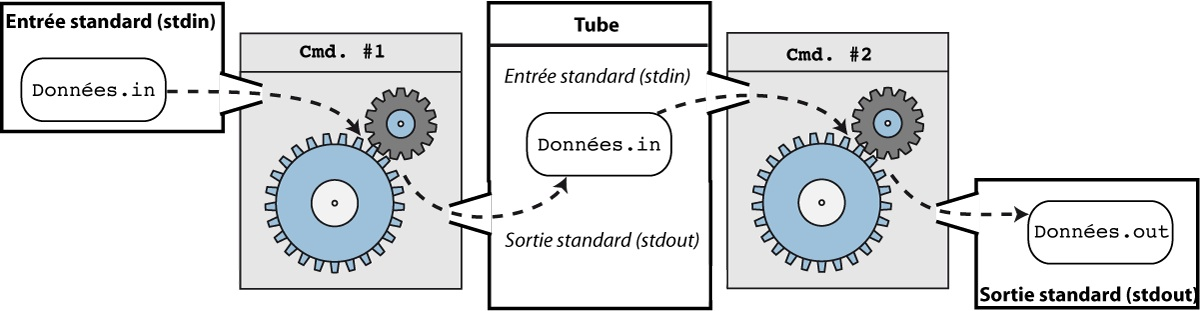
\includegraphics[height=2cm]{img/s05/stdin_stdout_tube_1.jpg}
  \end{center}
  \begin{alertblock}{Syntaxe}
    \begin{itemize}
    \item Le tube est symbolisé par le caractère \lin{|}.
    \item \mpromptS{ \lin{cmd1 | cmd2}}
      \begin{itemize}
      \item La sortie standard de la première commande (\lin{cmd1}) est
        redirigée vers l'entrée standard de la deuxième commande
        (\lin{cmd2}).
      \item L'entrée standard de la commande \lin{cmd1} et la sortie
        standard de la commande \lin{cmd2} ne sont pas modifiées.
      \end{itemize}
    \end{itemize}
  \end{alertblock}
\end{frame}


%%%%%%%%%%%%%% 
\begin{frame}{Exemple de Tubes avec les commande \lin{ls} et \lin{more}}
  \begin{block}{Rappel des commandes:}
    \begin{itemize}
    \item \lin{ls} affiche à l'écran (stdout) la liste des fichiers
      contenus dans un répertoire.
    \item \lin{more} affiche page par page le contenu des données passée
      sur son entrée standard.
    \end{itemize}
  \end{block}
  \begin{alertblock}{Exemple \#1}
    \begin{itemize}
    \item Si de très nombreux fichiers sont contenus dans un répertoire,
      la commande \lin{ls} peut produire un affichage qui ne tient pas
      dans l'écran, rendant impossible le parcours de la liste des
      fichiers (seuls les derniers sont visibles).
    \end{itemize}
    \begin{columns}
      \begin{column}{6cm}
        \small{ \mpromptS{%
            \promptS{ls}{} }\\\vspace{5pt} Défilement de tous les
          fichiers\\\vspace{5pt} \mpromptS{%
            \lin{%aldebaran.jpg alphacentauri.gif\\
              betelgeuse.jpg\hspace{2em}etacentauri.jpg\\soleil.jpg\hspace{4em}syrius.gif\\vega.png}\\
            \promptS{\cursor}{} } }
      \end{column}
      \begin{column}{6cm}
        \dirtree{%
          .1 \DTd{Images}\DTcomment{{\color{solarizedRed}Répertoire courant}}.
          .2 aldebaran.jpg\DTcomment{Hors de la fenetre}.  .2
          alphacentauri.gif\DTcomment{Hors de la fenetre}.  .2
          {\color{solarizedGreen}betelgeuse.jpg}\DTcomment{{\color{solarizedGreen}Dans
              la fenetre}}.  .2 {\color{solarizedGreen}
            etacentauri.jpg}\DTcomment{{\color{solarizedGreen}Dans la
              fenetre}}.  .2 {\color{solarizedGreen}
            soleil.jpg}\DTcomment{{\color{solarizedGreen}Dans la fenetre}}.
          .2 {\color{solarizedGreen}
            syrius.gif}\DTcomment{{\color{solarizedGreen}Dans la fenetre}}.
          .2 {\color{solarizedGreen}
            vega.png}\DTcomment{{\color{solarizedGreen}Dans la fenetre}}.
        }
      \end{column}
    \end{columns}
  \end{alertblock}
\end{frame}


%%%%%%%%%%%%%% 
\begin{frame}{Exemple de Tubes avec les commande \lin{ls} et \lin{more}}
  \begin{alertblock}{Exemple \#1 (suite):}
    \begin{itemize}
    \item La redirection de la sortie standard de la commande \lin{ls}
      vers l'entrée standard de la commande \lin{more} permet de passer
      en revue l'affichage de la commande \lin{ls} page par page.
    \end{itemize}
    \begin{center}
      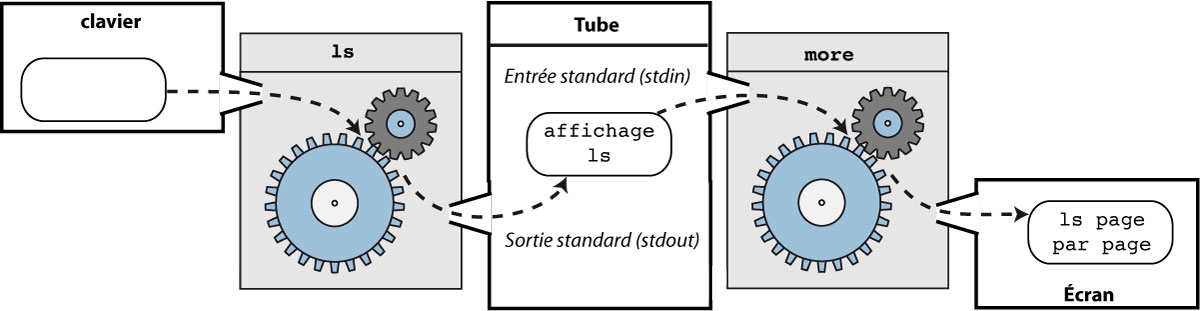
\includegraphics[height=2cm]{img/s05/stdin_stdout_tube_ls_more.jpg}
    \end{center}
    \begin{columns}
      \begin{column}{6cm}
        \small{ \mpromptS{%
            \promptS{ls | more}{aldebaran.jpg\hspace{2.5em}alphacentauri.gif\\
              betelgeuse.jpg\hspace{2em}etacentauri.jpg\\soleil.jpg\hspace{4em}syrius.gif}
          }\\
          Affichage d'une première page puis \\
          Presser la touche \Enter pour la page suivante\\
          \mpromptS{%
            \lin{soleil.jpg\hspace{4em}syrius.gif\\vega.png}\\
            \promptS{\cursor}{} } }
      \end{column}
      \begin{column}{6cm}
        \dirtree{%
          .1 \DTd{Images}\DTcomment{{\color{solarizedRed}Répertoire courant}}.
          .2 aldebaran.jpg\DTcomment{Page 1}.  .2
          alphacentauri.gif\DTcomment{Page 1}.  .2
          betelgeuse.jpg\DTcomment{Page 1}.  .2
          etacentauri.jpg\DTcomment{Page 1}.  .2
          soleil.jpg\DTcomment{Page 1\&2}.  .2 syrius.gif\DTcomment{Page
            1\&2}.  .2 vega.png\DTcomment{Page 2}.  }
      \end{column}
    \end{columns}
  \end{alertblock}
\end{frame}

%%%%%%%%%%%%%% 
\begin{frame}{Exemple de Tubes avec les commande \lin{ls} et \lin{grep}}
  \begin{block}{Rappel des commandes:}
    \begin{itemize}
    \item \lin{ls} affiche à l'écran (stdout) la liste des fichiers
      contenus dans un répertoire.
    \item \lin{grep} affiche les lignes d'un texte qui comportent un
      certain motif.
    \end{itemize}
  \end{block}
  \begin{alertblock}{Exemple \#2:}
    \begin{itemize}
    \item Si de très nombreux fichiers sont contenus dans un répertoire,
      la commande \lin{ls} peut produire un affichage qui ne tient pas
      dans l'écran, rendant compliqué l'identification de certain type
      de fichier (fichiers au format \lin{gif} par exemple).
    \end{itemize}
    \begin{columns}
      \begin{column}{6cm}
        \small{ \mpromptS{%
            \promptS{ls}{aldebaran.jpg\\alphacentauri.gif\\betelgeuse.jpg\\etacentauri.jpg\\soleil.jpg\\syrius.gif\\vega.png}
            \promptS{\cursor}{} } }
      \end{column}
      \begin{column}{6cm}
        \dirtree{%
          .1 \DTd{Images}\DTcomment{{\color{solarizedRed}Répertoire courant}}.
          .2 aldebaran.jpg\DTcomment{Affiché}.  .2
          alphacentauri.gif\DTcomment{Affiché}.  .2
          betelgeuse.jpg\DTcomment{Affiché}.  .2
          etacentauri.jpg\DTcomment{Affiché}.  .2
          soleil.jpg\DTcomment{Affiché}.  .2
          syrius.gif\DTcomment{Affiché}.  .2
          vega.png\DTcomment{Affiché}.  }
      \end{column}
    \end{columns}
  \end{alertblock}
\end{frame}

%%%%%%%%%%%%%% 
\begin{frame}{Exemple de Tubes avec les commande \lin{ls} et \lin{more}}
  \begin{alertblock}{Exemple \#2 (suite):}
    \begin{itemize}
    \item La redirection de la sortie standard de la commande \lin{ls}
      vers l'entrée standard de la commande \lin{grep} permet
      d'effectuer un filtrage des fichiers présents dans le répertoire
      sur la base d'un motif présent dans leur nom (par exemple
      l'extension \lin{.gif}).
    \end{itemize}
    \begin{center}
      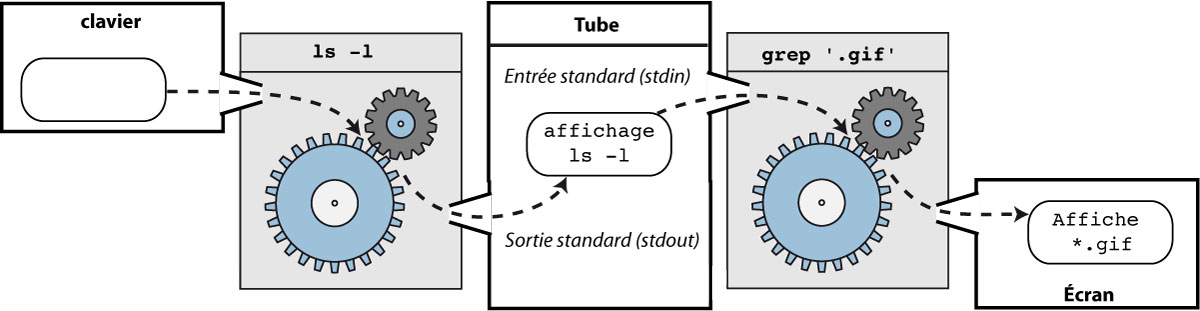
\includegraphics[height=2cm]{img/s05/stdin_stdout_tube_ls_grep.jpg}
    \end{center}
    \begin{columns}
      \begin{column}{6cm}
        \small{ \mpromptS{%
            \promptS{ls | grep '.gif'}{alphacentauri.gif\\syrius.gif}
            \promptS{\cursor}{} } }
      \end{column}
      \begin{column}{6cm}
        \dirtree{%
          .1 \DTd{Images}\DTcomment{{\color{solarizedRed}Répertoire courant}}.
          .2 aldebaran.jpg\DTcomment{Retenu par le filtre}.  .2
          alphacentauri.gif\DTcomment{Affiché}.  .2
          betelgeuse.jpg\DTcomment{Retenu par le filtre}.  .2
          etacentauri.jpg\DTcomment{Retenu par le filtre}.  .2
          soleil.jpg\DTcomment{Retenu par le filtre}.  .2
          syrius.gif\DTcomment{Affiché}.  .2 vega.png\DTcomment{Retenu
            par le filtre}.  }
      \end{column}
    \end{columns}
  \end{alertblock}
\end{frame}

%%%%%%%%%%%%%% 

\manpage{wc}

%%%%%%%%%%%% 

\begin{exercice}
  \begin{exercicelet}{Tubes}
    \begin{questions}
    \item Étudiez et comparez les commandes suivantes. Pour vous aider
      vous pouvez évaluer les commandes pas à pas en vous arrêtant avant
      chaque tube.
      % \begin{center}
      \small{ \mprompt{ \prompt{cat /proc/cpuinfo | wc -l}{}
          \prompt{head /proc/cpuinfo | wc -l}{} \prompt{cat
            /proc/cpuinfo | grep 'cpu' | wc -l}{} \prompt{head
            /proc/cpuinfo | grep 'cpu' | wc -l}{} }}
      % \end{center}
    \item Proposez une commande pour afficher le nombre de fichiers dans
      votre répertoire home
    \item Proposez une commande pour afficher le nombre des processus
    \item Proposez une commande pour afficher les premières 5 lignes des
      dernières 10 lignes du fichier /proc/cpuinfo
    \end{questions}
  \end{exercicelet}
\end{exercice}


\section{Les scripts Bash}
\subsection{Introduction}
\begin{frame}{Rappel}
  \begin{block}{Les interpréteurs}
    \begin{itemize}
    \item L'interpréteur parcourt le texte tapé par l'utilisateur, identifie les commandes et les paramètres, et si la syntaxe est correcte, lance un processus.
    \item Plusieurs interpréteurs existent : csh, tcsh, bash.
    \item Bash est l’interpréteur du projet GNU. Il est le plus utilisé sous linux. C'est Bash l'interpréteur qu'on utilise dans ce cours.
    \item L'interpréteur peut lire les commandes à partir d'un fichier, le \emph{script} shell.
    \end{itemize}
  \end{block}
\end{frame}

\begin{frame}[fragile]{Introduction}
  \begin{block}{Structure d'un script Bash}
    \begin{itemize}
    \item Un script Bash commence toujours par la ligne \alert{\#!/bin/bash} , suivi par une série d'instructions et commentaires (optionels)
    \item Un commentaire est une partie rédigée du script qui ne sera pas considérée comme une instruction lors de l'exécution du script. Pour commenter une portion du script on utilise le caractère \#. L'ensemble du texte situé sur la même ligne et après le carcactère \# sera considéré comme un commentaire et ne sera pas évalué.
    \end{itemize}
  \end{block}

  \begin{block}{Exemple}
    \begin{center}
\begin{verbatim}
#!/bin/bash
echo Liste des Fichiers:
#affiche la liste
ls
\end{verbatim}
    \end{center}
  \end{block}
\end{frame}

\begin{frame}[fragile]{Introduction}
  \begin{block}{Execution d'un script}
    \begin{itemize}
    \item Un script est un simple fichier texte (habituellement, ils ont l'extension \alert{.sh}) . Pour l'executer, il faut avant tout le rendre exécutable: \verb|chmod u+x script.sh|
    \item Maintenant, on peut l'exécuter en faisant: \verb|./script.sh|
    \item On peut aussi le lancer en appelant explicitement l'interpréteur: \verb|bash script.sh|
    \end{itemize}
  \end{block}


  \begin{exercicelet}{Premier script Bash}
    \begin{questions}
    \item Après avoir créé un repertoire nommé \texttt{~/Intro\_Systeme/TP\_3/scripts/}, écrivez et exécutez un script \texttt{exo\_0\_script.sh} qui affiche à l'écran le nombre de fichiers contenus dans le repertoire courant, après un message de texte "Nombre de fichiers:"
    \end{questions}
  \end{exercicelet}


\end{frame}


\begin{exercice}
  \begin{exercicelet}{Introduction aux scripts Bash}
    \begin{questions}
    \item Définissez et exécutez un script nommé \texttt{exo\_1\_script.sh} qui réalise la suite de commandes suivante: \texttt{echo "Debut"; sleep 2; echo "Apres 2 sec."; sleep 5; echo "Apres 5sec"}
    \item Que se passe-t-il si vous commentez les lignes commencant par la commande sleep?
    \item Définissez un script \texttt{exo\_2\_script.sh} qui affiche "Bonjour", définit le répertoire \texttt{~/Intro\_Systeme/TP\_3/scripts/} comme répertoire courant, puis crée dans celui-ci un répertoire \texttt{Test}, et finalement copie dans \texttt{Test} le fichier \texttt{/proc/cpuinfo}.
    \item Définissez un script nommé \texttt{exo\_3\_script.sh} qui affiche le contenu du répertoire \texttt{Test}, puis supprime le fichier \texttt{cpuinfo} y contenu (\texttt{Test/cpuinfo}), et finalement crée dans \texttt{Test} un fichier \texttt{infoCPU.txt} composé par les lignes du fichier \texttt{/proc/cpuinfo} qui contiennent le mot \texttt{'cpu'}.
    \end{questions}
  \end{exercicelet}
\end{exercice}

\subsection{Variables et Paramètres}
\begin{frame}[fragile]{Les Variables}
  \begin{block}{Les variables en Bash}
    \begin{itemize}
    \item Pour affecter une valeur à une variable c'est très simple. Il suffit d'écrire \texttt{nom\_variable=valeur}
    \item Pour accéder au contenu d'une variable, il faut utiliser le préfixe \lin{\$}
      % \item Pour supprimer une variable, il faut utiliser l'instruction \lin{unset}.
    \item On peut accéder aussi aux variables d'environnement, qui ont été définies ailleurs (par exemple \texttt{\$PATH}) 
    \end{itemize}
  \end{block}

  \begin{block}{Exemple}
\begin{verbatim}
MSG=Bonjour
echo $MSG
echo $PATH
\end{verbatim}
  \end{block}

  \begin{exercicelet}{Les Variables}
    \begin{questions}
    \item Définissez un script nommé \texttt{exo\_4\_script.sh} à partir du script \texttt{exo\_2\_script.sh}, et modifiez-le pour que le nom du répertoire \texttt{Test/} soit une variable dans le script.
    \end{questions}
  \end{exercicelet}
  
\end{frame}

\begin{frame}[fragile]{Les Paramètres}
  \begin{block}{Les paramètres}
    \begin{itemize}
    \item Il s'agit d'unes variables spéciales qui contiennent les arguments fournis au script par la ligne de commandes
    \item \textbf{\$0}: nom du script
    \item \textbf{\$1 \$2 ... }: paramètres en position 1, 2, ...
    \item \textbf{\$\#}: nombre de paramètres positionnels
    \item \textbf{\$*}: ensemble des paramètres
    \end{itemize}
  \end{block}

  \begin{block}{Exemple}
    \small{
      Soit \texttt{arg.sh} le script suivant:
\begin{verbatim}
#!/bin/bash
echo "Nombre d'argument "$#
echo "Les arguments sont "$*
echo "Le second argument est "$2
\end{verbatim}
      \vspace{0.1cm}
      \promptM{./arg.sh A B C}{
	Nombre d'argument 3 \\
	Les arguments sont A B C \\
	Le second argument est B
      }
    }
  \end{block}
  
\end{frame}

\begin{exercice}
  \begin{exercicelet}{Introduction aux scripts Bash}
    \begin{questions}
    \item Définissez un script nommé \texttt{exo\_5\_script.sh} à partir du script \texttt{exo\_2\_script.sh}, et modifiez-le pour que le nom du répertoire \texttt{Test/} soit passé comme un paramètre du script.
    \item Rédigez un script recevant 3 paramètres (nom, prénom et serveur) permettant l'affichage d'une adresse mail formatée (nom.prénom@serveur)

    \end{questions}
  \end{exercicelet}
\end{exercice}

\section{Structures de contrôle en BASH}
\subsection{Les calculs arithmétiques}
\begin{frame}{Les calculs arithmétiques}
  \begin{alertblock}{\lin{Bash} un langage orienté sur le traitement des chaînes de caractères}
    Même si ce langage n'est pas fait pour effectuer des opérations de calcul arithmétique il propose des fonctionnalités de base permettant d'effectuer des calculs simples tels que les additions, soustractions, multiplications et divisions. 
  \end{alertblock}
  \begin{block}{Syntaxe}
    \begin{center}
      \linbox{\$(( \it{expression\_arithmétique} ))}
    \end{center}
  \end{block}
  \begin{block}{Exemples}
    \begin{center}
      \tiny{%
        \mpromptS{%
          \promptS{total=\$(( 5 + 3 ))}{}
          \promptS{echo \$total}{8}
          \promptS{echo \$(( 5 - 3 ))}{2}
          \promptS{echo \$(( 5 * 3 ))}{15}
          \promptS{echo \$(( 5 / 3 ))}{1}
        }
      }
    \end{center}
  \end{block}
\end{frame}

\begin{exercice}
  \begin{exercicelet}{Les calculs arithmétiques}
    \begin{questions}
    \item Proposez une suite de 2 commandes affectant à une variable \texttt{res} le résultat des opérations arithmétiques suivantes et affichant le résultat contenu dans cette variable: $5 + 7$ et $3 * 2$
    \item Proposez une suite de 3 commandes permettant:
      \begin{itemize}
      \item d'affecter à une variable \texttt{res} la valeur $3$,
      \item d'ajouter $13$ à la variable \texttt{res},
      \item d'afficher le résultat de l'addition stockée dans la variable \texttt{res}.
      \end{itemize}


    \end{questions}
  \end{exercicelet}
\end{exercice}

\subsection{La boucle for}
\begin{frame}{\lin{for}}
  \begin{columns}
    \begin{column}{5cm}
      \begin{block}{\lin{for} Boucle itérative}
        \begin{itemize}
        \item permet de répéter l'évaluation d'une ou plusieurs instructions,
        \item à chaque tour de boucle une variable appelée itérateur change de valeur,
        \item la sortie de boucle s'effectue lorsque l'itérateur atteint une certaine valeurs.
        \end{itemize}
      \end{block}
    \end{column}
    \begin{column}{6cm}
      \begin{block}{Syntaxe \#1}
        \begin{center}
          \mpromptS{%
            for ((\it{ init ; test ; incr })); do\\
            \hspace*{2em}expr\_1\\
            \hspace*{2em}expr\_2\\
            \hspace*{2em}\dots\\
            done
          }
        \end{center}
        Ici, la condition d'arrêt est sur la valeur numérique de l'itérateur.
      \end{block}
    \end{column}
  \end{columns}
  \begin{block}{Exemple \#1}
    \small{%
      \begin{columns}
        \begin{column}{5cm}
          \fileform[5cm]{test\_for\_loop\_1.bash}{\#!/bin/bash\\\\echo "test \#1"\\for (( i = 0 ; i < 3 ; i++ ));do\\\hspace*{2em}echo '\$i = '\$i\\done}
        \end{column}
        \begin{column}{5.5cm}
          \mpromptS{%
            \promptS{./test\_for\_loop\_1.bash}{test \#1\\\$i = 0\\\$i = 1\\\$i = 2}
          }
        \end{column}
      \end{columns}
    }
  \end{block}
\end{frame}
%%%%%%%%%%%%%% 
\begin{frame}{\lin{for}}
  \begin{columns}
    \begin{column}{5cm}
      \begin{block}{\lin{for} Boucle itérative}
        \begin{itemize}
        \item permet de répéter l'évaluation d'une instruction,
        \item à chaque tour de boucle une variable appelée itérateur change de valeur,
        \item la sortie de boucle s'effectue lorsque l'itérateur a parcouru toute la liste.
        \end{itemize}
      \end{block}
    \end{column}
    \begin{column}{6cm}
      \begin{block}{Syntaxe \#2}
        \begin{center}
          \mpromptS{%
            for var in val\_1 val\_2 \dots; do\\
            \hspace*{2em}expr\_1\\
            \hspace*{2em}expr\_2\\
            \hspace*{2em}\dots\\
            done
          }
        \end{center}
        Ici, la boucle s'arrête lorsque toute la liste des valeurs a été parcourue.
      \end{block}
    \end{column}
  \end{columns}
  \begin{block}{Exemple \#2}
    \small{%
      \begin{columns}
        \begin{column}{5cm}
          \fileform[5cm]{test\_for\_loop\_2.bash}{\#!/bin/bash\\\\echo "test \#2"\\for i in hello la terre;do\\\hspace*{2em}echo '\$i = '\$i\\done}
        \end{column}
        \begin{column}{5.5cm}
          \mpromptS{%
            \promptS{./test\_for\_loop\_2.bash}{test \#2\\\$i = hello\\\$i = la\\\$i = terre}
          }
        \end{column}
      \end{columns}
    }
  \end{block}
\end{frame}

\begin{exercice}
  \begin{exercicelet}{La boucle \texttt{for}}
    \begin{questions}
    \item Dans le cours nous avons vu plusieurs syntaxes possibles pour la boucle for. Soit le script suivant:
      \begin{minipage}[c]{5cm}
\begin{verbatim}
#!/bin/bash
# affiche les 10 premiers entiers pairs
for int in 2 4 6 8 10 12 14 16 18 20
do
echo $int
done   
\end{verbatim}
      \end{minipage}

    \item Modifiez ce script pour remplacer la liste de valeurs par une expression arithmétique

    \end{questions}
  \end{exercicelet}
\end{exercice}

\subsection{Les branchements conditionnels if}
\begin{frame}{\lin{if}}
  \begin{block}{Branchements conditionnels}
    \begin{itemize}
    \item Le \lin{if} permet de mettre en place des alternatives.
    \item Un test (dont le résultat est Vrai ou Faux) permet de conditionner les expressions qui seront évaluées.
    \end{itemize}
  \end{block}\vrule
  \begin{columns}
    \begin{column}{6cm}
      \begin{block}{Syntaxe \#1}
        \mpromptS{%
          if test\\
          then\\
          \hspace*{2em}expr\_1\\
          \hspace*{2em}expr\_2\\
          \hspace*{2em}\dots\\
          fi
        }
      \end{block}
    \end{column}
    \begin{column}{5cm}
      \begin{block}{Comportement}
        \begin{itemize}
        \item Ici, les expressions ne sont évaluées que si le test renvoie la valeur Vrai.\\
        \item Aucune des expressions ne sont évaluées si le test renvoie la valeur Faux.
        \end{itemize}
      \end{block}
    \end{column}
  \end{columns}
\end{frame}
%%%%%%%%%%%%%% 
\begin{frame}{\lin{if}}
  \begin{columns}
    \begin{column}{6cm}
      \begin{block}{Syntaxe \#2}
        \mpromptS{%
          if test\\
          then\\
          \hspace*{2em}expr\_1\\
          else\\
          \hspace*{2em}expr\_2\\
          fi
        }
      \end{block}
    \end{column}
    \begin{column}{5cm}
      \begin{block}{Comportement}
        \begin{itemize}
        \item Si le test renvoie la valeur Vrai l'expression \lin{expr\_1} est évaluée, et\\
        \item sinon le test renvoie la valeur Faux c'est l'expression \lin{expr\_2} qui est évaluée.
        \end{itemize}
      \end{block}
    \end{column}
  \end{columns}
  \begin{columns}
    \begin{column}{6cm}
      \begin{block}{Syntaxe \#3}
        \mpromptS{%
          if test\_1\\
          then\\
          \hspace*{2em}expr\_1\\
          elif test\_2\\
          then\\
          \hspace*{2em}expr\_2\\
          elif test\_3\\
          then\\
          \hspace*{2em}expr\_3\\
          else\\
          \hspace*{2em}expr\_4\\
          fi
        }
      \end{block}
    \end{column}
    \begin{column}{5cm}
      \begin{block}{Comportement}
        \begin{itemize}
        \item Si \lin{test\_1} renvoie la valeur Vrai l'expression \lin{expr\_1} est évaluée,\\
        \item si \lin{test\_2} renvoie la valeur Vrai l'expression \lin{expr\_2} est évaluée,\\
        \item si \lin{test\_3} renvoie la valeur Vrai l'expression \lin{expr\_3} est évaluée, et\\
        \item si aucun des tests ne renvoie la valeur Vrai alors c'est l'expression \lin{expr\_4} qui est évaluée.
        \end{itemize}
      \end{block}
    \end{column}
  \end{columns}
\end{frame}
%%%%%%%%%%%%%% 
\begin{frame}{Les tests}
  \begin{block}{Les tests peuvent prendre plusieurs formes}
    Il peuvent porter sur:
    \begin{itemize}
    \item l'arborescence (présence, absence, permission sur les répertoires et fichiers),
    \item les chaînes de caractères,
    \item les valeurs numériques.
    \end{itemize}
  \end{block}
  \begin{block}{Tests de l'arborescence}
    \begin{center}
      \begin{tabular}{ll}
        \hline\\
        Syntaxe&Valeur\\
        \hline\\
        $[$ -d fichier$]$&Vrai si fichier est un nom de répertoire valide (si il existe).\\[3pt]
        $[$ -f fichier $]$&Vrai si fichier est un nom de fichier valide (si il existe).\\[3pt]
        $[$ -r fichier $]$&Vrai si il y a le droit de lecture sur le fichier.\\[3pt]
        $[$ -w fichier$]$&Vrai si il y a le droit d'écriture sur le fichier.\\[3pt]
        $[$ -x fichier $]$&Vrai si il y a le droit d'exécution sur le fichier.\\[3pt]
        \hline
      \end{tabular}
    \end{center}
  \end{block}
\end{frame}
%%%%%%%%%%%%%%%%%% 
\begin{exercice}
  \begin{exercicelet}{Tests de l'arborescence}
    \begin{questions}
    \item Créez un script \texttt{ico\_existe.sh}, qui teste si un fichier \texttt{ico} est présent dans le répertoire courant. Si le fichier existe, le script affiche le message d'avertissement suivant (\$PWD sera remplacé lors de l'exécution par la valeur de la variable d'environnement):
      \begin{minipage}[c]{5cm}
\begin{verbatim}
Attention: le fichier $PWD/ico existe
\end{verbatim}
      \end{minipage}
      
      
    \item Modifiez le script pour qu’il supprime le fichier \texttt{ico} si celui-ci existe et affiche un message d'avertissement indiquant que le fichier est supprimé. Les affichages seront alors les suivants:
      \begin{minipage}[c]{5cm}
\begin{verbatim}
Attention: le fichier $PWD/ico existe
Le Fichier $PWD/ico est supprime
\end{verbatim}
      \end{minipage}
    \item Modifiez ce script pour qu'il teste en plus si le répertoire courant contient un répertoire nommé \texttt{ico/}. Si il ne contient pas de répertoire \texttt{ico/}, le script crée ce répertoire.
    \end{questions}
  \end{exercicelet}
\end{exercice}

%%%%%%%%%%%%%% 
\begin{frame}{Les tests}
  \begin{block}{Tests sur les chaînes de caractères}
    \begin{center}
      \begin{tabular}{ll}
        \hline\\
        Syntaxe&Valeur\\
        \hline\\
        $[$ chaine\_1 = chaine\_2 $]$&Vrai si les 2 chaînes sont identiques.\\[2pt]
        $[$ chaine\_1 != chaine\_2 $]$&Vrai si les 2 chaînes sont différentes.\\[2pt]
        $[$ -n chaine $]$&Vrai si la chaîne est non vide.\\[2pt]
        $[$ -z chaine $]$&Vrai si la chaîne est vide.\\[2pt]
        \hline
      \end{tabular}
    \end{center}
  \end{block}
  
  \begin{exercicelet}{Tests sur les chaînes}
    \begin{questions}
    \item Définissez un script \texttt{testPWD.sh} qui prend en paramètre une chaîne de caractères et la compare avec la variable d'environnement \texttt{\$PWD}, il doit afficher 'OK' si le paramètre correspond à la valeur de la variable, 'Non' en cas contraire.
    \end{questions}
  \end{exercicelet}
  
\end{frame}

\begin{frame}{Les tests}
  \begin{block}{Tests sur les valeurs numériques}
    \begin{center}
      \begin{tabular}{ll}
        \hline\\
        Syntaxe&Valeur\\
        \hline\\
        $[$ nb\_1 -eq nb\_2 $]$&Vrai si nb\_1 = nb\_2 (eq pour equal).\\[2pt]
        $[$ nb\_1 -ne nb\_2 $]$&Vrai si nb\_1 $\neq$ nb\_2 (ne pour not equal).\\[2pt]
        $[$ nb\_1 -gt nb\_2 $]$&Vrai si nb\_1 $>$ nb\_2 (gt pour greater than).\\[2pt]
        $[$ nb\_1 -ge nb\_2 $]$&Vrai si nb\_1 $\geq$ nb\_2 (ge pour greater or equal).\\[2pt]
        $[$ nb\_1 -lt nb\_2 $]$&Vrai si nb\_1 $<$ nb\_2 (ge pour lower than).\\[2pt]
        $[$ nb\_1 -le nb\_2 $]$&Vrai si nb\_1 $\leq$ nb\_2 (ge pour lower or equal).\\[2pt]
        \hline
      \end{tabular}
    \end{center}
  \end{block}

\end{frame}
%%%%%%%%%%%%%% 
\begin{frame}{Les tests}
  \begin{block}{Opérateurs booléens}
    \begin{center}
      \begin{tabular}{ll}
        \hline
        Syntaxe&Valeur\\
        \hline\\
        ! $[$ test $]$&NOT: Vrai si le test renvoie Faux (négation).\\[2pt]
        $[$ test\_1 $]$ $|$ $|$ $[$ test\_2 $]$&OU logique.\\[2pt]
        $[$ test\_1 $]$ \&\& $[$ test\_2 $]$&ET logique.\\[2pt]
        \hline
      \end{tabular}
    \end{center}
  \end{block}
  \begin{block}{Tables de vérité}
    \begin{columns}
      \begin{column}{5.5cm}
        \begin{center}
          \begin{tabular}{|l|l|l|}
            \hline
            \textbf{ET (\&\&)}&\textbf{Vrai}&\textbf{Faux}\\
            \hline
            \textbf{Vrai}&Vrai&Faux\\
            \hline
            \textbf{Faux}&Faux&Faux\\
            \hline
          \end{tabular}
        \end{center}
      \end{column}
      \begin{column}{5.5cm}
        \begin{center}
          \begin{tabular}{|l|l|l|}
            \hline
            \textbf{OU ($|$ $|$)}&\textbf{Vrai}&\textbf{Faux}\\
            \hline
            \textbf{Vrai}&Vrai&Vrai\\
            \hline
            \textbf{Faux}&Vrai&Faux\\
            \hline
          \end{tabular}
        \end{center}
      \end{column}
    \end{columns}
    \begin{center}
      \begin{tabular}{|l|l|l|}
        \hline
        \textbf{NOT (!)}&\textbf{Vrai}&\textbf{Faux}\\
        \hline
        &Faux&Vra\\
        \hline
      \end{tabular}
    \end{center}
  \end{block}
\end{frame}

\begin{exercice}
  \begin{exercicelet}{Tests sur les valeurs numériques}
    \begin{questions}
    \item Définissez un script \texttt{testTemp.sh} qui prend en paramètre une valeur numérique et une lettre ('C' ou 'F'). Si la lettre choisie est 'C', le script doit afficher 'chaud' si le paramètre numérique est plus grand que $25$, 'froid' si est moins que $10$, 'normal' dans les autres cas. Si la lettre choisie est 'F', il affiche 'chaud' si le paramètre numérique est plus grand que $78$ et 'froid' si le paramètre numérique est inférieur à $50$, 'normal' dans les autres cas. Si la lettre n'est pas 'C' ou 'F', il affiche un message d'erreur. 
    \end{questions}
  \end{exercicelet}
\end{exercice}

\begin{frame}[fragile]{Substitution de commande}
  \begin{block}{Un moyen de composer les instructions}
    La syntaxe \verb|$(commande avec des arguments)| est remplacée à
    l'exécution par le résultat de l'exécution dans un sous-shell de la
    commande \texttt{commande avec des arguments}.

    Cette fonctionnalité très puissante permet d'utiliser des commandes
    pour les affecter dans des variables et ensuite s'en servir dans le
    script.
  
    C'est une substitution
  \end{block}
  \begin{block}{Exemple}
    \begin{center}
\begin{verbatim}
#!/bin/bash
TITLE="En ce jour du $(date -I)"
MOTS=$(grep cool /usr/share/dict/words)
for i in $MOTS; do
  echo "$TITLE, $i est un mot cool"
done
\end{verbatim} %$
    \end{center}
  \end{block}

\end{frame}
\begin{exercice}
  \begin{exercicelet}{Archiveur}
    Faites un script qui a les actions suivantes si on lui donne en argument un répertoire (par exemple \verb|~/M1101/TD6|):
    \begin{questions}
    \item S'arrête si la cible n'est pas un répertoire
    \item Définit une variable BACKUPDIR qui vaut le chemin du répertoire du dessus suivi du mot \texttt{sauvegarde} (ici \verb|~/M1101/sauvegarde|) en utilisant la commande \texttt{dirname}
    \item Crée le répertoire s'il n'existe pas
    \item Définir une variable faite avec la date du jour et le nom du répertoire (par exemple 2014-10-31-TD6) en utilisante les commandes \texttt{basename} et \texttt{date}.
    \item Crée une archive compressée du répertoire (ici en exécutant \verb|tar czf ~/M1101/sauvegarde/2014-10-31-TD6.tgz ~/M1101/TD6|)
    \end{questions}
    On pourra affiner en s'arrêtant si une archive existe déjà sous ce
    nom avant de la créer (ou proposer de l'effacer en utilisant la
    commande \texttt{read x} pour lire une variable depuis le terminal).
  \end{exercicelet}
\end{exercice}

\end{document}

% Local Variables:
% TeX-master: "sys"
% TeX-PDF-mode: t
% fill-column: 78
% coding: utf-8-unix
% mode-require-final-newline: t
% mode: latex
% mode: flyspell
% ispell-local-dictionary: "francais"
% End:
